% Unfortunately for the contents to contain  the "Parts" lines successfully, hyperref needs to be disabled.
\documentclass[nohyper,nobib,a4,16pt]{tufte-book} %nobib

% There are usefull references heres: https://github.com/lalider/tufte-latex-thesis/blob/master/main.pdf

%%%%%%%%%%%%%%%%%%%%%%%%%%%%%%%%%%%%%
%%%%%%%%%%%%%% BOOK DATA %%%%%%%%%%%%%%
%%%%%%%%%%%%%%%%%%%%%%%%%%%%%%%%%%%%%
\title[PhD Thesis: infectious disease dynamics modeling towards informed control decisions]{Modelling infectious disease dynamics\\towards informed\\public-health\\interventions:\\ applications on \\COVID-19 and Cholera}
\date{\today}
\author[Joseph Lemaitre]{Joseph \ Lemaitre}
\publisher{Under the supervision of Prof. Andrea Rinaldo and Dr. Damiano Pasetto.}

%%%%%%%%%%%%%%%%%%%%%%%%%%%%%%%%%%%%%
%%%%%%%%%%%%%% PACKAGES %%%%%%%%%%%%%%%
%%%%%%%%%%%%%%%%%%%%%%%%%%%%%%%%%%%%%
\usepackage[utf8]{inputenc}
 \usepackage{pdfpages} % Include pdfs directly
 \usepackage[ruled,vlined]{algorithm2e} % algorithms
 \usepackage{nameref} % named references 
 \usepackage{url}
 \usepackage{ebgaramond} % Font I use, let's go baroque
 \usepackage[cmintegrals,cmbraces]{newtxmath}
 \usepackage{ebgaramond-maths} %exist for math too
\usepackage{booktabs}  % For nicely typeset tabular material
\usepackage{tabularx}
\usepackage{units}
\usepackage{xargs} % several argument in functions (needed for cite)
\usepackage[toc,page]{appendix}
%\usepackage{emoji} % I'd love to have emojis, but it doesn't work
%\setemojifont{TwemojiMozilla}
  % Set up the spacing using fontspec features
%\renewcommand\allcapsspacing[1]{{\addfontfeature{LetterSpace=15}#1}}
% \renewcommand\smallcapsspacing[1]{{\addfontfeature{LetterSpace=10}#1}}
 

% math stuff:
%\usepackage{amssymb} % does not play well with garamond math
\usepackage{amsbsy}
\usepackage{makecell}
\usepackage{amsmath}
\usepackage{bm}

% For graphics / images
\usepackage{graphicx}
\setkeys{Gin}{width=\linewidth,totalheight=\textheight,keepaspectratio}

% https://tex.stackexchange.com/questions/5017/center-column-with-specifying-width-in-table-tabular-enviroment define x for centered p in tabularx
\usepackage{array}
\newcolumntype{x}[1]{>{\centering\arraybackslash\hspace{0pt}}p{#1}}


%  margin figure caption header should to be smaller to remove this weird size diperempty:
% adapted from https://tex.stackexchange.com/questions/319345/change-font-size-in-caption-for-selected-figures, should post it there
\usepackage{caption}
\newcommand{\margincaption}[2][1={}]{%
  \captionsetup{font=footnotesize}%
  \caption[#1]{#2}}
% The fancyvrb package lets us customize the formatting of verbatim
% environment, so a slightly smaller font is used.
\usepackage{fancyvrb}
\fvset{fontsize=\normalsize}

%%%%%%%%%%%%%%%%%%%%%%%%%%%%%%%%%%%%%
%%%%%%%%%%%%% FRONTMATTER %%%%%%%%%%%%
%%%%%%%%%%%%%%%%%%%%%%%%%%%%%%%%%%%%%
% section in table of content
\setcounter{tocdepth}{3}
% pdf bookmarks, that are open to level 2
\usepackage[open,openlevel=2]{bookmark} %open up to level 2 by default
% Numbered chapters 
\setcounter{secnumdepth}{0}
%No link in TOC, that breaks tuftebook
\makeatletter
\let\Hy@linktoc\Hy@linktoc@none
\makeatother

% Prints an epigraph and speaker in sans serif, all-caps type.
\newcommand{\openepigraph}[2]{%
  %\sffamily\fontsize{14}{16}\selectfont
  \begin{fullwidth}
  \sffamily\large
  \begin{doublespace}
  \noindent\allcaps{#1}\\% epigraph
  \noindent\allcaps{#2}% author
  \end{doublespace}
  \end{fullwidth}
}
% Inserts a blank page
\newcommand{\blankpage}{\newpage\hbox{}\thispagestyle{empty}\newpage}


%%%%%%%%%%%%%%%%%%%%%%%%%%%%%%%%%%%%%
%%%%%%%% BIBLIOGRAPHY & CITATION %%%%%%%%
%%%%%%%%%%%%%%%%%%%%%%%%%%%%%%%%%%%%%
\usepackage[backend=biber,doi=false,isbn=false,url=false,eprint=false,style=verbose,citestyle=authoryear,maxbibnames=999,maxcitenames=1,citetracker=true,pagetracker=true,uniquename=false]{biblatex}%,firstinits=true, before: authoryear-comp; unique name is false :)
\addbibresource{../ZoteroLibUpdated/ZoteroLibUpdated.bib}

% Remove the In: if there is no journal title. But if not in my defined shortcite, it means that the publication type is ill-defined (should be online, or something without journal)
% Thanks to https://tex.stackexchange.com/questions/502657/how-to-remove-in-from-bibliography-if-there-is-no-journal-information
\renewbibmacro*{in:}{%
  \iffieldundef{journaltitle}
    {}
    {\printtext{\bibstring{in}\intitlepunct}}}
% remove it altogher
%\renewbibmacro*{in:}{;}
% a fullcite command described by removing stuff
\DeclareCiteCommand{\fullcite}
  {\usebibmacro{prenote}}
  {\clearfield{month}\clearfield{day}\clearfield{pages}\clearfield{volume}\clearfield{number}\clearfield{issue}\clearfield{urlyear}\clearfield{urlmonth}\clearfield{url}\clearfield{pagetotal}%\clearfield{title}\clearfield{journaltitle}%
   \usedriver
     {\DeclareNameAlias{sortname}{default}}
     {\thefield{entrytype}}}
  {\multicitedelim}
  {\usebibmacro{postnote}}
  
    \DeclareCiteCommand{\fullcite}
  {\usebibmacro{prenote}}
  {%
     \printnames[family]{labelname}% \printnames[given-family]{labelname}
     \setunit{\addcomma\space}%
     \printfield{title}%
     \setunit{\addspace}%addedme
  \usebibmacro{in:}%addedme
  \setunit{\addspace}%addedme
     \printfield{journaltitle}%
     \setunit{\addspace}%
     \printtext[parens]{%
       \printfield{year}}}%printdate
  {\multicitedelim}
  {\usebibmacro{postnote}}
  
  % a fullcite command described by adding stuff
  % Thanks https://tex.stackexchange.com/questions/490049/towards-a-concise-fullcite-command (also:https://tex.stackexchange.com/questions/479590/change-journaltitle-to-italics-in-fullcite, https://tex.stackexchange.com/questions/339681/abbreviate-journal-title-in-fullcite-command)
  \DeclareCiteCommand{\fullciteshorta}
  {\usebibmacro{prenote}}
  {%
     \printnames[family]{labelname}% \printnames[given-family]{labelname}
     \setunit{\addcomma\space}%
  %
     \printfield{journaltitle}%
     \setunit{\addspace}%
     \printtext[parens]{%
       \printfield{year}}}%printdate
  {\multicitedelim}
  {\usebibmacro{postnote}}
  
  \newbibmacro{aycite}{%
  \defcounter{maxnames}{1}%
  \ifnameundef{labelname}
    {\printfield{labeltitle}%
     \setunit{\printdelim{nonameyeardelim}}}
    {\printnames[family]{labelname}%
     \setunit{\printdelim{nameyeardelim}}}
  \printtext[bibhyperref]{\printlabeldateextra}}
  
\DeclareCiteCommand{\fullciteshortb}
  {\usebibmacro{prenote}}%
  {\usebibmacro{citeindex}%
   \usebibmacro{aycite}}
  {\multicitedelim}
  {\usebibmacro{postnote}} 

  %[][-\value{listtotal}]
  % from me: Remove the visited on https://tex.stackexchange.com/questions/400384/how-to-disable-biblatex-showing-visited-on-on-the-references
%\AtEveryBibitem{
  %  \clearfield{urlyear}
    %\clearfield{urlmonth}
%}
% Only year
%\AtEveryBibitem{\clearfield{month}}
%\AtEveryBibitem{}
%\AtEveryCitekey{\clearfield{month}\clearfield{day}\clearfield{pages}\clearfield{volume}\clearfield{number}\clearfield{issue}\clearfield{urlyear}\clearfield{urlmonth}\clearfield{pagetotal}\clearfield{publication}} % Remove day only in fullcite

\renewcommandx{\cite}[3][1={0pt},2={}]{\sidenote[][#1]{\fullcite[#2]{#3}.}}
\newcommandx{\shortcite}[3][1={0pt},2={}]{\sidenote[][#1]{\fullciteshortb[#2]{#3}.}}

% from me: short citation in sideline: https://tex.stackexchange.com/questions/414716/options-for-styling-fullcite
% No space: https://tex.stackexchange.com/questions/25891/fullcite-without-indent-in-biblatex ---> DELETED

%% Define \longfullcite to include all authors (https://tex.stackexchange.com/questions/142148/typeset-one-citation-with-all-authors)
\makeatletter
\DeclareCiteCommand{\longfullcite}
  {\usebibmacro{prenote}}
  {\usedriver
     {\c@maxnames\blx@maxbibnames\relax
      \DeclareNameAlias{sortname}{default}}
     {\thefield{entrytype}}}
  {\multicitedelim}
  {\usebibmacro{postnote}}
\makeatother

% Maybe this, but seems overkill: https://tex.stackexchange.com/questions/71526/repeat-the-same-reference-in-footnote-on-different-pages/71566#71566

%%%%%%%%%%%%%%%%%%%%%%%%%%%%%%%%%%%%%
%%%%%%%%%%%%%% HEADINGS %%%%%%%%%%%%%%
%%%%%%%%%%%%%%%%%%%%%%%%%%%%%%%%%%%%%

% --> I want titles ittle in Small capitals
\usepackage{titlesec}
%\usepackage{titletoc}
% Display instead of hang makes it on two line: Chapter 1\\blabla
\makeatletter
\titleformat{\chapter}[display]{\huge\scshape}{\@chapapp~\thechapter}{1em}{}%[\vspace{2ex}\titlerule]
\titleformat{\section}{\Large\scshape}{\thesection}{1em}{}
\titleformat{\subsection}{\large\scshape}{\thesubsection}{1em}{}
\titleformat{\paragraph}[runin]{\scshape}{\theparagraph}{}{}
\makeatother

% Table of contents. works well but should not use tocloft with titlesec
\usepackage[titles]{tocloft}
\renewcommand\cftchapfont{\scshape}
\renewcommand\cftsecfont{\scshape}
\renewcommand\cftsubsecfont{\scshape}
\renewcommand{\cftdot}{} %if fot inside, will put dots

%part from Kevin Godby, 
\titlecontents{part}%
    [0pt]% distance from left margin
    {\addvspace{0.25\baselineskip}}% above (global formatting of entry)
    {\allcaps{Part~\thecontentslabel}\allcaps}% before w/ label (label = ``Part I'')
    {\allcaps{Part~\thecontentslabel}\allcaps}% before w/o label
    {}% filler and page (leaders and page num)
    [\vspace*{0.5\baselineskip}]% after


%%%%%%%%%%%%%%%%%%%%%%%%%%%%%%%%%%%%%
%%%%%%%%%%%%%%% FULLFIGURE %%%%%%%%%%%%%%
%%%%%%%%%%%%%%%%%%%%%%%%%%%%%%%%%%%%%
% as per https://tex.stackexchange.com/questions/57413/change-caption-in-tufte-class-full-page-figure and https://tex.stackexchange.com/questions/229308/combining-tufte-latex-and-threeparttable/229419#229419 I want normal caption for full page figure... To do this: (I could have also used the fixed pull request by 
\RequirePackage{etoolbox}
\makeatletter
\newif\if@tufte@margtab\@tufte@margtabfalse
\AtBeginEnvironment{margintable}{\@tufte@margtabtrue}
\AtEndEnvironment{margintable}{\@tufte@margtabfalse}
\newcommand{\classiccaptionstyle}{%
    \long\def\@caption##1[##2]##3{%
        \par
        \addcontentsline{\csname ext@##1\endcsname}{##1}%
        {\protect\numberline{\csname the##1\endcsname}{\ignorespaces ##2}}%
        \begingroup
        \@parboxrestore
        \if@minipage
        \@setminipage
        \fi
        \normalsize
        \@makecaption{\csname fnum@##1\endcsname}{\ignorespaces ##3}\par
        \endgroup}
    \long\def\@makecaption##1##2{%
        \vskip\abovecaptionskip
        \sbox\@tempboxa{\@tufte@caption@font##1: ##2}%
        \ifdim \wd\@tempboxa >\hsize
        \@tufte@caption@font\if@tufte@margtab\@tufte@caption@justification\fi##1: ##2\par
        \else
        \global \@minipagefalse
        \hb@xt@\hsize{\hfil\box\@tempboxa\hfil}%
        \fi
        \vskip\belowcaptionskip}
       \setcaptionfont{\normalfont} % To have the rigght captio.n size
    \let\caption\@tufte@orig@caption%
    \let\label\@tufte@orig@label}
\makeatother


\newenvironment{fwfigure}{%
    \begin{figure*}[h!]
        \classiccaptionstyle
  }{\end{figure*}}
  \newenvironment{fwtable}{%
    \begin{table*}[h!]
        \classiccaptionstyle
  }{\end{table*}}

%%%%%%%%%%%%%%%%%%%%%%%%%%%%%%%%%%%%%
%%%%%%%%%%%%%%%%% MISC %%%%%%%%%%%%%%%%
%%%%%%%%%%%%%%%%%%%%%%%%%%%%%%%%%%%%%
% Prints argument within hanging parentheses (i.e., parentheses that take
% up no horizontal space).  Useful in tabular environments.
\newcommand{\hangp}[1]{\makebox[0pt][r]{(}#1\makebox[0pt][l]{)}}
% Prints an asterisk that takes up no horizontal space.
% Useful in tabular environments.
\newcommand{\hangstar}{\makebox[0pt][l]{*}}
% Prints a trailing space in a smart way.
\usepackage{xspace}
\newcommand{\hairsp}{\hspace{1pt}}% hair space
\newcommand{\ie}{\textit{i.\hairsp{}e.}\xspace}
\newcommand{\eg}{\textit{e.\hairsp{}g.}\xspace}
\newcommand{\na}{\quad--}% used in tables for N/A cells

\newcommand{\eqname}[1]{\tag*{#1}} %tag equations by name
% boxes
\usepackage[most]{tcolorbox}
\newtcolorbox{mybox}[1]{
    tikznode boxed title,
    enhanced,
    breakable, 
    arc=0mm,
    interior style={white},
    attach boxed title to top center= {yshift=-\tcboxedtitleheight/2},
    fonttitle=\bfseries,
    colbacktitle=white,coltitle=black,
    boxed title style={size=normal,colframe=white,boxrule=0pt},
    title={#1}}
%longer pages
\usepackage{geometry}
 \geometry{
 a4paper,
textheight=690pt,
 }

%Hyperref likes to be loaded last
\usepackage{hyperref}
 % prevent hyperref from destroying my lettrines https://tex.stackexchange.com/questions/561651/eb-garamond-initials-and-hyperref-package
%\DeclareTextFontCommand{\textin}{\initials}
%\usepackage{lettrine}
%\setcounter{DefaultLines}{5}
%\renewcommand{\LettrineFontHook}{\initials}


%%%%%%%%%%%%%%%%%%%%%%%%%%%%%%%%%%%%%
%%%%%%%%%%%%%%%%% DOC %%%%%%%%%%%%%%%%
%%%%%%%%%%%%%%%%%%%%%%%%%%%%%%%%%%%%%
\begin{document}
%\frontmatter
%\blankpage
%\begin{fullwidth}
\maketitle
\blankpage
\end{fullwidth}
% r.7 dedication
%\cleardoublepage
%~\vfill
%\begin{doublespace}
%\noindent\fontsize{18}{22}\selectfont\itshape
%\nohyphenation
%Dedicated to those who appreciate \LaTeX{} 
%and the work of \mbox{Edward R.~Tufte} 
%and \mbox{Donald E.~Knuth}.
%\end{doublespace}
%\vfill
%\vfill
%\end{fullwidth}
% r.9 introduction
%\cleardoublepage
%\begin{fullwidth}

\newenvironment{dedication}
  {\clearpage           % w- want a new page
   \thispagestyle{empty}% no header and footer
   \vspace*{\stretch{2}}% some space at the top 
   %\itshape             % the text is in italics
  
\leftskip=10cm
\raggedright
\parindent=0pt
\begin{fullwidth}
  }
  {\par % end the paragraph
   \vspace{\stretch{3}} % space at bottom is three times that at the top
   \clearpage           % finish off the page
\end{fullwidth}  }
 \begin{dedication}\textit{
\hspace{8.5cm}Vedrò con mio diletto \\
\hspace{8.5cm}L'alma dell'alma mia, dell'alma mia  \\
\hspace{8.5cm}Il core del mio cor  \\
\hspace{8.5cm}Pien di contento, pien di contento  \\
\hspace{8.5cm}Vedrò con mio diletto \\
\hspace{8.5cm}L'alma dell'alma mia, dell'alma mia \\
\hspace{8.5cm}Il cor di questo cor \\
\hspace{8.5cm}Pien di contento, pien di contento \\
\hspace{8.5cm}E se dal caro oggetto \\
\hspace{8.5cm}Lungi convien che sia, convien che sia \\
\hspace{8.5cm}Sospirerò penando \\
\hspace{8.5cm}Ogni momento \\
\hspace{8.5cm}Vedrò con mio diletto \\
\hspace{8.5cm}L'alma dell'alma mia, dell'alma mia \\
\hspace{8.5cm}Il core del mio cor \\
\hspace{8.5cm}Pien di contento, pien di contento \\
\hspace{8.5cm}Vedrò con mio diletto \\
\hspace{8.5cm}L'alma dell'alma mia, dell'alma mia \\
\hspace{8.5cm}Il cor di questo cor \\
\hspace{8.5cm}Pien di contento, pien di contento \\
%\hspace{11cm}-- Anastasio
}
%\hspace{8.5cm} \textit{On vise le Porsche Panamera et dire aux proches que ça ira.} \\
%\hspace{14cm}-- \textsc{Maes}
\end{dedication}

%\cleardoublepage


%\end{fullwidth}

  %\chapter*{Acknowledgements} \addcontentsline{toc}{chapter}{Acknowledgements}\markboth{Acknowledgements}{}
 
% Starting a PhD focused on infectious disease modeling has been an rewarding journey. I wish to thanks Professor Andrea Rinaldo first for the opportunity of exploring a new subject, but , for showing me the importance of a personnal contribution.  
 
 %Damiano, many thanks for making me stay employed and sane, for making this enjoyable, for all the good time spend together, and for your critical eye. I own you this thesis.
 
 %Scientifically, this thesis has benefited enormously from discussion and work with Javier. I have learnt so much and I am grateful
 
 %Mario Jacques
 
 %Upon my arrival at the ECHO lab in 2017, I've been welcomed by wonderful people who have made this journey fun. Thanks Silvia for the best tea cookie , Giezi and Luca, because sports and meta-science talks are meant to be. Later, Mitra, Cristiano and Paolo.
 
 
 %For my abbreviated mobility to Baltimore, I'd Prof. Justin Lessler and for trusting me  ... Elizabeth, Hannah, Kyu, Shaun have been welcoming. Thanks to the \textsc{covid} Scenario pipeline team, especially to Joshua Kamiski. Yeah, some people still uses emacs.
 
 %I have been fortunate to participate to GTFCC, to IDDConf 2019 and to SISMID 2019, thanks for the infectious disease modeling and connected public health communities have been so welcoming, greatly explaining. I learned and still learn from many. Standing on the shoulder of giants, 
 
 %This thesis makes use of many datasets from precipitation to reported cholera cases. I am very grateful to the workers all along the chain from collection to curation who have made my job possible.
 
 %Finally, thanks to reviewers, co-reviewers and co-authors from whom I have learned general concepts and valuable scientific writing tips.
 
%Tools shape the way you think about problems. This thesis was made possible, but also sculted by the languages and libraries I used. I want to acknowledge all the open-source maintainers and contributors who tirelessy make, document and maintain powerful tools, making the difficult easy and enabling everybody to use.

%À famille, papa, maman, pour m'avoir ouvert au monde et changer le regard sur les choses.

%À Céline, Eugène et Oliver, toujours près de mon coeur. %\emoji{smiling-face-with-hearts}\emoji{baby-light-skin-tone}

%Finallement, Marion ! Merci de m'avoir soutenue tout au long de cette incroyable voyage. Mais aussi d'avoir rendu cela serein et doux. 
 
 \chapter*{Summary} \addcontentsline{toc}{chapter}{Summary}\markboth{Summary}{}
 research problem and objectives

Public-health interventions strive to spare individuals and communities from the burden in infectious disease poses on humanity. Designing effective policies is an intricate task. Infectious disease epidemics are complex phenomena that results from the interaction between pathogens, individuals, environment and societies, and only scarce and biased information is available.  Modeling offers a principled way to deal with the available evidence to reason infectious disease dynamics, which in turn allow for informed control decisions.



compartmental models, diversity of models.

The present thesis tackles selected infectious disease modeling topics with the aim of helping decision-makers to design effective policies. 

%Your methods
A set of five modeling st of infectious disease transmission is proposed, each covering a different facet of the spread and control of disease.
Two mInitially focused on cholera, one of humanity's earliest disease, still present in many part of the world,  Model are used as representation of reality to 

The emergence of covid-19 in 2019 diverted the initial research plan focused on cholera, and we present modeling work , bridging the gap between science.


The final application of these model is within an optimal control framework, where algorithms designs the most effective SARS-CoV-2 vaccine allocation strategy




%Your key results
Results highlight 


%Your conclusion
This thesis Infectious disease modeling is a necessary, and the diversity 
 
\paragraph{Keywords} cholera, \textsc{covid}-19, infectious disease modeling,
epidemiology, optimal control, public health, inference
 
 
 \chapter*{Résumé} \addcontentsline{toc}{chapter}{Résumé}\markboth{Résumé}{}
 
 %\pdfbookmark[section]{\contentsname}{toc}
%\begin{fullwidth}\tableofcontents\listoffigures\listoftables\end{fullwidth}
%\pdfbookmark[section]{\contentsname}{toc}
%\begin{fullwidth}\tableofcontents\listoffigures\listoftables\end{fullwidth}

\mainmatter
% Modelling infectious disease dynamics towards informed public-health interventions, with application on \textsc{covid}-19 and cholera.
\chapter*{Introduction} % broad introductio
\addcontentsline{toc}{chapter}{Introduction}
\markboth{Introduction}{}
%epidemics as phenomena
 %d  unevenly distributed among populations. 
 % improverished communties around the world. %public health issue in many countries, and it's elimination of Global North countries -- . 
 \section{Context}
 Centuries after the first cholera pandemics and 200 years after the realisation that safe drinking-water, adequate sanitation and hygiene prevent its transmission, cholera remains a threat to millions living in hotspots or at risk areas. The recent emergence of the new coronavirus disease 2019, \textsc{covid}-19, and the strain it put on even world's most advanced healthcare systems recalls the constant risks posed by emerging diseases. 
While elimination might be involved, public-health policies have proven the effectiveness of interventions against infectious diseases, showing that the deaths are preventable. The control of infectious disease presents challenges accross every dimensions of environmental and human health; in order to prevent spillover events, to block transmission routes, and to protect and treat individuals equally. 

In the fight against infectious diseases, a serie of successes -- attributable to \eg hygiene, vaccines, antibiotics, safe water, ... -- brough the hope of a global and durable reduction of the burden, and a road towards elimination for many diseases. Especially in privileged communities, long-term improvements have been achieved for many diseases. While these progresses show that infectious diseases are not a necessary fate, setbacks on the control of existing and emerging pathogens remind us the ongoing threat they poses on public-health. Indeed, the current global health picture is marked by inequalities in the distribution of the burden, which disproportionaly piles up on already impoverished communities, in conflict zone or after natural disasters. To date, communicable diseases cause approx. 15\% of global deaths every year\cite[][Table 1, excl. non-transmissible neonatal and maternal diseases and nutritional diseases; pre-\textsc{covid}-19 estimates]{Roth:GlobalRegionalNational:2018}, and nearly 1/3 of all child deaths are caused by pneumonia and diarrhoea alone\cite[][\ie 2\textsc{M} deaths among under 5, every year.]{WHO:EndingPreventableChild:2013}.
 
Epidemics -- the rapid spread of an infectious diseases in a population -- are a complex phenomenas, the results of interactions between pathogens, enviroment, societies and individuals\cite{Rinaldo:RiverNetworksEcological:2020a, Buckee:ThinkingClearlySocial:2021, Heesterbeek:ModelingInfectiousDisease:2015}. Public-health policies strive to save lives by designing effective mitigitation measures. Among the many aspects of designing such policies, the difficulties of reasoning on uncertainties araising from complex multi-factorial interactions with scarsed and biased information and understanding limit the possibilites. 

Models -- conceptuals representations of systems -- are tools to reason about the world. Historically, conceptuals models of the propagation of diseases, from divine retribution to miasma theory, has motivated more (quarantine) or less (
persecution) effective approaches to the control and treatment of these pests. Scientific breaktrough in biology and medicine, with the identifications of pathogens and their transmission route, opened the path for improved prevention and treatements. Novel statistical modeling approaches\cite[-3\baselineskip]{Freedman:AssociationCausationRemarks:1999} developed in the 20th century -- and continously improved ever since\cite{Gelman:WhatAreMost:2021} --  provides a formal framework to reasons about the propagation of a disease in a population. It allows to deal with bias on data collection, to account for epistemic uncertainties, and to encompass uncertainties in the transmission dynamics, the affected populations and the effect of intervention policies in a principled way. The toolbox was further re-enforced by breakthrough advances in mechanistic modeling applied to disease transmission, starting from SIR models\cite{Kermack:ContributionMathematicalTheory:1927, Anderson:PopulationBiologyInfectious:1979}. Later, advances in computing power proved a paradigm shift in dealing with the available evidence, representing and infering features. 

The present thesis explore compartmental models as ways to reason about infectious disease transmission, and as tools to guide decisions. It aim at answering a series of research questions accross countries and diseases. Each question is a variations of: why do things spread the way they do ? and how can it be prevented from spreading ? It answers these questions using extensively computer-age modeling and inference methods, in the cyclical pricess cycle: model design, inference, evaluation, results, communication, listening and an important feedback loop.

\begin{figure*}\centering
  \includegraphics{fig/modeling_cycle_long}
  \caption[Process for model building and its application][-2\baselineskip]{Process for model building and its application. Central figure of an agent-based model transmission in a random graph, by Thomas Fry supervised during this thesis (with permission).}\label{fig:modeling}
\end{figure*}

Despite its recent formalism, statistical inference remains an art, uncomfortably dependent on the practitioners and their backgrounds\sidenote[][4\baselineskip]{Multimodeling studies and collaborative experiments strive to mitigate this issue by bringing together assumption and projections by different groups. See \eg \url{covid19forecasthub.org/community}}. While designing models, choices on what to include and how to express dynamics depends on the underlying knowledge of the processes and the available data. A set of 5 models is proposed with features depending on the context, the possible control measures and how much uncertaintainties on observed quantities is proposed in this thesis. Some models have stochastic transitions, some deterministic, some spatial whereas others assumes well-mixed population. Despite the foregoing differences, all these models are compartmental with some mechanistic components, and are based on the SIR model. 
Statistical inference conditions the model on the observed data. It allows to infer unobserved quantities from reported ones, such a lockdown intervention from hospitalization and deaths. After an evaluation of the \textit{fit} of the model and the implication on results, if the predictability is satisfying comes the time to answer the research questions. The model many be used to identify transmission routes, as a reproduction of reality. Another way to use a model that reproduce observed dynamics may be used as substitute for experiments, to simulate scenarios and to evaluate the impact of hypothetical polices on a virtual system. It determines the range of expectations one may expect with regard to real world consequences of tested policies. Ccommunication of modeling results, with proper aweareness of limitation, provide the opportunity for feedback\cite{Heesterbeek:ModelingInfectiousDisease:2015}.

Another developement presented in this thesis is an application of optimal control to epidemic interventions. Optimal control are novel methods, mostly used in automative engeneering, that enable the automatical design of planning interventions. While technicals adaptations are ncessary, this rigorous framework identify the most effective control measures under a set of operational constraints, discovering invisible features and policies, effective because of complex interactions are discovered. Despite requiring very accurate models, the interest of such tools is as a reaisoning aid uncovering another facet of disease transmission and control of a complex system.

\section{Aim and outline} 
The present thesis has been developed within the Swiss National Foundation project ``Optimal control of intervention strategies for waterborne disease epidemics (\textsc{snf} 200021–172578)’’. It initial goal was to develop a decision support system for the real-time design of optimal intervention strategies against cholera, which includes an operational forecasting tool coupled with an optimal control solver. This framework has been developed, albeit for \textsc{covid}-19 transmission in Italy, and is presented in \textsc{Chapter 8}. Indeed the \textsc{covid}-19 pandemic has disrupted the research plan of the present thesis. As a consequence, it happens to associate two antipodean diseases. Cholera, one of the most ancient recorded disease\footnote[][10\baselineskip]{History of pre-pandemic cholera is uncertain but numerous accounts of the disease are supposed from as early as 400\textsc{bce}. See \fullcite[p. 95]{Byrne:EncyclopediaPestilencePandemics:2008}.}, has caused 7 pandemics in the modern era. In contrast, \textsc{covid}-19 earliest known onset of symptoms is on December 1, 2019. The pathogen for cholera is a bacteria, \textit{Vibrio Cholerae}, responsible for heavy watery diarrheas, whereas \textsc{SARS-CoV-2}, \textsc{covid}-19’s pathogen, is a virus responsible for respiratory infections. Cholera belongs to the negletected tropical diseases, a class of understudied infections while the \textsc{covid}-19 pandemic as sparked an unprecented accumulation of evidence\cite{COVID-19OpenAccessProject:LivingEvidenceCOVID19:2020}. Differs also the posited transmission route (fecal-oral vs. respiratory route), the affected communities (``poorest of the poor”, more severe on \textsc{u5} vs. global, more severes on elders), etc... Despite these differences, Cholera and \textsc{covid}-19 shares mechanisms that makes their transmission sustainable in populations and causes challenges toward elimination, a regretully high tool on humanity, the potential for pandemics, and repartition of burden that echoes inequal access to care and further striking stigmatized commuties. More importantly, both cholera and \textsc{covid} are infectious diseases, with the potential of starting epidemics. The scientific methods to answer questions about the spread and control of epidemics are nevertheless similar these diseases and others.

The work presented extensively builds on the ECHO laboratory expertise on the spatially-explicit modeling of cholera transmission\footnote{and waterborne diseases in general; see: \fullcite{Rinaldo:RiverNetworksEcological:2020a, Rinaldo:Reassessment20102011:2012}}. The group has developed over a decade a rainfall-mediated, spatially explicit cholera model that has inspired each of the other models presented in this thesis. The original,  model developed in the group, is presented in \textsc{Chapter 3}, with a short introduction on the ancient disease that is cholera, with a rich and sorrowful history.

\begin{table*}[t]
\label{tab:allmodels}
\centering\small
\begin{tabularx}{\textwidth}{x{14mm}cccx{15mm}cx{15mm}p{30mm}}
\toprule
   \small{\textsc{Chapter}}     & Disease           & Comparments & Processes         & \small{$N_{\text{spatial}}$} & Fit       & Aim            & Reference\\
\midrule
4 & Cholera           & SEIR+B      & Stochastic    & --           & MIF like  & explain         & \tiny{\fullcite{Lemaitre:RainfallDriverEpidemic:2019}}\\
4 & Cholera           & SEIR+B      & Deterministic & --             & MCMC-like & project         & \tiny{\fullcite{Lemaitre:RainfallDriverEpidemic:2019}}\\
5  & Cholera           & SEAIR$^3$+V & Stochastic    & 10        & MIFlike   & scenarios       & \tiny{\fullcite{Lee:AchievingCoordinatedNational:2020}} \\ \addlinespace
6  & \textsc{\textsc{covid}}-19 & SEI$^3$R+VH & Stochastic    & 3’000+    & MCMC-like & project         & \tiny{\fullcite{Lemaitre:ScenarioModelingPipeline:2021}} \\
7  & \textsc{\textsc{covid}}-19  & SEI$^3$R+H  & Stochastic    & --             & MIF-like  & infer           & \tiny{\fullcite{Lemaitre:AssessingImpactNonpharmaceutical:2020}}\\
8  & \textsc{\textsc{covid}}-19  & SEIAR+VH    & Deterministic & 107       & MCMC-like & optimal\newline control & \tiny{\fullcite{Lemaitre:OptimizingSpatiotemporalAllocation:2021}}\\ 
\bottomrule
\end{tabularx}
\caption[Presentation of all models]{Presentation of all  compartmetnal models described in this thesis. In columns compartments, in addition to susceptible S, exposed E, infected (infectious, symptoms) I, infected (infectious, no symptoms) A and recoved R, we indicate by H that there are compartiments to model the healthcare facilities (hospitalisation, ICUs), V means compartments for vaccinationated, and B means an eromental reservoir. The exponent denotes the multiplication of compartments to use the linear-chain trick.}
\end{table*}

Cholera is the focus of two additional chapters. The explanatory power of two influential models of cholera transmission and its link to rainfall are compared in \textsc{Chapter 4}, on an outbreak inJuba, South-Sudan. In \textsc{Chapter 5}, a scenario planning estimation of the probability of eliminating cholera from Haiti with a mass vaccination campaign is presented; this work has been carried within the framework of a multi-modeling study with other groups, and input from the ministry of health of Haiti.
\marginnote[-5\baselineskip]{Most bibliographic items and some additional precision are presented as margin notes for convenience. However, the full bibliography is included at the end of the thesis.}
The remaining chapters focuse on \textsc{covid}-19. In \textsc{Chapter 6} some facets of dealing with uncertainties from the early days of the pandemic are uncovered, with a focus on a pipeline for scenario modeling that has been used to inform gouvernements, in the United- States and other countries. 
An inference study to estimate the impact of the interventions against \textsc{covid}-19 in Switzerland is presented in \textsc{Chapter 7}.
%\marginnote[-5\baselineskip]{Incidentaly, this organisation reflects the chronogical order of the work.}
Finally, a tentative to connect an optimal control framework to an epidemiological model towards the allocation of \textsc{covid}-19 vaccines in Italy is presented in \textsc{Chapter 8}.


Cholera is an acute intestinal infection causing severe diarrhea that may lead to dehydration, and sometimes death. While the global burden of cholera is difficult to estimate as the majority of cases are not reported, it's estimated that 3 million casesand 95'000 deaths per year occurs in endemic areas (around 50 countries)\cite{Ali:UpdatedGlobalBurden:2015}, with millions at risk. And despite its household name, cholera is a neglected tropical diseases.
Recently, a political will to eliminate cholera has arisen. The World Health Organization (WHO) initiated a Global Task Force for Cholera Control (GTFCC), who provides a concrete path towards the elimination of cholera by 2030\footnote{Elimination being defined as a 90\% reduction of cholera deaths/year.}. The general consensus is that to reach this goal in endemic countries, there must be substantial long-term improvements in education, sanitation, hygiene, medical treatment and prevention.  Moreover, in the event of a cholera outbreak, timely interventions are crucial to limit the spread of the disease. %With limited resources, public health officials face a number of challenging decisions, and a data driven decision support to guide the rational deployment of cholera control strategies is needed. Furthermore, on the road toward elimination, the need to setup context-specific tailored approaches appears. 

\section{A modelling-oriented primer on cholera} 

Cholera is an infectious disease that, left untreated, may lead to death in a few jours. Some infected individuals are asymptomatic, i.e., they do not present symptoms, while other experience mild or severe symptoms. %Since their mobility is not hindered, they become a vector of the infection. If not properly treated, cholera can kill children and adults within hours. 

The current cholera pandemic started in 1961, reached Africa in 1971 and the Americas in 1991\cite{Mutreja:EvidenceSeveralWaves:2011}. 

In the following we highlight some relevant aspects about cholera transmission, while leaving some biological and medical features of cholera outside the scope of this thesis. 

\paragraph{Pathogen} Cholera is an infection caused by a waterborne bacteria of the \emph{Vibrio cholerae} specie. While many serogoups of \emph{V. cholerae} can secrete the cholera toxin reponsible for massive watery diarrhea, only serogoups O139 and O1 are responsible for disease epidemics. O1 caused most recent epidemics, and is divided in two biotypes: classical O1 and El Tor, which are both divided into three serotypes: Ogawa, Inaba and the rare Hikojima\cite{Kaper:Cholera:1995}. Cholera classification has its importance as it affects many epidemiological characteristic \eg, El Tor survives longer in water and has an higher asymtomatic/symptomatic ratio\cite{WHO:CholeraVaccinesWHO:2017}. The current cholera pandemic is mainly caused by El Tor, while O139 derivative. 
%TODO: margin figure https://commons.wikimedia.org/wiki/File:Cholera_bacteria_SEM.jpg

\begin{marginfigure}
\centering
\includegraphics{fig/vibrio}
\caption[Vibrio cholerae bacteria]{Scanning electron microscope image of \textit{Vibrio cholerae}.\small{(Public domain image by Ronald Taylor, Tom Kirn, Louisa Howard)}}
\label{rain}
\end{marginfigure}

\paragraph{Disease} An individual becomes infected through the ingestion of a critical dose of \emph{V. cholerae}\cite{Kaper:Cholera:1995,Nelson:CholeraTransmissionHost:2009}.
Once an individual has contracted the infection, symptoms may appear within 12 hours to 5 days\cite{Azman:IncubationPeriodCholera:2013}. Then, a wide range of outcomes are possible. Most of the time, the infection is inapparent, resulting in asymptomatic individuals. On the other end of the spectrum, severe infection occurs in 1\% to 15\% of the cases and leads to vomiting and profuse rice water diarrhea. Between asymptomatics and severe infections, lie many stages of mild infections.  Most symptoms are indistinguishable unless tested in a laboratory from those of numerous other infections causing diarrhea\cite{King:InapparentInfectionsCholera:2008, Kaper:Cholera:1995, Nelson:CholeraTransmissionHost:2009, van_de_linde_observations_1965,Mccormack:CommunityStudyInapparent:1969}.  The severity of illness correlates with the number of \textit{V. cholerae} ingested\cite{Brouwer:DoseresponseRelationshipsEnvironmentally:2017}, and depends on the cholera strain and personal characteristics immunity, pregnancy, blood type, ...\cite{WHO:CholeraVaccinesWHO:2017}. For severely infected individual, treatment is crucial: natural mortality can be up to 60\%, but a proper re-hydration therapy lowers mortality below 1\%\cite{Luquero:MortalityRatesCholera:2016} .   


\paragraph{Shedding and transmission} The intensity of the shedding varies with the intensity of the infection. It goes from $10^3$ to $10^{9}$ vibrios per gram of stool for asymptomatic infected and severely infected individual respectively\cite{Nelson:CholeraTransmissionHost:2009}. Similarly, the duration of the diarrhea period typically ranges from a day up to two weeks\cite{Nelson:CholeraTransmissionHost:2009, Kaper:Cholera:1995}.
This suggests that asymptomatic individuals may be of importance for cholera transmission. As for contamination, two main exposure pathways fuel cholera transmission. First, discovered by John Snow during the 1854 London cholera outbreak, an \textit{indirect} exposure occurs from consumption of unsafe water contaminated by raw sewage\cite{Snow:ModeCommunicationCholera:1855}.
\textit{Direct}, or human-to-human exposure occurs when bacteria are transmitted from an infected directly to a healthy person, for example via contaminated food.% In this case, environmental factors do not play a major role, except for possibly enhanced transmission due to crowding\cite{boelee_options_2013}.

\paragraph{Immunity} Infected individuals that recover from the infection are immunized against the same \textit{V. cholerae} serogroup. The duration of acquired immunity is difficult to estimate, and depends on many factors. Acquired immunity has been reported to range from few months to several years, possibly depending on the virulence of the infection\cite{Levine:DurationInfectionDerivedImmunity:1981,King:InapparentInfectionsCholera:2008,Kaper:Cholera:1995,Woodward:CholeraReinfectionMan:1971,Glass:SeroepidemiologicalStudiesEI:1985,Clemens:BiotypeDeterminantNatural:1991}.

\paragraph{Environmental reservoir} Once shed, \textit{V. cholerae} can survive in the environment for a long time, in particular in brackish waters and estuaries. There exist no marine host, but complex ecological association processes take place in the aquatic medium\cite{Reidl:VibrioCholeraeCholera:2002,Bertuzzo:SpacetimeEvolutionCholera:2008}. There is an ongoing debate about how long  \textit{V. cholerae} can survive in water and how much it can reproduce.

\paragraph{Reporting} WHO guidelines recommend that, when a patient enters a treatment center, his name, address, sex, age (over or below 5) and symptoms are recorded\cite{WHO:FirstStepsManaging:2010}. The clinical definition of a suspected/confirmed cholera case varies. Usually, after more than three rice water stools in a day, a individual is diagnosed as suspected cholera case. Such diagnosis can be validated using rapid diagnosis tests (RTDs) and a more precise information is obtained through culture. Test results are not always available, especially during an outbreak. For this reason, after the first confirmed cholera case, each patient having diarrhea is reported as a suspected cholera case.  As a consequence, over-reporting during an outbreak situation is more likely than under reporting, which occurs, for example, when an individual cannot reach a treatment center.  % TODO: REF cite paper GTFCC

\paragraph{Climatic Drivers} There exists a complex but clear link between precipitation and cholera cases, as shown in Figure~\ref{rain}. For example, after hurricane Matthew and heavy rainfall in October 2016 a cholera epidemic started from few cases in Haiti\cite{Rinaldo:Reassessment20102011:2012, Gaudart:SpatioTemporalDynamicsCholera:2013}. Similarly, cholera in many African countries follows a seasonal trend, with the epidemiological curve raising during the rainy season\cite{Baracchini:SeasonalityCholeraDynamics:2017,Pascual:CholeraDynamicsNinoSouthern:2000}.  Rainfalls play a major role in water contamination, for instance through the washout of open-air defecation and raw sewage circulation in the environment. More information on cholera and rainfall is provided in Section \ref{sec:rainfall-cholera-transmission}.

\begin{marginfigure}
\centering
\includegraphics[width=\textwidth]{fig/cholera-rainfall.png}
\caption[Daily cholera cases and rainfall in Haiti]{Daily cholera cases (red) and daily rainfall (blue) in Haiti from September 15, 2010 to October
16, 2011. We observe a correlation between heavy rainfall event and case resurgence. Adapted from \fullcite{Gaudart:SpatioTemporalDynamicsCholera:2013}.}
\label{rain}
\end{marginfigure}

Other climatic factors influence \textit{V. cholerae} survival and reproduction in water, and cholera transmission trough crowding effect\cite{Koelle:RefractoryPeriodsClimate:2005}.

\paragraph{Human mobility and hydrological transport} Spatial spread of cholera outbreaks occurs through two networks. \textit{V. Cholerae} in water may be transported through the river network. A famous example is the spread of the 2010 Haiti epidemic along the Artibonite river\cite{Gaudart:SpatioTemporalDynamicsCholera:2013}. But more importantly, human mobility plays a major role in the spreading of the infections. The large number of shedding asymptomatic may transport and disperse cholera across a country or even worldwide.  Cholera was brought into Haiti by infected Nepalese soldiers. However, mobility, especially in humanitarian crisis situations often associated with cholera, remains difficult to predict\cite{Lu:PredictabilityPopulationDisplacement:2012,Riley:LargeScaleSpatialTransmissionModels:2007,Bengtsson:ImprovedResponseDisasters:2011,Rebaudet:DrySeasonHaiti:2013}.

\section{Cholera Modeling}
Cholera modeling has received a lot of attention since the 2010 Haiti outbreak, and serves different purposes. The ultimate goal being  the forecasting and estimating the propagation of uncertainties from the observable past to the future. Alongside, modeling helps us to understand the different processes of the cholera life cycle. As a substitute for physical experiments, different mechanistic pathways can be compared by benchmarking them against the reproduction of reported cases. %

Models may have only one spatial dimension or may consider the spatial spread of the epidemic across several nodes. Spatially-explicit mathematical models provide key insights into the course of an ongoing epidemic, where transmission is heterogeneous in space and time.

%%%%%%%%%%%%%%%%%%%%%%%%%%%%%%%%%%%%%%%%%%%%%%%%%%%%%%%%%%%%%%%%%%%%%%%%%%%%%%%%%%%%%%%%%%%% ok
\subsection{Spatially-explicit cholera model}
A spatially-explicit model has been developed at ECHO in the past 10 years\cite{Bertuzzo:SpacetimeEvolutionCholera:2008}. Studies on the dynamics of several cholera epidemics, occurred in South Africa (2000)\cite{Mari:ModellingCholeraEpidemics:2012}, Senegal (2005), Haiti (2010-2016)\cite{Bertuzzo:PredictionSpatialEvolution:2011}, Democratic Republic of the Congo  (2004-2011), stand as a significant proof of concept.  %TODO Missing ref

We present here a complete formulation of the model, including patterns and effectiveness of vaccinations, human and hydrological mobility\cite{Bertuzzo:ProbabilityExtinctionHaiti:2016,Pasetto:RealtimeProjectionsCholera:2017}

The model is a variation of the SIR model introduced first by Kermack and McKendrick\cite{Kermack:ContributionMathematicalTheory:1927}, with additional compartments for the vaccinated individuals and the bacteria concentration in the environment.

The model subdivides the area potentially concerned by the epidemic into $n$ sub-regions. The sub-regions, defined by political boundaries or geomorphological features (like watersheds\cite{Bertuzzo:ProbabilityExtinctionHaiti:2016}), are represented as connected nodes. The $n$ nodes represent $n$ human communities having population size $H_i$, $i=1,\dots, n$. 

At time $t$ and for each node $i$, the individuals in the node can be grouped into six compartments:

\begin{itemize}
\item $S_i(t)$: susceptible individuals  have no immunity, and may enter in contact with the bacteria and become infected (symptomatic or not),
\item $I_i(t)$: infected individual shed bacteria into the community reservoir,
\item $R_i(t)$: recovered are temporally immune, and don't participate in disease transmission,
\item $V^S_i(t)$: vaccinated susceptible,
\item $V^I_i(t)$: vaccinated infected,
\item $V^R_i(t)$: vaccinated recovered.
\end{itemize}

In addition, the model considers the bacterial concentration of \textit{V.~cholerae} in the water reservoir of the community, $B_i(t)$. The $n$ nodes are connected by both human mobility and pathogen transport through water.

Individuals commute from node $i$ to node $j$ with probability $Q_{ij}$. Bacteria are transported along the river network from node $i$ to node $j$ with probability $P_{ij}$, as shown in Figure~\ref{fig:bertuzzo14_SIRB}.


The cholera dynamics are described by the following set of coupled ordinary differential equations:
\begin{eqnarray}
\frac{dI_i}{dt} &=& \sigma F_i(t) S_i - (\gamma + \mu + \alpha) I_i \label{eq:I2}\\
\frac{dR_i}{dt} &=& (1-\sigma) F_i(t) S_i + \gamma I_i - (\rho + \mu+\frac{\nu_i(t)}{S_i+R_i}) R_i \label{eq:R2}\\
\frac{dV^S_i}{dt} &=& \nu_i(t) \frac{S_i}{S_i+R_i}-\mu V^S_i \label{eq:VS2}\\
\frac{dV^I_i}{dt} &=& \sigma (1-\eta) F_i(t) V^S_i - (\gamma + \mu + \alpha) V^I_i \label{eq:VI2}\\
\frac{dV^R_i}{dt} &=& \nu_i(t) \frac{R_i}{S_i+R_i} + (1-\sigma) (1-\eta) F_i(t) V^S_i + \gamma V^I_i - (\mu+\rho_v) V^R_i \label{eq:VR2}\\
\frac{dB_i}{dt} &=& - \mu_B B_i +\frac{p}{W_i}\left[1 + \phi J_i(t) \right] \left((1-m)(I_i +V_i^I)+m \sum_{j=1}^n Q_{ij} (I_j +V_j^I)\right)- \nonumber \\
&& l \left( B_i - \sum_{j=1}^n P_{ji} \frac{W_j}{W_i} B_j \right)
\end{eqnarray}
%
where the population~$H_i$ of each node is assumed to be at demographic equilibrium, thus $S_i=H_i-I_i-R_i-V_i^S-V_i^I-V_i^R$.

The force of infection, i.e the rate at which individual enters in contact with the diseases, is written as:
%
\begin{equation}
F_i(t) = \beta \left[ (1 - m) \frac{B_i}{K + B_i} + m \sum_{j=1}^n Q_{ij} \frac{B_j}{K + B_j} \right].
\label{force}
\end{equation}

The parameter~$\beta$ represents the maximum exposure rate, which may decrease in time due to awareness of the population on the cholera transmission factors\cite{Bertuzzo:ProbabilityExtinctionHaiti:2016}. The fraction $B_{i}/(K+B_{i})$ is the probability of becoming infected due to the exposure to a concentration~$B_i$ of \textit{V.~cholerae}, $K$ being the half-saturation constant\cite{Codeco:EndemicEpidemicDynamics:2001}. The force of infection in a given node depends for a fraction ($1-m$) to the local concentration of \textit{V.~cholerae}, $B_i$, while the remaining fraction $m$, represents the community-level probability that individuals travel outside their node, accounts for the contribution of the concentration~$B_j$ of the remote communities. 
The human mobility is accounted with the matrix $Q_{ij}$ representing the probabilities that an individual living in node $i$ reaches~$j$ as a destination. Because of human mobility, a susceptible individual residing at node $i$ can be exposed to pathogens in the destination community $j$. 
In the lack of detailed mobility data,  the probabilities~$Q_{ij}$ can be estimated through a gravity approach\cite{erlander_gravity_1990} to model human mobility:
%
\begin{equation}
Q_{ij} = \frac{H_j e^{-d_{ij}/D}}{\sum_{k \neq i}^n H_k e^{-d_{ik}/D}} \, ,
\label{eq:mob}
\end{equation}
%
where the attractiveness of node~$j$ depends on its population size $H_j$, while the deterrence factor is assumed to be dependent on the distance~$d_{ij}$ between the two communities via an exponential kernel (with shape factor~$D$).  

Due to the contact with contaminated water, a fraction $\sigma$ of the infected individuals develops symptoms, passing from compartment $S$ to $I$. The remaining fraction~$(1-\sigma)$ does not develop symptoms, does not contribute to the disease transmission, and is considered temporally immune, thus passing from compartment $S$ to $R$.  Symptomatic infected individuals recover at a rate~$\gamma$, or die due to cholera or other causes at rates~$\alpha$ or $\mu$, respectively.
Recovered individuals lose their immunity at rate~$\rho$, thus passing from compartments $R$ to $S$, or die at a rate~$\mu$.  % TODO Too many times property.

The environmental concentration of \textit{V.~cholerae} at a node $i$ may increase due to both human mobility and to hydrologic dispersion. Human contributions depends from a fraction $1-m$ on the local infected individuals and form a fraction $m$ on the symptomatic infected individuals moving according to the mobility model. The increase in bacteria concentration is modeled with the rate~$p/W_i$, where $p$ is the rate at which bacteria excreted by an infected individual reach and contaminate the local water reservoir of volume $W_i$ (assumed to be proportional to population size, i.e., $W_i=c H_i$ as in\cite{Rinaldo:Reassessment20102011:2012}) and $\mu_B$ is the rate of decay of \textit{V.~cholerae}. Bacteria undergo hydrologic dispersal at a rate~$l$: pathogens travel from node~$i$ to~$j$ with probability $P_{ij}$, which is assumed to be one if node~$j$ is the downstream nearest neighborhood $i$, and zero otherwise. In order to express the worsening of sanitation conditions caused by rainfall-induced runoff, when relevant, which causes additional pathogen loads to enter the water reservoir due to effects such as the overflow of pit latrines and washout of open-air defecation sites\cite{Gaudart:SpatioTemporalDynamicsCholera:2013}, the contamination rate $p$ is increased by the rainfall intensity $J_i(t)$ via a coefficient $\phi$\cite{Rinaldo:Reassessment20102011:2012,righetto_rainfall_2013}. By introducing the dimensionless bacterial concentrations $B_i^*=B_i/K$,  it is possible to group three model parameters into a single ratio $\theta=p/(cK)$\cite{Bertuzzo:SpacetimeEvolutionCholera:2008}.



The estimation of the local incidence is computed integrating over the new symptomatic individuals,
%
\begin{equation}
\frac{d C_i}{dt} \ = \ \sigma F_i S_i  \, , \label{eq:C}
\end{equation}

During the vaccination campaign, OCV doses are assumed to be distributed with rate $\nu_i(t)$ to susceptible and recovered individuals, which enter the compartments $V^S$ and $V^R$. As the OCV provides a partial immunity having efficacy $\eta$, $0\leq \eta \leq 1$, vaccinated susceptibles ($V^S$) can become infected ($V^I$) through a decreased force of infection of a factor $(1-\eta)$ with respect to non-vaccinated individuals. Vaccinated infected individuals behave exactly like infected ones, but are placed in a different compartment to exclude them from future vaccination campaigns. After recovering at  rate $\gamma$, they lose their vaccine protection at rate $\rho_{v}$.


%%%%%%%%%%%%%%%%%%%%%%%%%%%%%%%%%%%%%%%%%%%%%%%%%%%%%%%%%%%%%%%%%%%%%%%%%%%%%%%%%%%%%%%%%%%% ...
\subsection{Other cholera models}

Recently, cholera modeling has received a lot of attention. Mechanistic cholera models embed uncertainties into their parameter distribution, and differ in the way they account for the epidemiological processes\cite{Kirpich:ControllingCholeraOuest:2017,Tuite:CholeraEpidemicHaiti:2011,Chao:VaccinationStrategiesEpidemic:2011,Kirpich:CholeraTransmissionOuest:2015}. For example, Einsenberg \textit{et al.} accounts for rainfall with a multiplicative effect on the force of infection\cite{Eisenberg:ExaminingRainfallCholera:2013,Eisenberg:IdentifiabilityEstimationMultiple:2013,Eisenberg:CholeraModelPatchy:2013}. Most models are spatially implicit, however there have been a number of attempts to describe the spatial spread of the epidemic. For example, Andrew and Basu used an approach with isolated nodes and independent transmission parameters in each node\cite{Andrews:TransmissionDynamicsControl:2011}.  Mechanistic models can be compared using formal model selection criteria like the Akaike Information Criteria (AIC)\cite{Akaike:NewLookStatistical:1974}, thus allowing for the contrasting of different formulation of the underlying physical processes\cite{Baracchini:SeasonalityCholeraDynamics:2017,King:InapparentInfectionsCholera:2008,Akman:ExaminationModelsCholera:2016, Rinaldo:Reassessment20102011:2012}. A detailed example of model comparison between Eisenberg's and the above SIRB model is shown in \textbf{section 6.1}. Most of recent modeling efforts focus on phenomenological (or statistical) models with different degrees of deterministic processes\cite{Azman:UrbanCholeraTransmission:2012,Finger:PotentialImpactCasearea:2018,Camacho:CholeraEpidemicYemen:2018,Lessler:MappingBurdenCholera:2018,Koelle:DisentanglingExtrinsicIntrinsic:2004}.



\section{Intervention Strategies} 
We divide cholera interventions in two categories: prevention and treatment. For optimal control, we are mostly interested in prevention measures. Treatment plays an important role in reducing the reproduction number of the epidemic. It mainly consists of:
\begin{description}
\item[Oral Rehydratation Therapy (ORP)] In order to lessen dehydration, fluids are provided while the patient has diarrhea. ORP is usually done in treatment centers, but may take place at the patient home. This differentiation might determine if stools contribute to the infection cycle or are properly disposed.
\item[Antibiotics] reduce the severity and the duration of the infection. WHO recommends their use only for the most severe cases as antibiotic resistance of \emph{V. cholerae} is raising worldwide\cite{Sack:GettingSeriousCholera:2006}.
\end{description}

Prevention measures may be carried out before and during the outbreak. They are divided into surveillance, vaccination and water, sanitation and hygiene (WaSH).

\paragraph{Surveillance} Prevention starts from surveillance. During an outbreak, it consists of the timely reporting of new cases. In many countries where outbreaks occurs annually during the rainy season, the observation of past epidemics provides insight on the severity and timing of the infection that can be used for preparation\cite{Baracchini:SeasonalityCholeraDynamics:2017}. Environmental surveillance, monitoring for \textit{V. Cholerae} in the water, is also possible. However, never has \textit{V. Cholerae} been found in the environment before an epidemic.


\begin{table*}[h]
\centering\small
\label{tab:prior}
\begin{tabular}{lp{50mm}p{50mm}}
\toprule
Generic Name &  BiWC & WC-rBS\\ 
\midrule
Commercial name   &  mORCVAX, Shanchol,  Euvichol, Cholvax & Dukoral  \\
Target strain O1 &   yes (classical, El Tor, Ogawa, Inaba)& yes (classical, El Tor, Ogawa, Inaba), also  target a cholera toxin  \\
Target strain O139   &  yes &      no     \\
Doses   &  2 doses, 2 weeks apart & 2 doses (3 for children) 1--6 weeks apart  \\
%Vaccine Efficacy & 58\% &  \\
Field Effectiveness  & between 37\% and 87\% for two years & 78\% protection 1--6 months after vaccination\\
Age   &  $>$ 1 year & $>$ 2 year      \\
Usage & Mass vaccination, Global OCV stockpile, 25M doses administered & Mainly for travelers ($>$ 1M doses administered)\\
Protection length & 3 years (1 dose: short term protection) & 2 years\\
Constraints & -- & needs buffer solution\\
Price per dose & 1.85\$ & 5.25\$ \\ 
Usage & Since 1998 in nearly all recent outbreaks & Between 1997 and 2009 in Uganda, Tanzania, Indonesia,~... \\
\bottomrule
\end{tabular}
\caption{Characteristic of currently available vaccines. The proposed value for field effectiveness, along with vaccine efficacy (not shown here) is really difficult to evaluate, cannot be written in a simple way without omitting crucial information. A good review of research on cholera vaccine is the WHO Position paper on cholera vaccines~\fullcite{WHO:CholeraVaccinesWHO:2017}. See also~\parencite{WHO:BackgroundPaperIntegration:2009,Luquero:UseVibrioCholerae:2014,Qadri:EfficacySingledoseRegimen:2018,Bi:ProtectionCholeraKilled:2017,Azman:ImpactOneDoseTwoDose:2015,Tohme:OralCholeraVaccine:2015}.}
\label{tab:vacc}
\end{table*}

\paragraph{Vaccination} is a safe and effective way to protect individuals from cholera, and to reduce the propagation of the epidemic. It can be used in a preventive or reactive way. Several vaccine exists for cholera, with different characteristics. As of today, two main oral cholera vaccines (OCVs) are used in vaccination campaigns around the world: WC-rBS and BivWC\footnote{An other vaccine, Vaxchora, was recently approved by the FDA, mostly for travelers.}. The main characteristics of these two vaccines are shown in Table~\ref{tab:vacc}\cite{WHO:CholeraVaccinesWHO:2017,WHO:BackgroundPaperWholeCell:2017,Azman:PopulationLevelEffectCholera:2016,Luquero:FirstOutbreakResponse:2013}. Vaccine can either be administered in a targeted fashion or to whole populations in mass vaccination campaigns. Despite effort to build a worldwide vaccine stockpile, demand for cholera vaccine vastly exceeds supply\cite{Parker:AdaptingGlobalShortage:2017a,Seidlein:PreventingCholeraOutbreaks:2018s}.


\paragraph{WaSH} WaSH is a broad term that includes many intervention strategies that are key to the long term elimination of cholera. The improved sanitary conditions have been the main factor that led to cholera elimination  in first world countries. WaSH is divided into short and long term measures. Short term strategies involve sterilization, decontamination, hand washing, education sessions and water purification and filtering (chlorination, ...)\cite{Rebaudet:NationalAlertresponseStrategy:2018,Fewtrell:WaterSanitationHygiene:2005}. Long-term sanitation strategies involve the construction of infrastructures for fecal sludge management, sewage systems, toilets and access to safe water sources. From a modeling point of view, WaSH reduces exposure and shedding. By its nature, WaSH improvement is difficult to quantify.




%ffective targeted interventions 
%could eliminate 50\% of the region’s cholera by covering 35·3 million people (95% CrI 26·3 million to 62·0 million),
%which is less than 4\% of the total population\cite{lessler_mapping_2018} + hotspot vs optimal strategiy
%hotspot\cite{azman_micro-hotspots_2018}

%The Dry Season in Haiti: a Window of Opportunity to Eliminate Cholera\cite{rebaudet_dry_2013}

\paragraph{Interventions design} The planning of the interventions described above is difficult to establish, as many factors enter into consideration including logistical and political constraints. Expert opinion is a valuable resource, however its use during outbreaks is not necessarily feasible and a consensus on strategy choice does not always emerges\cite{Cyranoski:CholeraVaccinePlan:2011}. Moreover, the global vaccine shortage\cite{Parker:AdaptingGlobalShortage:2017a,Seidlein:PreventingCholeraOutbreaks:2018} calls for an optimal use of current resources. Mass vaccination campaigns should be conducted only when strictly necessary. Case-area targeted interventions (CATIs) are an effective way of mitigating an outbreak while saving scarce resources. However, the optimal allocation in time and space of such interventions is strongly context-dependent which hinders the definition of general guidelines\cite{Eubank:ModellingDiseaseOutbreaks:2004,Finger:PotentialImpactCasearea:2018,Seidlein:PreventingCholeraOutbreaks:2018,Azman:MicrohotspotsRiskUrban:2018,Lessler:MappingBurdenCholera:2018,Rebaudet:DrySeasonHaiti:2013}. 

This thesis will explore the possibility to apply optimal control for  both short- and long-term interventions across all scales. 
%\begin{fullwidth}
\chapter[Rainfall as a driver of epidemic cholera: Comparative assessments of the effect of intra-seasonal precipitation events]{Rainfall as a driver of epidemic cholera:\\Comparative assessments of the effect of\\intra-seasonal precipitation events}\label{ch:cholera-rainfall}

The correlation between cholera epidemics and climatic drivers, in particular seasonal tropical rainfall, has been studied in a variety of contexts. Several mechanistic models of cholera transmission have included rainfall as a driver by focusing on two possible transmission pathways: either by increasing exposure to contaminated water (e.g. due to worsening sanitary conditions during water excess), or by water contamination with freshly excreted bacteria (e.g. due to washout of open-air defecation sites or overflows). In this chapter, the explanatory power of these different modeling structures is assessed by formal model comparison using deterministic and stochastic models of the type susceptible-infected-recovered-bacteria (SIRB). The incorporation of rainfall effects is generalized using a nonlinear function that can increase or decrease the relative importance of the large precipitation events. Our modelling framework is applied on the daily epidemiological data collected during the 2015 cholera outbreak within the urban context of Juba, South Sudan. This epidemic is characterized by a particular intra-seasonal double peak on the incidence in apparent relation with particularly strong rainfall events. Our results suggest that rainfall-based models in both their deterministic and stochastic formulations outperform models that do not account for rainfall. In fact, classical SIRB models are not able to reproduce the second epidemiological peak, suggesting it was rainfall-driven. Moreover stronger support is found for rainfall acting on increased exposure rather than on exacerbated water contamination. Although these results are context-specific, they stress the importance of a systematic and comprehensive appraisal of transmission pathways and their environmental forcings when embarking in the modelling of epidemic cholera.

This section is adapted from:
\longfullcite{Lemaitre:RainfallDriverEpidemic:2019}.%\footnote[][-4\baselineskip]{JL, JP-S and DP developed the numerical tools required for the comparison. JL and DP conducted the numerical analyses for the deterministic model while JP-S conducted the numerical analyses for the stochastic model. AR and DP designed the framework for this study. JFW provided the epidemiological data. CS analyzed the data and prepared the model input. All authors contributed to the discussion of the results and writing of the manuscript.}.
\end{fullwidth}

\section{Rainfall and the transmission of cholera}\label{sec:rainfall-cholera-transmission}
Two main exposure pathways fuel cholera transmission across endemic and epidemic settings.
First, an \textit{indirect} exposure occurs from consumption of water contaminated by untreated sewage\footnote{discovered by John Snow during the 1854 Broad Street cholera outbreak\fullcite{Snow:ModeCommunicationCholera:1855}}; here, rainfall and the ensuing hydrologic transport processes might play a role in water contamination, for instance through the washout of open-air defecation sites and sewage circulation in the environment, which is thought to have started the Haitian 2010 outbreak\cite{Piarroux:UnderstandingCholeraEpidemic:2011}.
Alternatively, \textit{Direct}, or human-to-human exposure occurs when the bacteria is transmitted from an infectious individual directly to a susceptible one, for example via contaminated food or fomite. In this case, environmental factors do not play a major role, except for transmission changes due to behaviour modifications.
The mechanism behind the spatio-temporal transmission dynamics of a cholera epidemics has been postulated to be a combination of environmentally-mediated and direct exposures\shortcite[-4\baselineskip]{Sugimoto:HouseholdTransmissionVibrio:2014,Bi:MicroscaleSpatialClustering:2016,Lessler:MeasuringSpatialDependence:2016,Rinaldo:ModelingKeyDrivers:2017}.
% Cholera and climate (STOP)
 \begin{marginfigure}[-2\baselineskip]
\centering
\includegraphics{fig/cholera-rainfall.png}
\margincaption[Daily cholera cases and rainfall in Haiti]{\footnotesize Daily cholera cases (red) and daily rainfall (blue) in Haiti from September 15, 2010 to October
16, 2011. A clear visual correlation between heavy rainfall event and case resurgence is observed. Adapted from \fullcite{Gaudart:SpatioTemporalDynamicsCholera:2013}.}
\label{fig:rain}
\end{marginfigure}
\paragraph{Cholera and Rainfall} The relationship between different climatic and environmental factors and the transmission of cholera has long been studied. Works linking cholera outbreaks to anomalies in the El Niño Southern Oscillation\shortcite{Colwell:GlobalClimateInfectious:1996, Pascual:CholeraDynamicsNinoSouthern:2000, Hashizume:DifferentialEffectIndian:2013}  have paved the way for a new field in epidemiological research. Previous studies have highlighted the role of climatic drivers on cholera dynamics, mostly focusing on climate change effects on disease spread\shortcite{Rinaldo:ModelingKeyDrivers:2017,Hashizume:EffectRainfallIncidence:2008,Magny:CholeraOutbreakSenegal:2012,Rodo:ClimateChangeInfectious:2013,Ramirez:NinoClimateCholera:2016,Vezzulli:ClimateInfluenceVibrio:2016} or on the impacts of spatial and temporal heterogeneities\shortcite{Reiner:HighlyLocalizedSensitivity:2012, Baker-Austin:EmergingVibrioRisk:2013, Vezzulli:OceanWarmingSpread:2013, Cash:CholeraShigellosisDifferent:2014,Escobar:GlobalMapSuitability:2015, Vezzulli:EffectsGlobalWarming:2015,Perez-Saez:ClimatedrivenEndemicCholera:2017}. The effect of temperature on cholera transmission has been described (though mainly trough the lense of \textit{Vibros} survival and ecology in natural environments), but for rainfall, it remains to be fully elucidated, possibly due to the multiple ways in which it can influence transmission at the local and regional scales\shortcite{Rinaldo:Reassessment20102011:2012,Eisenberg:ExaminingRainfallCholera:2013,Baracchini:SeasonalityCholeraDynamics:2017}. Indeed, intense rainfall events have been shown to alter infection risk through a variety of potential mechanisms, including: flooding, leading to sewage contamination of water sources\shortcite{Ruiz-Moreno:CholeraSeasonalityMadras:2007, Hashizume:EffectRainfallIncidence:2008}; increased hydrologic transport-driven iron availability in environmental waters that enhances pathogen survival and the expression of toxins\shortcite{Lipp:EffectsGlobalClimate:2002,Faruque:SeasonalEpidemicsCholera:2005, Hill:ToxigenicVibrioCholerae:2011}; dry spells inducing persistent low water levels leading to increased use of unsafe water sources\shortcite{Rebaudet:EnvironmentalDeterminantsCholera:2013}; and crowding during strong flood events\shortcite{Reiner:HighlyLocalizedSensitivity:2012}.

Most countries where associations between rainfall and cholera risk have been studied experience endemic cholera transmission. Empirical studies have shown a range of correlations, both positive and negative, endowed with time lags ranging from weeks to months\shortcite{Ruiz-Moreno:CholeraSeasonalityMadras:2007,Emch:SeasonalityCholera1974:2008,Magny:CholeraOutbreakSenegal:2012}. In general, rainfall has been found to increase cholera transmission, but there is evidence of the inverse, possibly due to pathogen dilution\shortcite{Ruiz-Moreno:CholeraSeasonalityMadras:2007}. Such variability reflects the variety of potential mechanisms whereby rainfall may alter infection risk. Similarly, a clear empirical correlation between intense rainfall and enhanced transmission is found in several regions hit by cholera epidemics\shortcite[][(Haiti is treated specifically in the next chapter]{Magny:EnvironmentalSignaturesAssociated:2008,Magny:CholeraOutbreakSenegal:2012,Rebaudet:EnvironmentalDeterminantsCholera:2013,Rebaudet:CholeraCoastalAfrica:2013,Jutla:WaterMarkerMonitored:2013}. Results therein showed that at all spatial scales and locations examined, tropical storms were correlated with increased cholera incidence with lags of the order of a few days. As a consequence, accounting for the related forcing of dynamic models resulted in improved fits of reported incidence. 

Properly incorporating the effects of rainfall in mathematical models of cholera transmission is thus paramount to discriminate among the above-mentioned alternative transmission pathways, thus unlocking a predictive framework to evaluate the potentially rainfall-sensitive efficacy of available intervention strategies in endemic and epidemic settings including vaccination and WaSH, leveraging the numerous solutions that exist for rainfall forecasting\shortcite{Rinaldo:Reassessment20102011:2012,Bertuzzo:ProbabilityExtinctionHaiti:2016}. This becomes  critically important when evaluating the number of averted infections by deploying vaccines, as was done in the aftermath of the passage of Hurricane Matthew\shortcite{Pasetto:RealtimeProjectionsCholera:2017}, or considering optimal deployment in space and time.

The effect of rainfall on indirect cholera transmission has been accounted for in two main fashions in recent mathematical models. On one side, a \textit{contamination}-centered approach suggesting that bursts of infections could be linked to increased contamination of the water compartment\shortcite{Rinaldo:Reassessment20102011:2012}. This process conceptualizes the washout of open-air defecation sites by hydrologic transport. The same `transport' effect may be realized by sewer collectors' overflows. In fact, both mechanisms have the net effect of charging progressively the bacterial concentration in the water reservoir\shortcite{Codeco:EndemicEpidemicDynamics:2001}. Pathogens' loads are washed out from a hydrologic catchment enclosing human settlements and their infective individuals shedding bacteria. Therein, pathogen survival and thus the toxicity of their loads depend on hydrologic residence time distributions\shortcite{Rinaldo:Reassessment20102011:2012,Rinaldo:ModelingKeyDrivers:2017}. Such loads increase as a function of rainfall, which acts as proxy of runoff volumes. The second approach is \textit{exposure}-centered and employs a rainfall-dependent exposure rate subsuming both pathogen availability and the probability of the ingestion of contaminated water during wet spells\shortcite{Eisenberg:ExaminingRainfallCholera:2013}. Although both approaches are physically plausible, they have not been compared directly on the same datasets within a formal statistical framework, which would allow to highlight their respective merits and further recommendations for their use in different settings.

In this chapter, the explanatory power of these different types of rainfall-driven mechanistic models applied to a cholera outbreak in South Sudan is compared. The link between rainfall and cholera during the outbreak recorded in Juba in 2015, when an intra-seasonal peak of cholera cases was recorded possibly in correspondence to intense precipitation events is quantitatively examined. The analysis of the lagged relationship between rainfall rates and revamped cholera incidence is addressed via dynamical compartmental models considered both in deterministic and stochastic versions incorporating both direct (human-to-human) and indirect (water-to-human) disease transmission, and rainfall effects on both contamination and exposure.
\section{Case study: the 2015 cholera outbreak in Juba, South Sudan}\label{sec:data sets}
\begin{figure}\centering
  \includegraphics{fig_cholera-rainfall/Lemaitre_ACTROP_2018_42_R1_fig2.png}
  \caption[Cholera cases and precipitation during the 2015 epidemic in Juba][2\baselineskip]{Reported cholera cases (dots) and precipitation (bars) during the 2015 cholera epidemic in Juba. The timing of the vaccination campaign is highlighted in yellow.}\label{fig:report}
\end{figure}
In the past years, South Sudan had been struck by several cholera outbreaks\footnote{More details on the history of cholera in South Sudan are found in: \fullcite{Sciarra:MathematicalModelingCholera:2018}}. Here our analysis focuses on the 2015 outbreak in Juba, when a particular double peak of cholera cases was associated to a strong intra-seasonal precipitation event, as shown in fig.~\ref{fig:report}. Access was to granted to epidemiological records for the 2014 and 2015 cholera epidemics that include cholera cases and hospitalization at the second-lowest administrative level (Payams), reported by the Ministry of Health of South Sudan. The cases in the 7 Payams that constitute the administrative area of Juba have been aggregated to obtain the reported time series for the county level. The population data for Juba county is taken from the South Sudan National Bureau of Statistics\cite{SSNBS:PopulationProjectionsSouth:2015}.
These values were validated against the growth rate value stated by CIA\cite{CIA:SouthSudan:2015}. Daily rainfall estimates [mm d$^{-1}$] were obtained from the Climate Data Library (National Oceanic and Atmospheric Administration, NOAA)\cite{IRI/LDEO:ClimateDataLibrary:2016} for the years 2014 and 2015, with spatial resolution of {0.1}$^\circ$ (approximately $10$ km at the equator). The precipitation considered in the model have been averaged over the study area. In 2015, 167'377 OCV doses were distributed in the county of Juba during 6 days of a mass vaccination campaign started in July 31, 2015\cite{Abubakar:FirstUseGlobal:2015,Azman:EffectivenessOneDose:2016,Parker:AdaptingGlobalShortage:2017}, and are taken in account in our model.
%FFN: South Sudan has a lot of one dose

\section{Cholera models}
\label{sec:meth}
\subsection{Generalized cholera model}
The proposed model is inspired from the model presented in the previous chapter: we have the susceptible $S$, infected $I$, and recovered $R$ compartments for individuals, with an additional variable $B$ describing the concentration of the bacteria in the environment. Previous modelling exercises had considered rainfall intensity $J(t)$ either to i) multiplicatively increase water \textit{contamination} with bacteria shed by infected  individuals\cite{Bertuzzo:ProbabilityExtinctionHaiti:2016,Pasetto:RealtimeProjectionsCholera:2017}, or ii) assumed that the rainfall multiplicatively increases the \textit{exposure} to contaminated water\cite{Eisenberg:ExaminingRainfallCholera:2013}. A generalized formulation of these cholera-forced models, wherein both formulations are nested, is proposed. It enables the systematic comparison of the effect of rainfall through these two different transmission pathways.

The model described in \textsc{Chapter 1} was designed to deal with weekly data. Here, given the daily temporal resolution at which incidence data was available for the 2015 Juba's epidemic, a compartment of exposed individuals $E$ is introduced in addition to the S-I-R-B variables to describe the incubation period of the disease. This compartment represents the lag between the time of infection and the onset of the symptoms which result in reported cases. Moreover, in order to account for the vaccination campaigns that were deployed in Juba in August 2015, four compartments ($V^S$, $V^E$, $V^I$, and $V^R$) are added to describe the dynamics of vaccinated individuals and their removal from the pool of susceptibles.

The proposed generalized cholera model is described in fig.~\ref{diagram}, and formulated as:
\marginnote[7\baselineskip]{
\begin{tabular}{ll}
\toprule
     rate      & signification   \\
    \hline
$\alpha$ & cholera induced mortality\\
$\mu$ & natural mortality\\
$\sigma$ &symptomatic fraction\\
$\gamma$ & infectious period \\
$\theta$ & shedding rate \\
$\rho$ & duration of immunity \\
\bottomrule
\end{tabular}\\Cheatsheet for parameter described from p.\pageref{eq:I2}.
}

\begingroup
\allowdisplaybreaks
\begin{eqnarray} \label{eq:fullmodel}
S(t) &=& H - I(t) - E(t) - R(t) - V^S(t) - V^E(t) - V^I(t) - V^R(t) \label{eq:S2j} \\
 \frac{dE}{dt} &=& \sigma F(t) S - (\phi + \mu +\nu) E \label{eq:E2j}\\
 \frac{dI}{dt} &=& \phi E - (\gamma + \mu + \alpha) I \label{eq:I2j}\\
 \frac{dR}{dt} &=& (1-\sigma) F(t) S + \gamma I - (\rho + \mu+\nu) R \label{eq:R2j}\\
 \frac{dB}{dt} &=& - \mu_B B +\underbrace{\theta\left[1 + f_{\mathcal{c}}\left(J(t)\right) \right] (I+V^I)}_{\text{shedding}} \label{eq:B2}\\
\frac{dV^S}{dt} &=& \nu S - \mu V^S+ \rho_{v} V^R - (1-\eta) F(t) V^S \label{eq:VS2j}\\
 \frac{dV^E}{dt} &=& \nu E + \sigma (1-\eta) F(t) V^S-(\phi + \mu) V^E \label{eq:VE2}\\
 \frac{dV^I}{dt} &=&  \phi V^E -(\gamma + \alpha + \mu) V^I \label{eq:VI2j}\\
 \frac{dV^R}{dt} &=& \nu R -(\mu +\rho_{v})V^R +\gamma V^I +(1-\sigma) (1-\eta) F(t) V^S\label{eq:VR2j}\; ,
\end{eqnarray}
\endgroup
where $F(t)$ takes into account both human-to-human transmission and nonlinear water-to-human transmission:
\begin{equation}
  F(t) = \beta_B \underbrace{ \left[\frac{B}{K + B} \right] \bigg(1+f_{\mathcal{e}}\left(J(t)\right)\bigg)}_{\text{indirect transmission}} + ~\beta_{I} \underbrace{\frac{(I+V^I)}{H}}_{\text{direct transmission}}.
\label{eq:force2}
\end{equation}


%Individuals are removed from the susceptible compartment $S$ at rate $F(t)$, becoming either symptomatically or asymptomatically infected with probabilities $\sigma$ and $(1-\sigma)$, respectively. Symptomatically infected, $I$, shed \textit{V.~cholerae} into the local watershed at rate $\theta$. 
%The infectious period is governed by parameter $\gamma$, which determines the portion of infected individuals that enter the recovered compartment $R$, joining the asymptomatic infected. Recovered individuals return to the susceptible compartment at a rate $\rho$, describing the average rate of loss of immunity for individuals that previously had been asymptomatic or symptomatic infected. 
%Parameters $\alpha$ and $\mu$ concern cholera related and unrelated death rates, respectively. The compartment $B$ quantifies the concentration of \textit{V. cholerae} in the local (conceptualized) water reservoir, which is used to estimate the probability of exposure to the contaminated water in eqn.~\eqref{eq:force2} through the term $\beta_B  \frac{B}{K+B}$, where  $\beta_B$ is the maximum exposure rate and $K$ is the half-saturation constant of the dose-response function of \textit{V.~cholerae}\cite{Codeco:EndemicEpidemicDynamics:2001}. Parameter $K$ is set to unity by considering the change of variable $\tilde{B}=B/K$. The parameter $\mu_B$ expresses the rate of decay of bacteria in the environment. 
%During the vaccination campaign, oral cholera vaccines (OCV) doses are assumed to be distributed with equal rate $\nu$ to susceptible, exposed and recovered individuals, which enter the compartments $V^S$, $V^E$ and $V^R$. As the OCV provides only a partial immunity having efficacy $\eta$, $0\leq \eta \leq 1$, vaccinated susceptibles ($V^S$) can become exposed ($V^E$) through a decreased force of infection of a factor $(1-\eta)$ with respect to non-vaccinated individuals. Vaccinated infected individuals behave exactly like infected ones, but are placed in a different compartment to exclude them from future vaccination campaigns. After recovering at  rate $\gamma$, they lose their vaccine protection at rate $\rho_{v}$.



As few reliable data on changes in Juba's population are available for the years of interest (2014 and 2015), the total population $H$, is assumed to be constant, as in \eqref{eq:S2j}. The notation is consistent with \textsc{Chapter 1} and we refer the reader to the description provided from page \pageref{eq:I2} (or the reminder in the margin) for an explanation of these parameters.


In addition to tge previously decribed dynamics, exposed individuals become symptomatic infected at a rate $\phi$, which corresponds to an average incubation period of $1/\phi\approx$ 1.5 days\cite{Azman:IncubationPeriodCholera:2013}. Likewise, another compartment $V^E$ is added for vaccinated incubating individuals.


Moreover, the effect of rainfall is more finely described. Functions $f_{\mathcal{c}}\left(J(t)\right)$ and $f_{\mathcal{e}}\left(J(t)\right)$ account for the rainfall effect respectively by increasing the bacteria contamination in the water reservoir or directly through amplifying the exposure in the force of infection.
\begin{figure}
  \centering
  \includegraphics{fig_cholera-rainfall/Lemaitre_ACTROP_2018_42_R1_fig1.png}
  \caption[Transition diagram for the competing cholera models]{Transition diagram for the different cholera models considered, with the different variations \textsc{me}, \textsc{MR}, and \textsc{mec} indicated.}
  \label{diagram}
\end{figure}
With the objective of assessing the importance of rainfall on cholera transmission, a generalization of the linear relation found in the litterature\footnote{Specifically in the reference "exposure" model: \parencite{Eisenberg:ExaminingRainfallCholera:2013} and in the refered "contamination" model \parencite{Rinaldo:Reassessment20102011:2012}} by using a nonlinear function form for  $f_{\mathcal{c,e}}\left(J(t)\right)$, reading:
\begin{equation}
    f_{\mathcal{c,e}}\left(J(t)\right)=\lambda_{\mathcal{c,e}} \left(\frac{J(t)}{\max_t J(t)}\right)^{\alpha_{\mathcal{c,e}}}
    \label{eq:nonlinear_rain}
\end{equation}
\begin{marginfigure}
	\centering
	\includegraphics{fig_cholera-rainfall/alpha.png}
	\margincaption[Non-linear rainfall effect on transmission]{$\left(\frac{J_t}{J_{max}}\right)^\alpha$ for different values of $\alpha$. For $\alpha = 1$, the linear model described in previous works is obtained \parencite{Eisenberg:ExaminingRainfallCholera:2013, Rinaldo:Reassessment20102011:2012}. Larger $\alpha$ corresponds to an increased relative importance of heavy rainfall events.}
	\label{fig:alpha}
\end{marginfigure}
where the subscripts $_\mathcal{c,e}$ respectively denote the effect of rainfall on exposure and contamination, $\max_t J(t)$ is the maximum recorded rainfall intensity during the epidemic, and the $\alpha_{\mathcal{c,e}}\ge0$ controls for the relative importance of different rainfall intensities in their effect on the force of infection. Indeed, since the ratio $\frac{J(t)}{\max_t J(t)} \in [0,1]$, for $\alpha_{\mathcal{c,e}} \gg 1$ the ratio will tend to 0 for all small precipitation events, leaving only the effect of the strongest events, whereas for $\alpha_{\mathcal{c,e}} < 1$ all precipitation events will be assigned a similar weight in the force of infection. The formulations found in litterature is recovered by setting $\alpha_{\mathcal{c,e}} = 1$. The flexibility allowed by eqn.~\eqref{eq:nonlinear_rain} is therefore able to discriminate between rainfall effects along a continuum from acting on disease transmission regardless of intensity to a threshold-like effect for the largest events which could be associated to severe flooding causing damages to the city's water and sanitary system, for instance leading to sewer overflow.

\marginnote[3\baselineskip]{Note that in eqn.~\eqref{eq:force2} precipitation enters in the term $\left(1+f_E \left(J(t)\right)\right)$ which entails water-to-human transmission also when $J(t)=0$ differently from what happens in the refered exposure model fom \fullcite{Eisenberg:ExaminingRainfallCholera:2013}.}




\subsection{Competing models}
The relevance of the two rainfall-driven transmission pathways is assesed here by comparing the impact the results of the following models:
\begin{itemize}
 \item \textsc{mn} SIRB model without rainfall: $\lambda_{\mathcal{c}} = \lambda_{\mathcal{e}} = 0$, $\beta_{I} = 0$, as the null hypothesis for the importance of rainfall.
  \item \textsc{mc} SIRB model where for rainfall enhances the \textit{contamination} of the water reservoir: $\lambda_{\mathcal{e}} = 0$, $\beta_{I} = 0$. 
  \item \textsc{me} SIRB model where rainfall increases the \textit{exposure} to bacteria: $\lambda_{\mathcal{c}} = 0$, $\beta_{I} = 0$. 
  \item \textsc{mec} SIRB model combining both approaches \textsc{mc} and \textsc{me} ($\beta_{I} = 0$). Both ways of accounting rainfall play a role simultaneously.
\end{itemize}
\marginnote[-5\baselineskip]{\textsc{me} models uses a similar transmission pathway as in \textcite{Eisenberg:ExaminingRainfallCholera:2013}, whereas \textsc{mc} models were described in \textcite{Rinaldo:Reassessment20102011:2012}. The model in litterature were adapted to a generalized configuration, and the steps of this adaptation are shown in the postprint supplementary, section S.1.}
\begin{table}[h!]
\centering
\begin{tabular}{lccccc}
\toprule
     Model       & $\lambda_{\mathcal{c}}$ & $\alpha_\mathcal{c}$ & $\lambda_{\mathcal{e}}$ & $\alpha_\mathcal{e}$ & $\beta_I$   \\
    \hline
    \textsc{mn} &       --    &    --   &       --      &       --      &  -- \\
    \textsc{mnh} &     --      &   --    &    --         &        --     &   $\times$ \\
    \textsc{mc} &      $\times$  &  $\times$  &     --        &       --      &  -- \\
    \textsc{me} &         -  &   -    &      $\times$    &   $\times$        & --  \\
    \textsc{mch}&      $\times$  &  $\times$  &      --       &     --        &$\times$ \\
    \textsc{meh}&        --   &  --     &      $\times$    &   $\times$        &$\times$ \\
    \textsc{mec}&      $\times$ &  $\times$  &      $\times$    &    $\times$      & --\\
    \textsc{mech}&      $\times$ &  $\times$  &      $\times$    &    $\times$       &   $\times$ \\
\bottomrule
\end{tabular}
\caption[Parameters considered in the eight compared models.]{Parameters considered in the eight compared models.  $\lambda$ and $\alpha$ characterize the functional forms considering the precipitation eqn.~\eqref{eq:nonlinear_rain}. $\beta_I$ is the exposure for human-to-human transmission. A dash -- indicate that the parameter is set to zero, whereas a cross $\times$  indicate that the parameter is used.}
\label{tab:models}
\end{table}

 For each model is explored the possibility of adding explicitly direct, human-to-human transmission ($\beta_{I} > 0$), which is indicated with an \textsc{H} at the end of the model name: \textsc{mnh}, \textsc{mch}, \textsc{meh}, and \textsc{mech}. The different parameters associated with the considered models are summarized in tab.~\ref{tab:models}.

 The eight models are compared on the basis of their ability to match the time series of daily reported cases during the cholera epidemic in Juba of 2015. In the postprint, tab. S.1 summarizes which parameters are calibrated for each model and their prior distribution. The degrees of freedom of the models, $n_p$, vary from $n_p=7$ for \textsc{mn} to $n_p=12$ for \textsc{mech}. Given the low number of daily reported cases and their ensuing variability, a stochastic equivalent is also implemented\footnote[][-10\baselineskip]{The sole difference in formulation is the introduction of overdispersion in the infection process. The force of infection is multiplied by a time-continuous white noise process \(\xi(t)\) defined as the differentiation of an integrated noise process \(\xi(t) = \frac{d}{dt}\Gamma(t)\), here taken to be a Gamma with mean \(\Delta t\) and variance \(\sigma^2 \Delta t\) : \[
\Gamma (t+\Delta t) - \Gamma (t) \sim \text{Gamma}\left( \frac{\Delta t}{\sigma^2}, \sigma^2\right). \]
Since \(\xi(t)\) is non-negative it can serve as a multiplicative noise onthe force of infection: \[ F^{stoch}(t) = F(t) \xi(t). \]This methods has been proposed in \fullcite{Breto:CompoundMarkovCounting:2011}.} of the deterministic ODE system, eqns. \eqref{eq:fullmodel}-\eqref{eq:VR2j}, formulated as a continuous time partially observed Markov process model, accounting for both demographic and disease transmission stochasticities\cite{Breto:TimeSeriesAnalysis:2009}. 

\subsection{Models calibration}
\paragraph{Initial conditions} The past history of cholera epidemics in South Sudan, and particularly in Juba, plays an important role in the determination of the size of susceptible and recovered compartments at the beginning of the 2015 epidemic. These two compartments are also largely impacted by the rate of immunity loss, $\rho$, of the recovered individuals, which determines the duration of the stay in the $R$ compartment (from few months to several years), and the probability of asymptomatic infected, $1-\sigma$, which determines how many asymptomatics enter the $R$ compartment\footnote{values in literature range between $\sigma=0.5$, meaning one asymptomatic per each symptomatic infected, to less than $\sigma=0.01$, corresponding to more than 99 asymptomatic infected per each symptomatic infected \parencite{Fung:CholeraTransmissionDynamic:2014}}. The initial conditions must therefore be estimated for each parameter set considered during calibration.
\marginnote[-11\baselineskip]{For details about calibrated parameters and posterior distribution, the reader is referred to the supplemental information of \fullcite{Lemaitre:RainfallDriverEpidemic:2019}.}
 
 To take into account the uncertainty associated with the past epidemics and vaccination campaigns, the initial number of temporary immune individuals, $R_0$, in April 2014 is calibrated for each model.
 
 The detailed daily data of suspected cases during 2014 is used to estimate the associated number of recovered individuals. These undergo an exponential decay with average time of immunity loss $1/\rho$\footnote{Something similar has been done in \parencite{Pasetto:RealtimeProjectionsCholera:2017}}, thus obtaining a consistent estimate of the recovered in June 2016. Simulations are then initialized on the 5$^{th}$ of June 2015 considering two exposed individuals, two infected, and the associated steady-state bacteria concentration. 
 
\paragraph{Calibration} Calibration of the deterministic model is performed using a Markov Chain Monte Carlo (\textsc{mcmc})-based algorithm\footnote{Differential Evolution Adaptive Metropolis, \textsc{dream}: \parencite{Vrugt:MarkovChainMonte:2016}, which was developed to explore high-dimensional parameter spaces. Given the parameters' prior distribution, \textsc{dream} searches and selects new samples in the posterior distribution by using multiple \textsc{mcmc} chains that run in parallel and that jointly contribute to the computation of the proposal parameter samples. \textsc{Mcmc} chains  converge toward the posterior probability distribution based on the log-likelihood function of the data given the model output.} , which draws samples from the posterior distribution of the parameters.
Inference on the stochastic model is performed using a frequentist multiple iterated filtering algorithm\footnote{MIF, an algorithm proposed by \parencite{Ionides:InferenceDynamicLatent:2015}, which is a frequentist-based approach for identifying the MLE that has proved successful even for a range of complex models of cholera dynamics \parencite{King:InapparentInfectionsCholera:2008,Baracchini:SeasonalityCholeraDynamics:2017}. The MIF2 algorithm, which employs iterated Bayes maps in the \texttt{pomp} package in R \parencite{King:StatisticalInferencePartially:2015} is configured using 120 initial parameter vectors for each model, built using Sobol sequences over the parameter bounds.}. Both model were fit against the daily reported cases accounting for over- or under- reporting, and assuming a Poisson likelyhood\shortcite{Camacho:CholeraEpidemicYemen:2018}. Each datapoint at reporting date $t_i$,  $y_{t_i}$, is assumed to belong to a Poisson distribution centered on the predicted infected incidence $C_{t_i}$\footnote{$C_{t_i}$ is computed as in  eqn. \eqref{eq:C}, but for the $E \rightarrow I$ transition. For the deterministic model: $ C_{t_i} = \int_{t_i}^{t_{i+1}} \phi \left(E(t) + V^E(t)\right) dt$. And for the stochastic model: $ C_{t_i} = [N_{EI}(t_{i+1}) - N_{EI}(t_i)] + [N_{V^EV^I}(t_{i+1}) - N_{V^EV^I}(t_i)] $, where $N_{AB}$ denotes the stochastic counting process of transitions between classes $A$ and $B$ .} produced by a model and its associated parameter vector $\boldsymbol{\theta}$ altered by the reporting rate $\epsilon$, as:
\begin{equation}
 y_{t_i}  \sim \text{Poisson}\left(\epsilon \,C_{t_i}(\boldsymbol{\theta})\right), \; \epsilon > 0,
 \label{eq:obs}
\end{equation}
 Models were then compared using the Bayesian Information criterion (BIC), Bayes factors, and the likelihood ratio test for the nested models.
 
 
\section{Results}

\subsection{Selection of rainfall effects on transmission pathways}
The summary statistics of the deterministic and stochastic models considered in the study are given in tab.~\ref{tab:stats}. Overall, the stochastic models outperform their deterministic counterparts for all model structures by $\approx 40$ log-likelihood units. Both model types agree in the significance of rainfall in explaining the time series of daily reported cases, in particular through the increased exposure pathway, although the specific ordering of the models differs between model types. Indeed, the BFs for the deterministic models suggest a strong support for model \textsc{mec}, followed by model \textsc{me} ($BF^{-1}_{ME,MEH} = 0.16$), with very little support for all other models ($BF^{-1}_{\boldsymbol{\cdot},MEH}< 10^{-2}$ for all other models than ME). For the stochastic model, the BFs estimated with the BIC suggest the strongest support for model \textsc{me}, with the basic SIRB model coming in second with 5 times less evidence ($BF^{-1}_{MN,ME} \approx 0.15$). 
\begin{table}[h!]
\centering
\small
\begin{tabular}{lcccccccc}
  \toprule
  & \multicolumn{4}{c}{Deterministic} & \multicolumn{4}{c}{Stochastic} \\
    \cmidrule(rl){2-5}\cmidrule(rl){6-9}
  Model & $n$ & $\hat{\ell}$ & BIC & ${BF}^{-1}$ & $n$ & \makecell{$\hat{\ell}$ \vspace{-.1cm} \\ \scriptsize{(s.e.)}}  & BIC  & $BF^{-1}$ \\ 
  \cmidrule(rl){2-5}\cmidrule(rl){6-9}
  \textsc{mn} &   7 & -368.62 & 770.27 & 3.1E-05 &   8 & \makecell{-326.45 \vspace{-.1cm} \\ \scriptsize{(0.105)}} & 690.65 & 1.5E-01 \\ 
   \textsc{mnh} &   8 & -368.95 & 775.64 & 1.1E-09 &   9 & \makecell{-327.52\vspace{-.1cm} \\ \scriptsize{(0.052)}} & 697.51 & 4.7E-03 \\ 
   \textsc{mc} &   9 & -358.32 & 759.11 & 5.5E-03 &  10 & \makecell{-323.50\vspace{-.1cm} \\ \scriptsize{(0.037)}} & 696.01 & 2.5E-02 \\ 
   \textsc{mch} &  10 & -359.06 & 765.30 & 1.7E-04 &  11 & \makecell{-324.89\vspace{-.1cm} \\ \scriptsize{(0.041)}} & 701.68 & 5.9E-04 \\ 
   \textsc{me} &   9 & -356.96 & \textsc{756.40} & 1.6E-01 &  10 & \makecell{\textsc{-319.81}\vspace{-.1cm} \\ \scriptsize{(0.035)}} & \textsc{687.38} & \textsc{1} \\ 
   \textsc{meh} &  10 & -358.06 & 763.30 & 6.3E-04 &  11 & \makecell{-320.64\vspace{-.1cm} \\ \scriptsize{(0.030)}} & 693.18 & 4.1E-02 \\ 
   \textsc{mec} &  11 & \textsc{-356.87} & 765.64 & \textsc{1} &  12 & \makecell{-320.17\vspace{-.1cm} \\ \scriptsize{(0.031)}} & 696.96 & 6.2E-03 \\ 
   \textsc{mech} &  12 & -357.55 & 771.73 & 2.4E-06 &  13 & \makecell{-320.38\vspace{-.1cm} \\ \scriptsize{(0.024)}} & 702.09 & 4.8E-04 \\ 
   \bottomrule
\end{tabular}
\caption[Model comparison statistics.]{Model comparison statistics. For each model is reported its number of parameters $n$, the associated estimated log-likelihood $\hat{\ell}$ (and its Monte Carlo standard error for the stochastic model), and the inverse of the Bayes Factor ($BF^{-1}$) with respect to the model with the largest evidence. The BFs for the deterministic models were computed directly from the parameters posteriors, whereas for the stochastic models they were estimated with the Bayesian Information Criterion (BIC) as $BF_{i} \approx e^{\frac{1}{2} \left( BIC_i - BIC_{min}\right)}$. The BIC for the deterministic models was computed using the maximum log-likelihood value visited with the MCMC algorithm across chains. Best values in each column are indicated in bold.}\label{tab:stats}
\end{table}
When considering only the BIC, model \textsc{me} ranks first for both the deterministic and the stochastic formulations. Interestingly, all models that include human-to-human transmission present smaller or equal log-likelihoods than their counterparts with only the bacteria compartment, which suggests that the data does not support both environmental and human-to-human transmission within the set of the models considered here.

The results of the nested LR-tests confirm the statistical significance of including rainfall in the cholera transmission models, with the effect on exposure better supported by the data in both model types than the effect on contamination. In the deterministic case, the extension of the basic SIRB (model \textsc{mn}) with rainfall effects were significant for all direct comparisons (fig.~\ref{fig:lltests},\textsc{a}). The addition of human-to-human transmission was not significant mostly due to the above-mentioned lower estimate of the log-likelihood in these models. When considering only a single effect of rainfall (either increasing exposure or contamination), \textsc{me} outperforms \textsc{mc} in terms of likelihood for the same number of parameters. Interestingly, the inclusion of rainfall-induced contamination in model \textsc{me} is rejected due to the very limited increase of the estimated log-likelihood of \textsc{mec}, in contrast with the BFs favouring the latter. Model \textsc{me} is thus the one retained by the LR-tests in the deterministic set of models. In the case of the stochastic models, the LR-tests also highlight the importance of the effect of rainfall on exposure rather than on contamination (fig.~\ref{fig:lltests},\textsc{b}). In fact, the much stronger performance of \textsc{mn} in comparison with its deterministic counterpart relative to all other model structures imposes a stronger condition for retaining additional transmission processes. Indeed, both models \textsc{mc} and \textsc{mch} were rejected when compared to \textsc{mn}, thus only models with rainfall-driven exposure were retained. As in the deterministic case, model \textsc{me} is the one finally retained due to the lack of significance of the inclusion of additional transmission processes. Note that the conclusion based on the LR-tests for the deterministic models should be taken with caution because the \textsc{mcmc} algorithm used for calibration does not directly aim at maximizing the likelihood, but rather at sampling from the posterior distribution of the parameters given the data and the model. Moreover, the best likelihood visited by the chains when sampling the posteriors that are used in the LR-tests is not a formal estimate of the models' likelihood. However, the fact that the LR-tests applied to both model types agree with the selection of \textsc{me} supports their use in both cases.
\begin{figure*}
    \centering
    \includegraphics[width = \textwidth, trim = 11mm 19mm 10mm 12mm, clip]{fig_cholera-rainfall/Lemaitre_ACTROP_2018_42_R1_fig3.png}
    \caption[Likelihood ratio tests of model nesting]{Likelihood ratio tests of model nesting. The LL-tests were computed for each nested pair of models $\{\mathcal{M}_0, \mathcal{M}_1\}$, with parameter vectors $\boldsymbol{\theta}^0,\boldsymbol{\theta}^1$, for which at least on of the parameters that is not null is $\boldsymbol{\theta}^1$ is equal to $0$ in $\boldsymbol{\theta}^0$. Each model is labeled with its associated estimated maximum log-likelihood value, $\hat{\ell}$, for the deterministic (A) and the stochastic (B) models, and linked based on whether the likelihood ratio is significantly (full black lines) or not (dashed gray lines) at the 5\% level. The absence of lines indicates a lower $\hat{\ell}$ for the more complex model.} 
    \label{fig:lltests}
\end{figure*}


Both statistical methods for model comparison therefore agree about the importance of the effect of intra-seasonal rainfall on the exposure to transmission during the 2015 cholera epidemic in Juba. For the deterministic type of models the BFs suggest a stronger support for model \textsc{mec}, and the LR-tests for \textsc{me}, whereas for the stochastic models both the BIC-based estimates of BFs and the LR-tests favor \textsc{me}. 

\subsection{Intra-seasonal rainfall events and the 2015 Juba epidemic}

The comparison between the estimated output cases computed by the basic SIRB model (\textsc{mn}) and the most significant rainfall-based processes (\textsc{mec} and \textsc{me} for the deterministic and stochastic types, respectively) highlight the importance of rainfall in retrieving the second epidemiological peak (fig.~\ref{fig:sim}). Both deterministic and stochastic SIRB fit well the general trend of the data, but they clearly underestimate the large number of reported cases on the 19th of July (65 cases). Instead, the more complex models \textsc{me} and \textsc{mec} follow the SIRB dynamics and then are forced by the precipitation occurred in the 18th of July (33 mm/d)  toward the epidemiological peak. 
%

Model calibration results suggest that precipitations with smaller intensities did not have a strong impact on cholera transmission during the 2015 epidemic in Juba. Indeed, the exponents $\alpha_{\mathcal{c}}$ and $\alpha_{\mathcal{e}}$ were found to be systematically larger than 1. %  (as shown by posteriors of the deterministic models in fig. S.2 and the Monte Carlo confidence intervals for the stochastic \textsc{me} in fig. S.4 of the SI) --> appendix or not ? DECISION
  Thus, in the considered epidemic, the nonlinear function used to account for rainfall in the model, eqn.~\eqref{eq:nonlinear_rain}, helps isolating the contribution of the largest rainfall.

The best measures of fit computed for the stochastic \textsc{me} (see tab.~\ref{tab:stats}) are thus explained by a larger sensitivity to precipitation, which causes the match between the mean of the simulated cases and the data during the second peak.

\begin{figure}[ht]
    \centering
    \includegraphics{fig_cholera-rainfall/Lemaitre_ACTROP_2018_42_R1_fig4.png}
    \caption[Fit of the different models]{Simulations of the \textsc{mn} (A-B), \textsc{me} (C-D) and \textsc{mec} (E-F) models. Simulations for the deterministic versions (A,C,E) are given by the mean (blue dashed line), median (blue full line) and 95\% simulation envelops (blue ribbon) of 100 simulations of the measurement model for each trajectory from 100 samples from the posteriors of model parameters against reported daily cholera cases (red line and dots). Simulations from the stochastic models (B, D, F) are given for 10'000 simulations of the stochastic process and measurement models.}
    \label{fig:sim}
\end{figure}

Comparing the two model types, stochastic results have a larger 95\% confidence interval, which better encompass most of the data. In particular, both epidemiological peaks are well captured by the stochastic models, while the deterministic results systematically underestimate them. Two factors contribute to this result: the intrinsic stochastic nature of the model, that requires the simulation of various model runs for the same set of parameters, and the noise that necessarily perturbs the force of the infection yielding an overdispersion in infections. The standard deviation of such (assumed white) noise is estimated in each stochastic model, and it is interesting to note that the MLE obtained for \textsc{ME} is slightly smaller than in \textsc{MN} (0.028 versus 0.022), highlighting again that the data are retrieved with a lower uncertainty when rainfall is included in the model. This is evident in fig.~\ref{fig:sim}, where the width of the 95\% confidence interval of models \textsc{me} and \textsc{mec} is smaller with respect to \textsc{mn}.

Finally, despite having different BFs, the deterministic models \textsc{me} and \textsc{mec} are qualitatively similar in terms of output response, indicating that the recorded changes in the log-likelihood function do not correspond to qualitative changes in the output.

\section{Discussion}
\label{sec:disc}


In this chapter, a general mechanistic SIRB-based epidemiological model is developed to evaluate the relevance of rainfall in the amplification of cholera transmission, focusing on the 2015 Juba outbreak. Two rainfall-based transmission processes were compared: the direct increase of the exposure to the contaminated water (model~\textsc{me}) following\cite{Eisenberg:ExaminingRainfallCholera:2013}, and the increase of water contamination by flooded open defecation sites (model~\textsc{mc}) following\cite{Rinaldo:Reassessment20102011:2012}. In addition, human-to-human transmission is considered (models' name with \textsc{H}).

Regarding the epidemiological model, this study introduced two innovations with respect to previous modeling attempts of cholera epidemics\cite{Bertuzzo:ProbabilityExtinctionHaiti:2016,Pasetto:RealtimeProjectionsCholera:2017}. First, the focus on daily incidence data, as opposed to weekly epidemiological reports commonly used in modelling works, motivated the introduction of a compartment of exposed individuals, eqn.~\eqref{eq:E2j}, to account for the incubation period of the disease and, thus, the lag between the possibly rainfall-driven infection process and the manifestation of the symptoms resulting in the timeseries of daily reported cases at our disposal. %Such compartment had not been considered in previous cholera modelling works because they were most often working with weekly case reports. It was deemed necessary in this study to properly align the daily rainfall forcing with the daily reported cases.
Second, a non-linear version of rainfall driver, in the form of a power-law controlled by a single parameter, was introduced to generalize the previous linear dependence. Such formulation has the flexibility to either emphasize the impact of the largest rainfall events, or give equal weight to all non-zero rainfall intensities. %Suffice here to mention that the added parameter is properly discounted in the formal model comparison carried out here.  
%The idea is that large rainfall events may have a larger role in the deterioration of the sanitation conditions and, thus, in increasing the risk of transmission. The power low used for this goal allows, trough its parameter $\alpha$, to emphasize large precipitation events or to flatten the effect for all precipitation. 

All model assumptions were compared for both deterministic and stochastic model's types, in order to draw more general conclusions. The statistics and tests used to compare the model results  (tab.~\ref{tab:stats} and fig.~\ref{fig:lltests}) supported the significance of rainfall effects during the 2015 epidemic in Juba. In fact, results showed that for both model types there exists a significant positive effect of including rainfall drivers, in particular because standard SIRB models were not able to reproduce the second epidemiological peak of reported cases occurred in July during the recession period. All models considering rainfall, instead, showed an increase of the number of cases in correspondence of the second peak, which was due to the large rainfall rates occurred during the previous days (fig.~\ref{fig:sim}). 
This difference in the simulated responses of models considering (or not) rainfall lead to stronger support for rainfall-based models. Due to the small variations among the likelihoods of rainfall-based models, however, it is not straightforward to draw conclusions on the best way to include the rainfall effect (tab.~\ref{tab:stats}).
Models with the minimum BIC were those considering the increase in exposure (model \textsc{me}) for both the stochastic and the deterministic model types. For the deterministic models, the computation of the Bayes Factors (BFs), which should provide a direct estimation of the model probability, suggested the selection of the model combining exposure and contamination processes (model \textsc{mec}). However, this information criterion might be unstable due to numerical issues and oscillations in the \textsc{mcmc} used for calibration\cite{Raftery:EstimatingIntegratedLikelihood:2007}. By considering the fact that the models' outputs were similar for \textsc{mec} and \textsc{me} (fig. \ref{fig:sim}), it is advised to select the approach endowed with less parameters, in this case~\textsc{me}, as indicated by the BIC. Note that the inclusion of human-to-human transmission was not statistically relevant in this modeling exercise.
\marginnote{}

The comparison between the likelihoods of the two models' types (deterministic and stochastic) showed that considering the stochasticity of the processes improves the model results (tab.~\ref{tab:stats}). This suggests that also deterministic models should include a stochastic term in the computation of the force of infection, eqn.~\eqref{eq:force2}, which might increase the flexibility of the outputs.
\marginnote{It is also possible that the stochastic model has benefitted from improved indentifiablity. It has been shown that stochastic models can often extract more information about parameters than deterministic descriptions, see: 
\fullcite{Browning:IdentifiabilityAnalysisStochastic:2020}}

Several limitations should be considered when analyzing the present results. The calibration exercise attempted in this study considered daily rainfall and cholera reported cases, which are characterized by significant random fluctuations that might partly cloud the description of the underlying infection processes. 
Small random delays in reporting could change the infection curve and thus the effect of rainfall. This issue was partially addressed by considering the exposed compartment, eqn. \eqref{eq:E2j}, for simulation of the incubation period, and unknown reporting rate $\epsilon$ for the observed cases.

Here, it is aimed to reproduce the epidemic by modelling epidemiological transmission processes. %As usual for modelling studies, the level of description of such processes is chosen by balancing model complexity and accuracy: an increase in the number of modelled processes results in a larger number of unknown parameters, and thus a more complex calibration of the model.
While non-linear rainfall effects and possible over-reporting are taken into account, human mobility effect\cite{Gatto:GeneralizedReproductionNumbers:2012,Bertuzzo:SpatiallyExplicitModels:2010,Mari:PredictiveAbilityMechanistic:2015,Perez-Saez:ClimatedrivenEndemicCholera:2017} is not considered, which could help modeling the importation of infected individual.  Moreover, in our model asymptomatic infected individuals did not contribute to the bacterial concentration in the environment, while they might impact the infection cycle due to the presence of bacteria in their feces. From a modeling viewpoint, these unaccounted processes were compensated by the calibration procedure, at the loss of predictive power.

The prior bounds to be assigned to parameters are typically wide\cite{Akman:ExaminationModelsCholera:2016} because the rates governing transmission processes are highly dependent on the specific epidemiological context, so that somewhat contradictory values had been estimated in literature. These considerations, together with the intrinsic noise affecting recorded cases, underlie the possibility that some of the model parameter might be unidentifiable\cite{Eisenberg:IdentifiabilityEstimationMultiple:2013}, in the sense that different parameter combinations would yield the same model output (also called equifinality). 
The exploration of the posterior parameter distribution using an \textsc{mcmc} approach allowed us to evince the possible correlation among parameters that were well identified by the data, with the main risk of the algorithm getting trapped in a local minimum of the fitness landscape (the distribution of parameters). The posterior probability distributions of the model parameters (see the postprint supplementary information, Section S4) are associated with the model uncertainty, and were here explored by the chains of the \textsc{mcmc} calibration.

The lack of available data prevented us to include the effects of the overall efforts towards WaSH improvement in this study, but vaccination is implemented in order to eliminate one possible covariate of the rainfall effect. 
Despite these limitations, our model comparison using both a deterministic and a stochastic model gave coherent results. The agreement of the two modeling types strengthened our results regarding the importance of rainfall patterns to significantly affect the development of cholera cases in time.

Overall, the findings of the study are consistent with the lessons learned in South Sudan with most of the transmission starting with the onset of the rainy season. In 2016 and 2017, cases in the dry season were observed and associated to the overexploitation of scarce water resources by nomadic herdsmen (cattle camps). This suggests that, as already observed, a general assessment of the relationship between precipitation and general waterborne or water-based disease infections is far from obvious and surely case-dependent. It has been argued, for example, that in the domain of water-based parasitic infections rainfall could not only boost disease transmission (especially in dry climates where it is a key driver of habitat formation for possible intermediate hosts) but also reduce it substantially\cite[-12\baselineskip]{McCreesh:ChallengesPredictingEffects:2013}, e.g. by increasing water flow (which in turn decreases habitat suitability for both the intermediate and the human hosts). Rainfall patterns may also drastically affect human activities related to water contacts, thus potentially altering exposure and transmission risk\cite{Lai:SpatialDistributionSchistosomiasis:2015}. To that end, a hydrology-driven assessment cannot ignore certain characteristics, in particular the ephemeral or permanent nature of the waterways fostering contacts among pathogens and hosts\cite{Perez-Saez:HydrologyDensityFeedbacks:2016}. Also, temporal fluctuations of rainfall patterns may be particularly important in determining the seasonality of transmission\cite{Bertuzzo:HydroclimatologyDualpeakAnnual:2012,Bertuzzo:PredictionSpatialEvolution:2011,McCreesh:PredictingEffectsClimate:2015,Perez-Saez:HydrologyDensityFeedbacks:2016}.


%Subsuming the results obtained by this major computational exploration focused on the analysis of Juba's 2015 epidemics, it is concluded that rainfall patterns are fundamental drivers for epidemic cholera models, whether deterministic or stochastic, not only to capture seasonal trends, but also to describe short-term fluctuations in the number of reported cases. 


%\begin{fullwidth}
\chapter{Spatial stochatic model for modeling cholera elimination}
\label{ch:cholera-haiti-ocv}


\end{fullwidth}

\section{Introduction}
\begin{figure*}
	\centering
	\includegraphics[height=12cm,keepaspectratio]{fig_cholera-haiti-ocv/haiti-2010.pdf}
		\includegraphics[height=12cm,keepaspectratio]{fig_cholera-haiti-ocv/haiti-2012.pdf}
	\caption{Weekly incident cases and rainfall in the ten department of Haiti from 2010 to 2019. Note that the first two years are shown with a different scale. The ressurgence in 2016 is linked to hurricane Matthew\parencites{Pasetto:RealtimeForecastingCholera:2018}. The seasonality pattern is evident especially in Artibonite.}
	\label{fig:data2}
\end{figure*}

In January 2010, an earthquake hit Haiti, disrupting healthcare and water infrastructure and displacing a million persons. Ten month later, Cholera (\textit{V. Cholerae} of serogroup O1, serotype Ogawa and biotype El Tor) was introduced in Haiti by United Nation peacekeepers soldiers\cite{Frerichs:NepaleseOriginCholera:2012, Piarroux:UnderstandingCholeraEpidemic:2011}. This introduction in a naive population caused a major outbreak, totalling 820'000 reported cases and 10'000 death, most of them occuring in the first two years\cite{Barzilay:CholeraSurveillanceHaiti:2013}).  Since 2016, cases decreased steadily and finally the last cholera (culture) confirmed case occured in early 2019\cite{RepubliquedHaiti:ProfilStatistiqueCholera}. Cholera exhibit a seasonal pattern with two annual peaks, and is spread in every department of the country.

This chapter describes a model developed for a multi-modelling study. Four teams with existing experience in modeling cholera in Haiti were tasked to model scenarios of mass vaccination administration towards cholera immunity. The timing was meant to take advantage of the low incidence to affect the endemicity of cholera in Haiti to acheive elimination. The multi-model study was led by E. C. Lee and has been published as:
\begin{fullwidth}
	

\longfullcite{Lee:AchievingCoordinatedNational:2020}%\footnote{ECL, ASA, JL, and LCI conceived of the study and contributed to project administration. ECL, DLC, JCL, and LM did the primary modelling analysis, and ECL, DLC, JCL, LM, DP, JP-S, and FF wrote the model supplements. FF, RT, KV, and LCI contributed to data collection. ECL and JL wrote the first draft of the report. ECL, DLC, JCL, LM, DP, JP-S, JDS, FF, MEH, IML, ASA, JL, and LCI contributed to the study design, and all authors contributed to data interpretation and revision of the report.}. 
\end{fullwidth}

For this collaborative effort, we developed a hidden markov model of cholera transmission, with specific modeling choices to account for vaccination and to gather information on elimination timing and probability.
The present chapter is adapted from Supplement 3 of the aforementioned publication, which describe our model. We refer the reader to the full work by Lee et al. for the full comparison.



\section{Spatial stochatic model for modeling cholera elimination}
% Describe structure of their model and make appropriate references to their previous work. Ideally this will include at least one diagram illustrating the assumed natural history of disease and how vaccination works within the model and appropriate ODE/PDEs

\paragraph{General Principles}The cholera model adopted to study the Haitian epidemic is a stochastic compartmental model applied at the level of the ten Haitian departments. 
It is the stochastic translation of a deterministic SIRB model based on ordinary differential equations which has been extensively used to simulate the Haitian cholera epidemic in previous studies\cite{Rinaldo:Reassessment20102011:2012,Bertuzzo:ProbabilityExtinctionHaiti:2016,Pasetto:RealtimeForecastingCholera:2018} and described in \textsc{Chapter 3}. The common outputs for the exercise are the distrivution of time to elimination and probability of elimination in different scenario, we opted for a stochastic  model based on a Partially-Observed Markov Process (POMP), simulating the stochastic transitions between compartments as discrete events\cite{King:InapparentInfectionsCholera:2008}. 

The model subdivides the population of each department\footnote{We model at the department scale because the case data was provided for the ten departments of Haiti. Other teams decided either the same scale, coarser (national for Lee et al.) or finer (1km grid for Chao et al.)} into compartments counting the number of individuals at the different stages of the disease: susceptible individuals ($S$), symptomatic ($I$) and asymptomatic ($A$) infected and recovered individuals ($R$). The main feature of our model is that it contains an environmental compartment describing the bacterial concentration ($B$) in the local environment, which is used to estimate the force of infection\cite{Rinaldo:Reassessment20102011:2012, Bertuzzo:PredictionSpatialEvolution:2011}. Precipitation has been shown to be an important environmental driver of cholera transmission\cite{Camacho:CholeraEpidemicYemen:2018}, especially in Haiti\cite{Rinaldo:Reassessment20102011:2012}. In our model, rainfall increases the rate at which bacteria shed by infected individuals enter the environmental reservoir and thus increases the bacterial concentration and finally the force of infection\cite{Lemaitre:RainfallDriverEpidemic:2019}. A diagram of the model is given in Fig.~\ref{figEPFL}.
\subsection{Model Dynamics} 
The following dynamics characterize the model:
\begin{description}

    \item[Force of Infection and mobility] The force of infection in each department contains an additional term representing the number of cholera cases in the rest of Haiti. This allows for a possible introduction of cholera due to  human mobility between departments. The force of infection in each department is composed of two parts. The first is related to the local bacterial concentration of the department. The second is related to case importation from other departments through human-to-human transmission. The corresponding equation for the $i^{th}$ department reads:
    \begin{equation*}
    F^i_0(t)=\beta^i\frac{B_i(t)}{1+B_i(t)}+c^i \sum_{j\ne i} (I_j(t)+A_j(t)).
    \end{equation*}
    The first term in the sum represents local transmission governed by the department-specific exposure parameter $\beta^i$ which multiplies the logistic dose-response of the rescaled local bacterial concentration $B = B^*/K$, where $B^*$ is the unscaled concentration of vibrios and $K$ the half-saturation constant of the logistic function $\frac{B^*_i(t)}{K+B^*_i(t)}$.
    Case importation from other departments is given by the sum of the asymptomatically and symptomatically infected in department $j$, modulated by a parameter $c^i$ which represents the intensity of case introduction from other departments in Haiti  to department $i$.\marginnote[-11\baselineskip]{The force of infection uses indirect (water-mediated) local transmission but direct (human-to-human) transmission for mobility exchanges. One of the reason behind discrepancy is technical: scalability issues linked to particle depletion hinder iterated filtering performance. It becomes very hard to calibrate spatial model. To aleviate this issue, we developed a custom procedure (see below) that was only tractable with simple mobility link. Instead today, I would use the improved methods that have been developed for spatial inference on pomp models \parencite{Asfaw:PartiallyObservedMarkov:2021, Park:InferenceHighdimensionalImplicit:2020}.}
      \item[Symptoms] A proportion $\sigma$ of infected individuals become symptomatics, and $1-\sigma$ remain (shedding) asymptomatic. 
    \item[Shedding] Both symptomatically and asymptomatically infected individuals shed bacteria. The shedding rate of asymtomatics, $\theta_A$, is modeled as a fraction of the shedding rate of symptomatic individuals  $\theta_I$\cite{Kuhn:GlucoseNotRiceBased:2014}.
    \item[Recovery rate] The recovery rate is the same for both asymptomatic and symptomatic individuals ($\gamma_I=\gamma_A=0.2$ d$^{-1}$)\cite{Kaper:Cholera:1995, Codeco:EndemicEpidemicDynamics:2001}.
    \item[Acquired immunity] Individuals acquire natural immunity and remain in the recovered compartment ($R$) for a period that lasts for $1/\rho=$ 8 years on average, before reintegrating the susceptible compartment\footnote{This was surprisingly consistent accross teams, with values ranging from 5 to 8 years.}.
    \item[Gamma-distributed immunity loss] To better approximate the gamma distribution that typically characterizes the duration of immunity\cite{King:InapparentInfectionsCholera:2008}, recovered individuals pass through a succession of 3 separate recovered compartments ($R_1$, $R_2$, $R_3$) characterized by the same transition rate $\rho_1=\rho_2=\rho_3=3\rho$.
    \item[Bacterial Dynamics] The size of the bacterial reservoir is proportional to the population density $D_i$ of the department. Bacteria die at rate $\mu_B$ (with a mean persistance, calibrated, of less than three days). Rainfall influences the bacteria concentration by increasing the rate at which bacteria enter the environmental reservoir.
    \item[Measurement Process] The reported cases are modelled by a negative-binomial distribution with dispersion parameter $p$. We accounts for over- or under-reporting through the reporting parameter $\epsilon$.
\end{description}
    
    
\paragraph{Stochasticity} Overdispersion in the infection process is introduced by multiplying the force of infection $F_0$ by a time-continuous white noise process \(\xi(t)\) defined as the differentiation of an integrated noise process \(\xi(t) = \frac{d}{dt}\Gamma(t)\), here taken to be have a Gamma distribution with mean \(\Delta t\) and variance \(\sigma^2 \Delta t\)\cite{Breto:CompoundMarkovCounting:2011}:

\[
\xi(t) = \Gamma (t+\Delta t) - \Gamma (t) \sim \text{Gamma}\left( \frac{\Delta t}{\sigma^2}, \sigma^2\right).
\]

Since \(\xi(t)\) is non-negative it can serve as a multiplicative noise on
the force of infection: \[
F_i(t) = F^i_0(t) \xi(t),
\]
which yields to over-dispersion in the transitions.
%\(\Delta N_{SE}(t), \Delta N_{SR}(t), \Delta N_{V^SV^E}(t), and \Delta N_{V^SV^R}(t)\).

\begin{figure}%[htbp]
\begin{center}
\includegraphics{fig_cholera-haiti-ocv/compartiments.png}
\caption[Schematic diagram of the cholera transmission in a single department]{Schematic diagram of the cholera transmission in a single department. Dynamics of vaccinated compartments are not shown.}
\label{figEPFL}
\end{center}
\end{figure}

\paragraph{Vaccination dynamics} The estimated vaccine efficacy was waning from 76\% over 60 month, and conservatively assumed to provide no protection after 5 years, and these assumptions were shared accross modeling teams. 
At each vaccination campaign, the available vaccine doses are uniformly distributed among susceptible ($S$), asymptomatic infected ($A$) and recovered ($R_{1}$, $R_2$, $R_3$) individuals. The rate of vaccination written $r_V$. Individuals can receive either one or two doses of OCV, which yield respective efficacies of $\eta_{1d}(t)$ and $\eta_{2d}(t)$, as defined in the main text. There is no age structure but the efficacy is set to be the population-weighted average of estimated efficacy for those under 5 years old and those over 5 years old.
 The model considers ten additional compartments for each vaccination campaign, in order to distinguish among individuals who received one (compartments $V^S_{1d}$, $V^A_{1d}$, $V^{R_k}_{1d}$, $k=$1, 2, 3) or two (compartments $V^S_{2d}$, $V^A_{2d}$, $V^{R_k}_{2d}$, $k=$1, 2, 3) doses of OCV. Vaccinated susceptible individuals ($V^S_{1d}$ and $V^S_{2d}$) have a lower probability to become infected (and thus entering classes $I$ or $A$) than non-vaccinated susceptibles. This is modeled through the multiplicative reduction of the force of infection by a  factor $(1-\eta_{1d}(t))$ or $(1-\eta_{2d}(t))$ respectively.
The vaccination campaign window is split equally between departments (i.e for a vaccination campaign of 5 years duration, each department will be vaccinated during a 6 month period). Vaccine efficacy starts waning after the first half of the duration of the department's vaccination campaign. For example, if for department $i$ the vaccination campaign $j$ spans from $t^{i,j}_a$ to $t^{i,j}_b$, then:
    \begin{equation}
\eta^{i,j}(t) = \left\{
    \begin{array}{ll}
        \eta_0(0) & \mbox{if t $<  t^{i,j}_a + \frac{t^{i,j}_b - t^{i,j}_a}{2}$} \\
        \eta_0(t -  (t^{i,j}_a +  \frac{t^{i,j}_b - t^{i,j}_a}{2}) ) & \mbox{if t $>  t^{i,j}_a + \frac{t^{i,j}_b - t^{i,j}_a}{2}$} \\
    \end{array}
\right.
\end{equation}
where $\eta_0(t)$ is the scenario dependant vaccine efficacy as defined in the meta-supplement.
The rates at which individuals leave compartments $V^A$ and $V^{R_k}$ ($k=$1, 2, 3) are equivalent to $A$ and $R_i$. Individuals enter the compartment $V^S$ with a vaccine efficacy reduced according to the amount of time they spent in $V^A$ and $V^{R_k}$. The actual deployment of the vaccine doses in shown in figure \ref{fig:deploy}s.

\paragraph{Other interventions} WaSH and other intervention efforts are not explicitly considered in the model, but their impact is implicitly taken into account by calibrating of the exposure rates $\beta^i$ to disease incidence that occurred while interventions were taking place. $\beta^i$ is modelled to be constant in time, meaning that changes in number or type interventions or population behaviour over time are not taken into account\cite{Bertuzzo:ProbabilityExtinctionHaiti:2016}. %The goal is to see if elimination is possible independently of WaSH improvement. for discussion


\subsection{Model equations}\label{sec:stoch}
The model is implemented as a stochastic counting process\cite{Breto:TimeSeriesAnalysis:2009}. Let \(N_{AB}(t)\) be the number of individuals transiting between compartments \(A,B\in \mathcal{X}\) in the time interval \([0,t)\)  where $\mathcal{X}$ is the state vector,
$$\mathcal{X} = \{S, I, A, R_k, V^S_{j,1d},V^A_{j,1d}, V^{R_k}_{j,1d}, V^S_{j,2d},V^A_{j,2d}, V^{R_k}_{j,2d}\} 
\text{ for } j = 1, ..., J, \text{ and } k = 1, 2, 3,
$$
and $J$ is the number of vaccination campaigns in the department.
The number of transitions during a time-step $\Delta t$ is
\(\Delta N_{AB}(t) = N_{AB}(t+\Delta t) - N_{AB}(t)\). Given the state of the system at time \(t\), \(\mathcal{X}_t\), and a force of infection $F_j(t)$ the transition rates read (transitions written only for 1 dose of OCV and one vaccination campaign):
\begin{fullwidth}
\begingroup
\allowdisplaybreaks
\label{eq:stochsys}
\begin{align}
    \mathbb{P}\left[ \Delta N_{SI}(t) = 1 \right|\mathcal{X}_t] &= \sigma F_j(t) S(t) \Delta t + o(\Delta t)\\
    \mathbb{P}\left[ \Delta N_{SA}(t) = 1 \right|\mathcal{X}_t] &= (1-\sigma) F_j(t) S(t) \Delta t + o(\Delta t)\\
    \mathbb{P}\left[ \Delta N_{SV_{1d}^S}(t) = 1 \right|\mathcal{X}_t] &= r_{V_{1d}}(t) S(t) \Delta t + o(\Delta t)\\
    \mathbb{P}\left[ \Delta N_{S\bullet}(t) = 1 \right|\mathcal{X}_t] &= \mu  S(t) \Delta t + o(\Delta t)\\
    \mathbb{P}\left[ \Delta N_{IR_1}(t) = 1 \right|\mathcal{X}_t] &= \gamma I(t) \Delta t + o(\Delta t)\\
    \mathbb{P}\left[ \Delta N_{I\bullet}(t) = 1 \right|\mathcal{X}_t] &= (\mu+\alpha)I(t) \Delta t + o(\Delta t)\\
    \mathbb{P}\left[ \Delta N_{AR_1}(t) = 1 \right|\mathcal{X}_t] &= \gamma A(t) \Delta t + o(\Delta t)\\
      \mathbb{P}\left[ \Delta N_{AV_{1d}^A}(t) = 1 \right|\mathcal{X}_t] &= r_{V_{1d}}(t) A(t) \Delta t + o(\Delta t)\\
      \mathbb{P}\left[ \Delta N_{A\bullet}(t) = 1 \right|\mathcal{X}_t] &= \mu  A(t) \Delta t + o(\Delta t)\\
    \mathbb{P}\left[ \Delta N_{R_kR_{k+1}}(t) = 1 \right|\mathcal{X}_t] &= 3\rho R_k(t) \Delta t + o(\Delta t),\quad k=1,2\\
    \mathbb{P}\left[ \Delta N_{R_3S}(t) = 1 \right|\mathcal{X}_t] &= 3\rho R_3(t) \Delta t + o(\Delta t)\\
    \mathbb{P}\left[ \Delta N_{R_kV_{1d}^{R_k}}(t) = 1 \right|\mathcal{X}_t] &= r_{V_{1d}}(t) R_k(t) \Delta t + o(\Delta t)\quad k=1,2,3\\
    \mathbb{P}\left[ \Delta N_{R_k\bullet}(t) = 1 \right|\mathcal{X}_t] &= \mu  R_k(t) \Delta t + o(\Delta t)\quad k=1,2,3\\
    \mathbb{P}\left[ \Delta N_{V_{1d}^SI}(t) = 1 \right|\mathcal{X}_t] &=  \sigma (1-\eta_{1d}^{i,j}(t)) F_j(t) V_{1d}^S(t) \Delta t + o(\Delta t)\\
    \mathbb{P}\left[ \Delta N_{V_{1d}^SA}(t) = 1 \right|\mathcal{X}_t] &=  (1-\sigma) (1-\eta_{1d}^{i,j}(t)) F_j(t) V_{1d}^S(t) \Delta t + o(\Delta t)\\
    \mathbb{P}\left[ \Delta N_{V_{1d}^S\bullet}(t) = 1 \right|\mathcal{X}_t] &= \mu  V_{1d}^S(t) \Delta t + o(\Delta t)\\
    \mathbb{P}\left[ \Delta N_{V_{1d}^AV_{1d}^{R_1}}(t) = 1 \right|\mathcal{X}_t] &= \gamma V_{1d}^A(t) \Delta t + o(\Delta t)\\
    \mathbb{P}\left[ \Delta N_{V_{1d}^A\bullet}(t) = 1 \right|\mathcal{X}_t] &= \mu  V_{1d}^A(t) \Delta t + o(\Delta t)\\
    \mathbb{P}\left[ \Delta N_{V^{R_k}V^{R_{k+1}}}(t) = 1 \right|\mathcal{X}_t] &= 3\rho V^{R_k}(t) \Delta t + o(\Delta t),\quad k=1,2\\
    \mathbb{P}\left[ \Delta N_{V_{1d}^{R_3}V_{1d}^S}(t) = 1 \right|\mathcal{X}_t] &= 3\rho V_{1d}^{R_3}(t) \Delta t + o(\Delta t)\\
    \mathbb{P}\left[ \Delta N_{V^{R_k}\bullet}(t) = 1 \right|\mathcal{X}_t] &= \mu  V^{R_k}(t) \Delta t + o(\Delta t)\quad k=1,2,3
\end{align}
\endgroup
\end{fullwidth}
assuming that \(\mathbb{P}[\Delta N_{XY} > 1|\mathcal{X}_t] = o(\Delta t) \; \forall X,Y \in \mathcal{X}\) and \(\mathbb{P}[\Delta N_{X\bullet} > 1|\mathcal{X}_t] = o(\Delta t) \; \forall X \in \mathcal{X}\). Note that \(\mathbb{P}\left[ \Delta N_{X\bullet}(t) = 1 \right|\mathcal{X}_t]\) denotes probability that individuals die and it is governed by the same parameter $\mu$ for all compartments except $I$. 

The ensuing stochastic variations of the state variables are:
\begin{fullwidth}
\begingroup
\allowdisplaybreaks
\label{eq:stochstates}
\begin{align}
    \Delta I(t) &= \Delta N_{SI}(t) -  \Delta N_{IR_1}(t) -  \Delta N_{I\bullet}(t)\\
    \Delta A(t) &= \Delta N_{SA}(t) -  \Delta N_{AR_1}(t) -  \Delta N_{AV^A}(t) - \Delta N_{A\bullet}(t)\\
    \Delta R_1(t) &= \Delta N_{IR_1}(t) + \Delta N_{AR_1}(t) -  \Delta N_{R_1 R_2}(t) -  \Delta N_{R_1V^{R_1}}(t) -  \Delta N_{R_1\bullet}(t)\\
    \Delta R_2(t) &= \Delta N_{R_1R_2}(t) - \Delta N_{R_2 R_3}(t) -  \Delta N_{R_2V^{R_2}}(t) -  \Delta N_{R_2\bullet}(t)\\
    \Delta R_3(t) &= \Delta N_{R_2R_3}(t) - \Delta N_{R_3 S}(t) -  \Delta N_{R_3V^{R_3}}(t) -  \Delta N_{R_3\bullet}(t)\\
    \Delta V^S(t) &= \Delta N_{SV^S}(t) -  \Delta N_{V^S I}(t)-  \Delta N_{V^S A}(t) - \Delta N_{V^S\bullet}(t)\\
    \Delta V^A(t) &= \Delta N_{AV^A}(t) -  \Delta N_{V^AV^{R_1}}(t) - \Delta N_{V^A\bullet}(t)\\
    \Delta V^{R_1}(t) &= \Delta N_{R_1V^{R_1}}(t) +  \Delta N_{V^AV^{R_1}}(t) - \Delta N_{V^{R_1}V^{R_2}}(t) - \Delta N_{V^{R_1}\bullet}(t)\\
    \Delta V^{R_2}(t) &=\Delta N_{R_2V^{R_2}}(t)+\Delta N_{V^{R_1} V^{R_2}}(t) -  \Delta N_{V^{R_2}V^{R_3}}(t) -  \Delta N_{R_2\bullet}(t)\\
    \Delta V^{R_3}(t) &= \Delta N_{R_3V^{R_3}}(t)+\Delta N_{V^{R_2}V^{R_3}}(t) - \Delta N_{V^{R_3}V^ S}(t) - \Delta N_{V^{R_3}\bullet}(t)\\
    S(t) &= H_i - \sum_{X \in \mathcal{X} \backslash \{S\}} X(t),
\end{align}
\endgroup
\end{fullwidth}
where the equation for $S(t)$ enforces a constant total population. 
The rescaled bacterial concentration $B$ is necessary to estimate the force of infection and is computed using the following ODE:
\begin{equation}
\frac{dB}{dt} = - \mu_B B +  \left(1 + \lambda\left( J(t)\right)^{r} \right)  D_i \left[\theta_I I + \theta_A A\right] 
\end{equation}
with $D_i$ the average population density of the department\footnote{total department population over department area. We assume that density is more important than population size, an change from the historical model described in \textsc{Chapter 3}} and $J(t)$ the precipitation over time. Parameter $\mu_B$ expresses the mortality rate of the bacteria in the environment, $\theta_I$ and $\theta_A$ are the shedding rates of symptomatically and asymptomatically infected individuals, and $\lambda$ and $r$ are the parameters of the power-law that controls the non-linear impact of precipitation, as in \textsc{Chapter 4}.


Let \(C(t_j)\) denote the number of people that develop symptoms and seek healthcare during the
observation interval \([t_j, t_{j+1})\) (i.e. the true incidence). Thus:

\begin{equation}
    C(t_j) = [N_{SI}(t_{j+1}) - N_{SI}(t_j)] + [N_{V^SI}(t_{j+1}) - N_{V^SI}(t_j)].
\end{equation}

A full partially observed Markov process formulation requires a measurement model linking the time series of the reported incidence to \(C(t_j)\), in addition to the process model in (\ref{eq:stochsys}). We use a negative-binomial measurement model accounting for over- or under-reporting of cholera incidence, i.e.
\[
	\text{cases}(t_j) \sim \text{NB}(\epsilon(t) C(t_j), p).
\]
where \(\epsilon(t) > 0\) represents the proportion of cases reported. To account for the change of the case definition that occurred on January 1st, 2018, the reporting rate changes over time:
\begin{equation}
\epsilon(t) = \left\{
    \begin{array}{ll}
        \epsilon_1 & \mbox{if t $<$ Jan 1st, 2018} \\
        \epsilon_2 & \mbox{otherwise}
    \end{array}
\right.
\end{equation}

The parameters of the model are shown in Table \ref{paramEPFL}.



% Table with all model parameters indicating whether each is fit or assumed (with some description of assumptions) and appropriate references to primary literature (please don't cite previous parameters used in modeling studies).

\begin{table*}
\caption{Parameters of the model. References. \fullcite{Levine:DurationInfectionDerivedImmunity:1981, Koelle:DisentanglingExtrinsicIntrinsic:2004, Bertuzzo:SpacetimeEvolutionCholera:2008, Kaper:Cholera:1995}}
\begin{tabular}{lcccl}
\toprule
Parameter & Calibration & Value or bound & Unit & description \\
\midrule
$\beta^i$ ($\times 10$ dept.) & yes & $[0,\infty]$ & -- & Exposure  \\
$c^i$ ($\times 10$ dept.) & yes & $[0,\infty]$& -- & Force of infection in dept. $i$ from cases in other depts. \\
$\epsilon_1$& yes & $[0,2]$ & --& reporting fraction before January 1st, 2018\\
$\epsilon_2$& yes & $[0,2]$ & --& reporting fraction after January 1st, 2018\\
$\sigma_w$ & yes& $[0,0.1]$ & --&  std-dev of the perturbation of $F(t)$\\
$p$& yes &$[0,\infty]$ & --&  dispersion parameter of reporting\\
$\theta_I$  & yes &   $[0,\infty]$ & --& Shedding sympt.  \\
$\theta_A$  & yes &  $[0,\theta_I]$ &  --& Shedding asympt. \\ 
$\mu_B$   & yes & $[0,\infty]$ &d$^{-1}$ & Bacterial mortality in environment \\ 
$r$       & yes &  $[0,\infty]$ & --& Exponent rainfall \\ 
$\lambda$  & yes &   $[0,\infty]$ & --& Coef. rainfall \\ 
$\rho$  & no & $1/(8\cdot365)$ &d$^{-1}$ & Loss of immunity (Levine et al.,1981 and Koelle et al, 2004)\\ 
$\sigma$  & no & $0.25$ & -- & Symptomatic/exposed \\  
$\alpha$  & no &  0.004 & d$^{-1}$& Mortality due to cholera (Bertuzzo et al., 2008)\\ %estimated based on data in Enrico's paper
$\gamma$  & no & $1/5$& d$^{-1}$ & Recovery rate  sympt. (Kaper, 1995)\\  
$k$    & no  & 3 & --& number of recovered compartments \\
$\mu$  & no &  $1/(63.6\cdot365)$ &d$^{-1}$ & mortality rate from life expectancy (World bank, 2017)\\  
$\eta_{1d}(t), \eta_{2d}(t)$ & no  & as in spec. & --& Vaccine efficacy for 1 and 2 doses \\
\bottomrule
\end{tabular}
\label{paramEPFL}
\end{table*}

\section{Model Calibration}
% Description of additional data
We used remote-sensed precipitation estimates from NASA's TRMM and GPM missions\footnote{From October 2010 to March 2015, we use TRMM 3B42 RT Derived Daily Product \parencite{Huffman:TRMMMultisatellitePrecipitation:2007} and GPM from from April 2015 to December 2019.}.Rainfall measurements are provided on a regular grid. To get a value for each department we averaged the measurements over the extent of the department.

We construct a future rainfall time series up to the year 2030 by sampling from the past 20 years of data  with replacement blocks of 15 days. To keep the correct seasonality the day of the year of each block is preserved.

The model was simulated with a constant time-step of $4.8$h, and the ODE for the bacterial concentration was integrated using a Runge-Kutta 4 scheme.


\subsection{Model Selection and Fitting/Calibration}

%Describe any model selection that took place (though not sure this relevant for any team)


% Describe fitting/calibration routine and which data/time periods were used
The model is calibrated separately for each department on the weekly reported cases from 2014-03-01 to 2019-01-12. The calibration procedure is based on a frequentist multiple iterated filtering algorithm (MIF2)\cite{Ionides:InferenceDynamicLatent:2015}. The initial conditions on March 1st, 2014 are derived by enforcing the model dynamics on the reported cases from the start of the epidemic in 2010. The MIF2 algorithm performance deteriorates quickly with the spatial dimension of the model as the number of particles needed for calibration increase exponentially\cite{Park:GuidedIntermediateResampling:2017}. To address this problem we first calibrate each department independently. In a second step, using the departmental calibration as a starting point, we calibrate the entire spatial model.
The department-specific calibration procedure is as follow:

\begin{enumerate}
    \item All unknown parameters are calibrated on the reported cases of Artibonite, where the epidemic had a clear seasonal dynamic from 2014 to 2018 with a sufficiently large number of cases, thus providing a good signal for the model.  This allows to calibrate the unknown epidemiological and rainfall-related parameters on the most informative time series available.
    \item For the other nine departments, we calibrate the most sensitive parameters, the exposure $\beta^i$ and the mobility parameter $c^i$ only, while fixing the remaining parameters to their best fit found for Artibonite.
    \item We exclude the large, rainfall unrelated cholera outbreak in the Ouest department in 2015-2016 (mainly Port-au-Prince)\cite{Rebaudet:NationalAlertresponseStrategy:2018} from the calibration since we consider that it's not part of the endemic dynamics we are focusing on in this study.
\end{enumerate}

During this phase, the mobility coefficients $c_i$ are calibrated using the reported cholera cases (data) from the other departments (appropriatly scaled with the reporting rate and symptomatic fraction).

After visual convergence is reached in each departements, we now use the departmental best fits as starting points for a country-wide calibration. This mainly affects the mobility parameter $c_i$, which governs the departmental interdependence, as it now calibrated on the actual simulated incidence from other departments.

\section{Result}
The model fit is shown in Figure \ref{fitEPFL}. 
\begin{figure*}[htbp]
\begin{center}
\includegraphics[width=1.0\textwidth]{fig_cholera-haiti-ocv/fit.png}
\caption[Fit on calibration data for the best parameter of the model]{Fit on calibration data for the best parameters of the model. The median (blue line) and the q025 and q975 quantiles (shaded area) over 1000 realization of the stochastic model are shown. Weekly reported cholera cases are shown as black dots.}
\label{fitEPFL}
\end{center}
\end{figure*}

We present the results for the six following scenarios.
\begin{itemize}
	\item \textbf{No vaccination} status quo.
	\item \textbf{National over 2 years} 2 years OCV campaign, with a coverage 70\% double dose coverage, 10\% single dose and 20\% without any vaccine.
	\item 	 \textbf{National over 5 years} 5 years national OCV campaign with the same coverage described above.
	\item \textbf{2 Department over 2 years} Campaign focusing on Centre and Artibonite, the two departments with the highest incidence of cholera, with similar coverage.
	\item \textbf{3 Department over 2 years} Same as above, with the addition of Ouest department.
	\item \textbf{National over 2 years, high coverage} same as the National over 2 years, but with 95\% two doses, 1.67\% one doses and 3.33\% no vaccination.
\end{itemize}
The deployement in term of number of doses for each scenario is illustrated in Figure \ref{fig:deploy}.

\begin{figure}
\begin{center}
\includegraphics{fig_cholera-haiti-ocv/haiti-deploy.pdf}
\caption{Deployment over time of the vaccination doses in the five scenario with vaccination.}\label{fig:deploy}
\end{center}
\end{figure}

The results are shown in Figure \ref{fig:OCVresults}\footnote{We present here results from our model. Due to the difficulty of the exercise, we refer the reader to \textcite{Lee:AchievingCoordinatedNational:2020} and its supplement to compare the results with the other modeling teams.}. We observe a limited long-term impact of the two department scenarios. All national scenario are projected to leads to elimination, despite the limited vaccine efficacy and coverage. The two departement and three departement scenarios exhibit a probability of elimination of about 9.6\% and 48\% respectively (compared to 4.1\% in the status quo scenario). The impact of adding Ouest to the campaign is intuitive as its population, around 4M, represents about 40\% of the Haitian population. While a slower timing decreases slightly the probablity of elimination, we observe that coverage far more important. 

\begin{figure*}[htbp]
\begin{center}
\includegraphics{fig_cholera-haiti-ocv/haiti-scn.pdf}
\caption[Cholera in Haiti after mass vaccination campaigns]{Modeling results for the considered mass vaccination campaign scenarios. We show weekly reported cases (median and 95\% confidence interval), and cumulative probability of elimination against time. The timing of the vaccine distribution in each scenario is highlighted in yellow.}
\label{fig:OCVresults}
\end{center}
\end{figure*}
 
 In Haiti, there have been no laboratory-confirmed cases of cholera in Haiti from February 2019. This has sparked claims of elimination from the island and from the Americas. In our model results, the probability of elimination in the no vaccination scenario is very low (4.1\%). This distranpty might be explained by (i) issues in our model design, especially concerning the mobility acting as a constant additive pressure for the introduction of cholera cases, (ii) and not giving enough weigth to the decrease in reported cases from 2017 on\footnote{a 90\% decrease of reporting is necessary for our model to replicate the decline in cases. However, it is highly unlikely that the observed decrease in cases is solely due to changes in the reporting process. }, (iii) WaSH interventions and rapid response teams that have been put in place in Haiti and of which have intensified in the last few years\cite{Rebaudet:CaseareaTargetedRapid:2019}, (vi) the difficulty of predict and explain disease elimination.
 
 Further work must be performed to study the reasons behind these surprising dynamics of cholera in Haiti, and to assess all factors, including WaSH interventions, environmental drivers and socio-economic changes in an unified modeling framework. Such work has been started but was disrupted by the COVID-19 pandemic.
 

%\chapter{Scenario planning tools and report}
\label{sec:covid-pipeline-reports}

The ongoing Coronavirus disease 2019 (COVID-19, previously nCov) pandemic started in Wuhan, China end of 2019. The pathogen is a virus, the severe acute respiratory syndrome coronavirus SARS-CoV-2. The pandemic is one of the deadliest pandemic in history, and the response has mobilized scientist, public-health and medical professionals and politics in an unprecented way.

The state of knowledge on the evolving SARS-CoV-2 and COVID-19 is quickly expanding, and the present chapter and the next one present way to deal with such uncertainties. For the same reason, I believe it is too early to present a litterature review of our understanding of COVID-19 outside the scope of this thesis. The following work details dealing with the uncertainties that caraterize disease emergences.




\section{The COVID Scenario Pipeline}

The COVID Scenario pipeline is a sequence of four modules that tackle different part of the disease transmission.

\begin{figure*}[!htb]
    \centering
    \includegraphics[width = .7\textwidth]{fig_pipeline/fig1a}
    \caption[The four modules of the pipeline]{Overview of the four modules of the pipeline.}
    \label{fig:pipeline-modules}
\end{figure*}

The pipeline is set up via a config file. This config file defines a spatial setup and its demography. On that, an arbitrary transmission model is setup.

SARS-CoV-2 transmission is done along an arbitrary transition graph. By default, the pipeline uses a stochastic models.

In practice, this translate into $k = 3$ compartments of infected, $I_1, I_2, I_3$ in 
order to have an infectious period shaped as Erlang distribution.
Then the rates of the different compartments are given in the table below:

\begin{table}
    \centering
    \begin{tabular}{ccc}
\toprule
Transition & rate parameter &Unit \\
 \midrule
$S\longrightarrow E$  &   $\beta = R_0 \cdot \gamma$  & d$^{-1}$\\
$E\longrightarrow I_1$ & $\sigma = \frac{1}{5.2}$         & d$^{-1}$\\
$I_1\longrightarrow I_2$ & $\gamma_1 = \gamma \cdot k$ & d$^{-1}$\\
$I_2\longrightarrow I_3$ & $\gamma_1 = \gamma \cdot k$ & d$^{-1}$\\
$I_3\longrightarrow R$&$\gamma_1 = \gamma \cdot k$&d$^{-1}$\\
\bottomrule
\end{tabular}
\caption{Transitions rate parameters for the pipeline}
     \label{tab:survpars}
\end{table}

For such epidemiological model, two meta-parameters are important in reproducing 
the dynamics and final size of an epidemic: the serial interval $SI$, which is 
the interval between two subsequent infections, and the basic reproductive number 
$R_0$ representing the number of newly infected per infected, in a fully susceptible population.


The serial interval (SI) of COVID-19 is currently estimated to be in range $6.5-8.2$. We draw uniformly from this range, and we solve
$SI = \frac{1}{2}(\frac{1}{\gamma})+\frac{1}{\sigma}$ for the inverse of the total infectious period, $\gamma$.

The basic reproductive number, $R_0$, is drawn for each simulation and we obtain parameter beta from
$\beta= R_0 \cdot \gamma$.

The model is fixed time step, and the transitions (without mobility here) at each time step
$\Delta t$ are: 

\begin{eqnarray}
p_{expose} &=&  1 - \exp(-\Delta t \cdot FOI) \\
p_{infect} &=& 1 - \exp(-\Delta t \cdot \sigma)\\
p_{recover} &=& 1 - \exp(-\Delta t \cdot \gamma)
\end{eqnarray}

At each time step, we draw in a binomial distribution, e.g 
\begin{equation}
N_{I_1\longrightarrow I_2}(t) = \text{Binom}(I_1, 1 - \exp(-\Delta t \cdot \gamma_1))
\end{equation}

The force of infection without mobility is defined as: 

\begin{equation}
FOI = \beta \frac{(I_1 + I_2 + I_3)^\alpha}{H} 
\end{equation}

where $\alpha$ is a coefficient that dampens disease transmission when its value is below 1, thus more accurately representing non-homogeneous mixing in the population. Although we were unable to find $\alpha$ estimates for SARS-CoV-2, we expect disease transmission to be similar to that of other respiratory diseases and typical estimated values for $\alpha$ for respiratory diseases range from 0.87 to 0.97.

In our model, individuals move from one node to another. A mobility matrix $M$ where
$M(o,d)$ is the amount of individuals moving daily from origin $o$ to
destination $d$. At each time step, and for each $(o,d)$ pair, we draw a force of infection 
for node $i$ to account for mobility:

\begin{equation}
FOI_i = \left(1 - \sum_{j\neq i} p_{away} \frac{M_{i,j}}{H_i} \right) \cdot \beta_i(t) \frac{(I_1^{i} + I_2^{i} + I_3^{i})^\alpha}{H_i} +  \sum_{j \neq i} \left(p_{away} \frac{M_{i,j}}{H_i} \cdot \beta_j(t) \frac{(I_1^j + I_2^j + I_3^j)^\alpha}{H_j} \right)
\end{equation}

with $p_{away}$ the percent of the time individuals that move spend away; $p_{away} \approx 0.5$ in the case of commuting. $H_i$ is the population of node $i$. Then, the transition is:

\begin{equation}
N_{S_i \longrightarrow I_1^{i}}(t) = Binom(S^i, 1 - \exp(-\Delta t \cdot FOI_i))
\end{equation}

The model is implemented in python, just-in-time compiled to machine code using Numba.

\section{Example of scenario planning: Canton de Vaud}





 

1. Intro Unraveling of the epidemic since January: from importation models to intervention model
2. Model description
3. Interaction with public-health decision maker. Usefulness of modeling

\section{Model Parameters from truncated data}

We bridge our work to the next section. Working with CHUV has enable us to get early hospitalization data.

We had access to individual-level data from 1093 patients hospitalized in the canton of Vaud up to April 14, 2020. Of all patients, 41\% (448/1093) were female and 59\% were male (645/1093) with a median age of 70 years (Supplementary Material, SM, Figure~\ref{fig:vdage}). Of all the hospitalized cases, 20\% (214/1093) required use of an Intensive Care Unit (ICU).

\begin{figure}[!htb]
    \centering
    \includegraphics[width = .7\textwidth]{fig_covid-switzerland-npi/fig_supp/VD_hist_age.png}
    \caption[Age distribution of patients hospitalized for COVID-19 in the canton of Vaud]{Age distribution of patients hospitalized for COVID-19 in the canton of Vaud up to April 14. Hospitalized individuals are divided in two subgroups depending on if they were treated in ICU (left) or not (right) during their stay. Moreover, only the 777 patients with known outcome are displayed here. We highlight the outcome:  either death (orange) or discharge/transfer to another hospital (blue).}
    \label{fig:vdage}
\end{figure}

Of 777 patients with a known outcome on April 14, 104 died (13\%). 
We estimate the hospitalized Case Fatality Ratio (hCFR) by adjusting for the distribution of time hospitalization to death accounting for the fact that outcomes have not been yet observed for all patients (right-censoring). To account for multiple outcomes (death and discharge), we implement a parametric competing risk survival model similar to that of \cite{Ghani:MethodsEstimatingCase:2005}. We follow a Bayesian approach proposed in \cite{Bellot:TreebasedBayesianMixture:2018} that enables us to fit parametric distributions to times to events using accelerated failure models. This method allows for the joint estimation of the probability of each event type and the distributions of times to events. In this case we are interested in the probability of death, i.e. the hCFR. A COVID-19 modeling study in France identified mixtures of probabilities of times to death, with a group dying faster with exponentially-distributed times and one dying slower \cite{Salje:EstimatingBurdenSARSCoV2:2020}. We therefore extend the Bayesian survival framework to test for mixture in times to death and recovery. We did not take into model patients being discharged from ICU and subsequently dying which was the case for 4/138 patients with known outcome. We neither accounted for multiple ICU stays per patient since we did not have that information. We fit both Gamma and Log-Normal distributions separately to patients that did not go into ICU, and patients that did. For the former, we model times from hospitalization to death or discharge, and for the latter times from ICU entry to both outcomes. Models were fit with Stan \cite{Carpenter:StanProbabilisticProgramming:2017}, and selection was done using Bayesian leave-one-out cross-validation \cite{Vehtari:PracticalBayesianModel:2017}. \\

Times to death and discharge were best described by log-normal distributions with a single group both for patients having required ICU or not (SM Fig.~\ref{fig:delays}). When accounting for right-censoring and assuming log-normally distributed times to events, we estimate an overall hCFR of 16.0\% (95\% credible interval, CrI: 12.5-19.8), resulting from a hCFR of 28.1\% (95\% CrI: 16.4-40.9) for patients requiring ICU and 13.0\% (95\% CrI: 9.9-16.6) for patients that did no require it. Estimated hCFRs were slightly higher when assuming gamma-distributed times to events (overall hCFR of 20.3\%, 95\% CrI: 15.9-24.1).

\begin{figure}[!htb]
    \centering
    \includegraphics[width=.8\textwidth]{fig_covid-switzerland-npi/fig_supp/survival_analaysis.png}
    \caption[Survival functions of death and discharge for hospitalized patients and patients in ICU]{Survival functions of death and discharge for hospitalized patients and patients in ICU. The lines represent the mean estimated cumulative probability of dying (full) and 1 minus the cumulative probability of discharge (dotted) estimated with non-parametric (Aalen-Johansen estimator, shading gives the 95\% CI) and parametric (assuming gamma and log-normal distributions, shading indicate the 95\% CrI) methods. Time is in days from hospitalization for patients that did not require ICU, and time from ICU admission for those that did. The point at which the lines join represents the probability that the final outcome is death, which was estimated to be 28.1\% (95\% CrI: 16.4-40.9) for patients in ICU and 13.0\% (95\% CrI: 9.9-16.6) for patients not requiring ICU based on the log-normal distribution.}
    \label{fig:delays}
\end{figure}

\noindent The distribution of times of hospitalization processes are shown in SM Fig.~\ref{fig:vdtimes}, and fitted distribution parameters given in SM Table~\ref{tab:vdparams}.

\begin{figure}[!htb]
    \centering
    \includegraphics[width=.8\textwidth]{fig_covid-switzerland-npi/fig_supp/VD_times.png}
    \caption[Key data of hospitalization events in canton de Vaud]{Data from canton de Vaud showing times to key hospitalization events. In order to perform this analysis, we split patients in two categories: those who did not go through ICU during their stay and those who did. From left to right, top to bottom: total length of hospital stay for patients that went to ICU, then similarly for patient that did not. Then we show the time to death for all patients, followed by both the time to discharge and to death for non-ICU patients. The last three graphs concerns ICU patients and detail ICU focused estimate: time from hospitalization to ICU, time in ICU and time from ICU to death. When meaningful, we show both currently hospitalized patient (orange) and already out-of-hospital patients (blue).}
    \label{fig:vdtimes}
\end{figure}

\begin{table}[t]
\caption{Observed hospitalization time distributions. All times are in days and taken from the date of hospitalization if not specified otherwise. Note that these estimates are biased due to right-censoring of observations and probably under-estimate the true distributions. SM Table~\ref{tab:survpars} shows estimates that account for right-censoring.}
\label{tab:vdparams}
\centering
\begin{tabular}{lrrrr}
\toprule
 & mean & sd & mean (logscale) & sd (logscale)\\
\midrule
Time hospitalized & 8.49 & 6.58 & 1.81 & 0.87\\
Time to death & 8.23 & 6.09 & 1.80 & 0.87\\ \addlinespace
Time to discharge without ICU & 6.29 & 4.66 & 1.56 & 0.80\\
Time hospitalized without ICU & 7.35 & 5.79 & 1.68 & 0.85\\
Time to death without ICU & 7.84 & 6.27 & 1.73 & 0.88\\ \addlinespace
Time to ICU & 2.35 & 3.79 & 0.18 & 1.05\\
Time hospitalized with ICU & 13.14 & 7.50 & 2.37 & 0.72\\
Time in ICU & 8.36 & 6.76 & 1.69 & 1.04\\
Time from ICU to discharge & 8.68 & 6.99 & 1.71 & 1.07\\
Time from ICU to death & 6.97 & 4.98 & 1.68 & 0.77\\
\bottomrule
\end{tabular}
\end{table}


\begin{table}
    \centering
    \begin{tabular}{ccccccc}
\toprule
 & & \multicolumn{3}{c}{Log-Normal} & \multicolumn{2}{c}{Gamma}\\ \cmidrule(rl){3-5} \cmidrule(rl){6-7}
Group & Event & median & mean-log & SD-log & scale & shape\\
\midrule
Without ICU & Death & 10 (7.3-16) & 2.3 (2-2.8) & 1.2 (0.95-1.5) & 21 (21-22) & 1.1 (0.83-1.4)\\
 & Discharge & 6.1 (5.6-6.6) & 1.8 (1.7-1.9) & 0.93 (0.87-0.99) & 4.3 (4.4-4.2) & 1.8 (1.6-2)\\ \addlinespace
ICU & Death & 13 (6.2-30) & 2.6 (1.8-3.4) & 1.3 (0.87-1.9) & 21 (12-23) & 1.2 (0.74-1.9)\\
 & Discharge & 6.4 (4.3-9.3) & 1.8 (1.5-2.2) & 1.3 (1.1-1.6) & 9.1 (8.1-11) & 1 (0.75-1.4)\\
\bottomrule
\end{tabular}
\caption{Estimated parameters of hospitalization time distributions. These estimates differ from observed values given in Table~\ref{tab:vdparams} by accounting for right-censoring of observations. We report time from hospitalization to discharge or death, and from ICU admission to discharge or death. Estimates were obtained using competing risk survival model as described in section~\ref{sec:crm}. Parameters are given in terms of their posterior mean and 95\% CrI (in parenthesis). For the log-normal distribution the parameters correspond to the mean and SD of the logarithm of the distribution.}
     \label{tab:survpars}
\end{table}


\begin{fullwidth}
\chapter[Assessing the impact of non-pharmaceutical interventions on SARS-CoV-2 transmission in Switzerland]{Assessing the impact of non-pharmaceutical\\ interventions on SARS-CoV-2 transmission\\ in Switzerland}
\label{ch:covid-switzerland-npi}
This chapter is based on a post-print version of a paper published as:
\longfullcite{Lemaitre:AssessingImpactNonpharmaceutical:2020}, where J. Perez-Saez shares co-authorship of the work.
\section{Abstract}
Following the rapid dissemination of COVID-19 in Switzerland, large-scale non-pharmaceutical interventions (NPIs) were implemented by the cantons and the federal government between 28 February and 20 March 2020. Estimates of the impact of these interventions on SARSCoV-2 transmission are critical for decision making in this and future outbreaks. We here aim to assess the impact of these NPIs on disease transmission by estimating changes in the basic reproduction number ($R_0$) at national and cantonal levels in relation to the timing of these NPIs. We estimated the time-varying $R_0$ nationally and in eleven cantons by fitting a stochastic transmission model explicitly simulating within-hospital dynamics. We used individual-level data from more than 1000 hospitalised patients in Switzerland and public daily reports of hospitalisations and deaths. We estimated the national $R_0$ to be 2.8 (95\% confidence interval 2.1–3.8) at the beginning of the epidemic. Starting from around 7 March, we found a strong reduction in time-varying $R_0$ with a 86\% median decrease (95\% quantile range [QR] 79–90\%) to a value of 0.40 (95\% QR 0.3–0.58) in the period of 29 March to 5 April. At the cantonal level, $R_0$ decreased over the course of the epidemic between 53\% and 92\%. Reductions in time-varying $R_0$ were synchronous with changes in mobility patterns as estimated through smartphone activity, which started before the official implementation of NPIs. We inferred that most of the reduction of transmission is attributable to behavioural changes as opposed to natural immunity, the latter accounting for only about 4\% of the total reduction in effective transmission. As Switzerland considers relaxing some of the restrictions of social mixing, current estimates of time-varying $R_0$ well below one are promising. However, as of 24 April 2020, at least 96\% (95\% QR 95.7–96.4\%) of the Swiss population remains susceptible to SARS-CoV-2. These results warrant a cautious relaxation of social distance practices and close monitoring of changes in both the basic and effective reproduction numbers.
\end{fullwidth}

\subsection{Introduction}
As of 13 May 2020, the ongoing coronavirus disease 2019 (COVID-19) pandemic caused by severe acute respiratory syndrome coronavirus 2 (SARS-CoV-2) has resulted in more than 4.1 million cases and 280,000 deaths globally \cite{WHO:WHOSituationReport:2020}. Independent estimates of the basic reproduction number $R_0$ for SARS-CoV-2 from the initial phases of the epidemic in China, Europe and the US have generally ranged from 2–3 with doubling times on the order of 2–4 days. In response to the rapid increase in reported cases and hospitalisations, most countries have implemented nonpharmaceutical interventions (NPIs), including compulsory face mask use, border and school closures, quarantine of suspected and confirmed cases, up to population-wide home isolation\cite{HITCOVIDTeam:HealthInterventionsTracking:2020}. An observation study conducted in Hong Kong during this pandemic estimated that social distancing measures and school closures reduced COVID-19 transmission, as characterised by the effective reproductive number, by 44\%\cite{Cowling:ImpactAssessmentNonpharmaceutical:2020}. Comparable reductions have been observed in many different settings\cite{Flaxman:Report13Estimating:2020}. Making decisions around relaxing NPIs requires both a careful assessment of the level of pre-relaxation transmission (e.g., $R_0$) and quantification of the expected increase in transmission from relaxation of different NPIs. 
From the initial reported case on the 24 February to 29 April, Switzerland reported more than 24,400 laboratoryconfirmed COVID-19 cases and 1408 official deaths affecting all 26 cantons \cite{OFSP:RapportSituationEpidemiologique:2020}. The federal government issued a series of special decrees from 28 February banning gatherings of more than 1000 people culminating on 20 March 20 recommended home isolation (fig. 1). One month after the first NPI, daily confirmed case incidence had decreased from a peak of more than 1000 to a daily average of under 170 in the week of 20–26 April (fig. 1). Initial reports have suggested a basic reproduction number ($R_0$) of 3.5 at the start of the epidemic, with a decrease of 85\% by March 20\cite{Flaxman:Report13Estimating:2020}. However, these estimates, part of a multicountry analysis of NPIs, relied on death incidence and did not account for specifics of the hospitalisation processes in Switzerland. 
\begin{figure*}\centering
  \includegraphics[width=\textwidth]{fig_covid-switzerland-npi/FIGURE_1.png}
  \caption[COVID-19 epidemic curve in Switzerland and timing of interventions.]{COVID-19 epidemic curve in Switzerland and timing of non-pharmaceutical interventions. Vertical dotted lines indicate the issuing of NPIs: (1) ban on gatherings of more than 1000 people, (2) school closure, (3) closure of non-essential activities, and (4) ban on gatherings of more than five people. Left: Daily case incidence at time of reporting along with death incidence. Right: Current hospitalisations, intensive care units (ICUs) and cumulative deaths. Plotted data was taken from Probst \parencite{Probst:DaenuprobstCovid19casesswitzerland:2020}and may therefore present inconsistencies with official reports from the Federal Office of Public Health due to reporting delays.}
  \label{fig:covid-ch-data}
\end{figure*}
Moreover, changes in $R_0$ were assumed to be on the date of NPI implementation, thus not allowing for the exploration of the relative timing between NPIs and changes in transmission. Furthermore, such delays might bias the estimate $R_0$. NPIs affecting daily activities such as school closures and gathering bans aim at having a direct impact on mobility patterns to reduce potentially infectious social contact. In other terms, the causal pathway from NPIs to transmission reduction is mediated by changes in mobility. Recent releases of mobility data from smartphone software providers give the possibility to study the associations between the implementation of movement-limiting measures, behavioural change and the related changes in $R_0$. Context-specific data on the degree and speed of compliance with these types of NPIs and associations with the observed decreases in $R_0$ could inform scenario-building should the future reinstatement of measures become necessary. Given that $R_0$ directly represents transmission potential, its quantification enables us to estimate the proportion of reduction in transmission attribuable to behavioral changes. In this sense, tracking of $R_0$ is more suited to study the impact of NPIs than the effective reproduction number (Reff), which is an aggregate measure of transmission capturing aspects of both infectious contacts and of population susceptibility. 
Here, we aimed at estimating changes in $R_0$ over the course of the epidemic at both the national and cantonal levels using detailed data on hospitalisations and deaths from Switzerland between 24 February and 24 April. To begin to understand the estimated changes in $R_0$, we explored its relationship with the timing of NPIs and human mobility estimates derived from cell phone data.

\section{Methods}
\subsection{Model and assumptions}
We developed a stochastic compartmental model of the COVID-19 epidemic and hospitalisation processes in each canton of Switzerland. We structure our model around the classical S, E, I and R compartments\cite{Kermack:ContributionMathematicalTheory:1927}. Namely, we consider that the population is divided in compartments depending on their status with regard to COVID-19. A susceptible individual (S) might be exposed after contact with infectious (I) individuals. Upon exposure, a formerly susceptible individual goes through an incubation period (E) before becoming infectious (I). The individual then recovers (R) and does not participate in transmission anymore. In addition to these dynamics, in the proposed framework after individuals are infected some proportion develop severe disease and among those, some are hospitalised (¡ compartments) and may advance to needing the intensive care unit (U compartments). Hospitalisation can progress to discharge, ICU or death and those in the ICU (U compartments) can either be discharged or die (model diagram in supplementary fig. 4 in appendix 1).  Infected individuals have some probability of developing severe symptoms which require hospitalization after a delay from symptom onset ($I_h$). Hospitalization can lead to recovery or death, either through normal hospitalization ($H_{s}$ and $H_d$ respectively) or passing through Intensive Care Units (ICUs) ($U_{s}$ and $U_d$ respectively). Data from the canton of Vaud show a high proportion of deaths outside of hospitals ($\approx 50\%$), we therefore also include a pathway from infection to death without passing through hospitalization ($I_d$).  The model is implemented as a hidden markov model using the pomp R package\cite{King:StatisticalInferencePartially:2015}. 
 \begin{figure}[!htb]
\begin{center}
\includegraphics{fig_covid-switzerland-npi/fig_supp/diagram.png}
\caption[Schematic diagram of COVID-19 transmission and hospitalization processes.]{Schematic diagram of COVID-19 transmission and hospitalization processes. There are two sinks: Death $D$ and recovered $R$. Each stage with regard to the disease may be implemented with several compartments (subscript numbered boxes) to better represent the time distribution spent in that stage. The model is implemented as a Hidden Markov Model using the POMP package in R \parencite{King:StatisticalInferencePartially:2015}. The mean length of stay in compartment $X$ is determined by the rate parameter $r_X$ in SM Table~\ref{parRates} and the branching probabilities from $X$ to $Y$ are shown in SM Table~\ref{parProb}.The time spent in the observable hospitalization states were used to define the number of stages in each compartment by fitting Erlang distributions to the data of canton de Vaud. To account for right-censoring we do not fit directly to observed times to events but rather to the estimated log-normal distributions described in the survival analysis section above. We fit the rate parameter of the Erlang distributions for shape parameters between 1 and 10 by minimizing the Kullback-Leibler (KL) divergence between the Erlang and estimated log-normal distributions. The final fit was taken to be the one with the smallest KL-divergence.}
\label{fig:diagram}
\end{center}
\end{figure}
We used only hospitalisation and death data (see below), and so we do not need to explicitly model a latent stage where individuals are still asymptomatic but infectious\cite{Ganyani:EstimatingGenerationInterval:2020,He:TemporalDynamicsViral:2020, Liu:ContributionPresymptomaticInfection:2020}. Instead, we parameterise the model assuming a mean generation time of 5.2 days\cite{Ganyani:EstimatingGenerationInterval:2020}, and an exposed and non-infectious duration of 2.9 days\cite{He:TemporalDynamicsViral:2020}, yielding a mean duration of 4.6 days in the infectious compartments. The exhaustive description of model transitions and parameters are presented in supplementary table 3 of appendix 1. We assumed that 7.5\% of infections were severe and would require hospitalisation, that 50\% of deaths happened outside of hospitals (data from Vaud described in section 1 of appendix 1, and data from Geneva collected from OpenZH), that 16\% of those hospitalised would die (data from Vaud, supplementary fig. 2), and that the infection fatality ratio (IFR) was 0.75\%, which is in the range of published estimates\cite{Verity:EstimatesSeverityCoronavirus:2020, Russell:EstimatingInfectionCase:2020}. We used individual-level data on hospitalised cases from the canton of Vaud to estimate the distribution of time spent in the hospital and in the intensive care unit (ICU). We estimated times to discharge and death using survival models that account for right-censoring of observations (section 1 of appendix 1, observed and estimated hospitalisation durations in supplementary ables 1 and 2).The number of compartments for each hospitalisation state was based on distribution of timings from the Vaud data. 
\subsection{Data and Inference} 
\paragraph{Dataset} \newthought{We use curated data from OpenZH}\cite{openZH:OpenZHCovid19:2020} up to 24 April. This dataset included, by canton, the number of currently hospitalised COVID patients, and the cumulative numbers of deaths, cases and hospital discharges. The latter were not available for all cantons. For our cantonal estimate, we focused on cantons that had enough cases and data to obtain meaningful results, keeping 11 of the 26 cantons (Bern, Basel-Landschaft, Basel-Stadt, Fribourg, Geneva, Jura, Neuchâtel, Ticino, Vaud, Valais and Zurich). These cantons account for 66\% of the Swiss population. Our national estimate used curated national aggregate data and thus encompassed all cantons\cite{Probst:DaenuprobstCovid19casesswitzerland:2020}. We fitted unknown parameters of our models using maximum likelihood inference through iterated filtering\cite{Ionides:InferenceDynamicLatent:2015}. We did not attempt to include confirmed case data into the observation model because of the heterogeneous testing strategies adopted across cantons and over time. We therefore fitted the model to death incidence and changes in current hospitalisations using appropriate likelihood functions. Namely, We calibrate the model separately for each canton on the daily death and hospitalization until April 24. The calibration procedure is based on a frequentist multiple iterated filtering algorithm (MIF2)\cite{Ionides:InferenceDynamicLatent:2015}. The observation model is formulated as follows:
\begin{equation}
\begin{split}
deaths(t) &\sim Poisson(\Delta D(t)) \\
\Delta hosp(t) &\sim Skellam(\Delta H(t), \Delta D_H(t) + \Delta R_H(t)) \\
\end{split}
\end{equation}
\noindent where, $\Delta D(t)$, $\Delta H(t)$, $\Delta D_H(t)$, $\Delta R_H(t)$ are respectively the number of new deaths, hospitalized, and deaths and discharged from hospitals at time $t$, and $\Delta hosp(t)$ is the difference between the number of current hospitalizations at times $t$ and $t-1$, for which we choose a Skellam distribution \cite{Skellam:FrequencyDistributionDifference:1946}. The full log-likelihood of the observation model was taken as the sum of the individual log-likelihoods of the $\Delta hosp(t)$ and of the $deaths(t)$. We did not use cases due to the difference in testing procedure in time and between cantons.

 Hospitalisation incidence data at the cantonal level would have provided more information, but we were unable to access these data. Fitting to hospitalisation incidence data, which we had access to in the canton of Vaud, yielded similar results to those when changes in current hospitalisations were used (results not shown). 
 
 \paragraph{Reproduction number estimation} Time-varying basic reproduction numbers $R_0$ were estimated following a similar approach to Cazelles et al. \cite{Cazelles:AccountingNonstationarityEpidemiology:2018}, recently applied to COVID-19 transmission in Hubei\cite{Kucharski:EarlyDynamicsTransmission:2020}. The method aims at inferring the time series of $R_0$\footnote{We call it $R_0$ instead of $R_t$ because methods estimate the basic reproduction number, i.e the expected number of infections generate by one infection in a fully susceptible population, as we explicity model the susceptible and recovered population. Other methods usually compute the effective reproduction number in the population.} that yields model dynamics that are in best agreement with the whole set of available observations (details in section 2 of appendix 1). As such, the value of $R_0$ at a given point in time is informed by the whole data, and therefore does not have the limitations of being either “forward looking” or “backwards looking” as it is the case of commonly used statistical methods applied for this purpose\cite{Wallinga:DifferentEpidemicCurves:2004,Cori:NewFrameworkSoftware:2013}. 

 We model time-varying $R_0(t) = \beta(t)/(3r_I)$ as a geometric random walk defined by its calibrated variance, where $\beta$ is the transmission parameter and $1/(3r_I)$ is the mean duration spent in the infectious compartments $I_1$ to $I_3$. The force of infection is expressed in terms of $\beta(t)$ in the model. Given the state of the system at time \(t\), \(\mathcal{X}_t\), the transition $S \longrightarrow E$ model reads:

\begin{gather}
\label{eq:stochsys}
\begin{aligned}
    \mathbb{P}\left[ \Delta N_{SE}(t) = 1 \right|\mathcal{X}_t] &=  \beta(t)  \frac{I_1(t) + I_2(t) + I_3(t)}{P} S(t) \Delta t + o(\Delta t)\\
    \end{aligned}
\end{gather}


Once the time series was inferred, we assessed the timing and slope of changes in $R_0$ by using linear changepoint models\cite{Lindelov:McpPackageRegression:2020}. The null model corresponded to a linear decrease between two plateaus corresponding to the baseline value at the start of the epidemic and a low value after the implementation of NPIs. To allow for different slopes in the decreasing phase of $R_0$, we also fitted models with one and two additional breakpoints (corresponding to two and three different slopes), and the best model was selected using Bayesian model selection based on leave-one-out crossvalidation (details in section 6 of appendix 1). We contrasted the estimated changes in $R_0$ with changes in activity-related mobility data produced by Google\cite{GoogleLLC:GoogleCOVID19Community:2020}. Changes in activity were expressed as relative changes with respect to a baseline computed as the median over a 5-week period from 3 January to 6 February. Mobility changes were computed for different categories: grocery and pharmacy, parks, transit stations, retail and recreation, residential, and workplace. Mobility estimates were based on smartphone-based geo-location location data (GPS, WiFi connections, Bluetooth) from users who activated Location History for their Google Account. These data were used to determine changes in the number of visits to and length of stays in locations categorised into the above-mentioned types. The dataset therefore only covers a sample of the Swiss population who use smartphones, the latter representing around 80\% of the total population in 2020\cite{ODea:SmartphoneUsersSwitzerland:2020}. We used linear interpolation to fill gaps in the dataset, and we applied a 7-day moving average to smooth out weekly seasonality in activities. We computed the cross-correlation between changes in $R_0$ and the averaged changes in each type of activity up to a lag of 10-days. Changes in $R_0$ were computed based on location-specific baselines taken as the mean value of $R_0$ from the beginning of the simulations, 5 days before the first reported case in each canton, until 8 March. As for $R_0$ we employ changepoint models to identify dates of change in mobility patterns. \marginnote{All data and code except for individual hospitalisation data from Canton of Vaud have been deposited on Zenodo (\url{doi.org/10.5281/zenodo.3862075}). The change point analysis, model fit and additional results are omitted from this thesis and may be found in the supplementary informations of \parencite{Lemaitre:AssessingImpactNonpharmaceutical:2020}}


\section{Results}
\begin{figure*}\centering
  \includegraphics[width=\textwidth]{fig_covid-switzerland-npi/FIGURE_2.png}
  \caption[Estimates of changes in the basic reproduction number $R_0$.]{Estimates of changes in the basic reproduction number $R_0$. Median (dashed line), IQR (dark gray) and the 95\% QR (light gray) of the estimated time series of $R_0$ are shown for each canton. Vertical dotted lines indicate the issuing of NPIs as described in figure 1. Transparency at the end of the time series indicates increasing uncertainty (style inspired by CMMID).}
  \label{fig:covid-ch-data}
\end{figure*}
Overall, we found that over the study period $R_0$ trends followed a common trajectory nationally and across cantons, starting with a high plateau ($R_0$ >2) in the early stage of the epidemic followed by a rapid reduction starting at the beginning of March, and reaching a low and stable value ($R_0$ <1) from end of March onwards (fig. 2). We estimated that at the beginning of the epidemic $R_0$ was 2.8 (95\% confidence interval [CI] 2.06–3.83) at the national level, with cantonal-level values ranging from 2.5 to 3.1 (supplementary table 5, appendix 1). The onset of the reduction was estimated to be between 4 March (Basel Stadt and Vaud) and 11 March (Geneva and Valais) at the cantonal level and on 7 March at the national level (supplementary fig. 11). Overall we found strong support for the reduction in $R_0$ starting before school closures on 13 March (probability 0.99 at the national level, supplementary fig. 11). Once started, we estimated a strong decrease in $R_0$ at the national (reduction of 0.16/day) and cantonal levels (between 0.14/day in Jura to 0.18/day in BaselLandschaft) (fig. 2). We did not find strong support for changes of slope during the decrease phase at either at the national or cantonal levels except for Bern, Basel-Stadt and Vaud, for which additional changes in slopes were inferred towards the stabilisation of $R_0$ at low values (supplementary table 7). We estimated that $R_0$ in Switzerland dropped below 1 on 19 March (95\% CI 16–22 March) with individual cantons meeting this threshold between 16 March (Basel-Stadt) and 20 March (Neuchâtel) (supplementary fig. 10). We estimated the probability that $R_0$ had already fallen below one was low when schools closed on 13 March (national 0.006, cantonal from 0 in Geneva to 0.23 inBasel-Landschaft), and high by the time gatherings of five people or more were banned on 20 March (national 0.92, cantonsal from 0.52 in Neuchâtel to 0.99 in Ticino) (supplementary fig. 9). The estimated plateau value of $R_0$ after the reduction, that is, from 29 Marchto 10 April, was of 0.4 (95\% quantile range [QR] 0.3–0.6) at the national level, with median values at the cantonal level ranging from 0.2–0.7 (supplementary table 5). At the national level, $R_0$ was reduced by 86\% (95\% QR 79–90\%), with median reductions ranging from 53\% (Jura) to 92\% (BaselStadt) at the cantonal level. A gradual reduction in $R_0$ leading to values below one around the third week of March is consistent with the observed reduction of confirmed case incidence in early April, when we take into consideration the delays due to the incubation period, with median of 5.2 days\cite{Lauer:IncubationPeriodCoronavirus:2020}, and between symptom onset and reporting\cite{Bi:EpidemiologyTransmissionCOVID19:2020}. Similarly, the inflection in the number of current hospitalisations and ICU usage in early April also supports $R_0$ dropping below one in mid-March. 
\begin{figure*}\centering
  \includegraphics[width=\textwidth]{fig_covid-switzerland-npi/FIGURE_3.png}
  \caption[Changes in mobility patterns and R0.]{Changes in mobility patterns and R0.Changes in mobility with respect to baseline are shown by activity type in terms of the daily values (transparent lines) and 7-day rolling mean (full lines), against the median estimate of R0 (black line). Vertical dotted lines indicate the issuing of NPIs: (1) ban on gatherings of more than 1000 people, (2) school closure, (3) closure of non-essential activities, and (4) ban on gatherings of more than five people.}
  \label{fig:covid-ch-data}
\end{figure*}
Activity-related mobility patterns changed markedly in all cantons since the beginning of the epidemic (fig. 3). Mobility related to work, retail and recreation, and transit stations dropped by 50\% to 75\% at the national level, with cantonal-level reductions ranging from 30\% to 80\% depending on activities. Residential-related mobility increased across cantons between 20\% and 30\%. We found strong support for mobility changes starting simultaneously for all activity types within each canton. We estimated that changes in mobility started between 6 and 14 March for all cantons (supplementary fig. 12), thus finding strong support for changes starting before school closure on 13 March (national-level mean probability across activities 0.70, cantonal range 0.55–0.99). Based on our changepoint models, we find that reductions in $R_0$ likely started (probability 0.76) before observed reductions in mobility at the national level and across cantons (fig. 3). Changes in $R_0$ were highly correlated with changes in mobility, the strongest associations being with mobility related to work, transit stations, retail and recreation, and residential (cross-correlations >0.9 in all cantons and nationally, fig. 4). 
\begin{figure*}\centering
  \includegraphics[width=\textwidth]{fig_covid-switzerland-npi/FIGURE_4.png}
  \caption[Timing between changes in R0 and mobility.]{Timing between changes in R0 and mobility. Left: probability that the first changepoint in R0 occured before the first changepoint in mobility-related activity. Right: Maximum cross-correlations between time series of changes in R0 and changes in mobility (bars 95\% CI). Lags refer to the delay between changes in mobility-related activity and changes in R0 (positive lag k indicates that current changes in mobility have maximal cross-correlation with changes in R0 k days in the past).}
  \label{fig:covid-ch-data}
\end{figure*}
In the majority of cases, correlation between mobility and $R_0$ was strongest with no lag between the two. However, changes in mobility to workplaces lagged behind changes in $R_0$ in Basel-Stadt and Basel-Landschaft. Correlations between changes in $R_0$ and grocery and pharmacy mobility were less marked (national level 0.65), with changes in mobility occurring after changes in $R_0$ (negative lags in fig. 4). In most cantons, a strong increase in park mobility after 25 March resulted in a positive correlation with changes in $R_0$, but with negative lags (change in activity after change in $R_0$, fig. 4). We did not find significant linear associations between the level of reduction in mobility and maximum reduction in $R_0$ across cantons, except for a small effect size for reduced park mobility (regression coefficient of 0.15, 95\% CI 0.02–0.25) (supplementary fig. 8). We estimated a commonly reported metric, the effective reproduction number (Reff), which is an aggregate measure of transmission capturing aspects of both infectious contacts and of population susceptibility. Across cantons, Reff was extremely close to $R_0$, indicating that a small fraction of the population is expected to have natural immunity to SARS-CoV-2 (as we assumed was true in the short term after infection). We estimated that as of 24 April, 3.9\% (95\% QR 3.6–4.3\%) of the population nationally had been infected, with median estimates ranging from 1.9\% (Bern) to 16\% (Ticino) (fig. 5). Modelled estimates of the proportion infected of people infected in the canton of Geneva are in agreement with preliminary results from ongoing serological studies, which have estimated the seroprevalence to be 9.7\% (95\% CrI 6.1–13.1\%) in the third week of April\cite{Stringhini:RepeatedSeroprevalenceAntiSARSCoV2:2020}, compared with modeled estimates of 8.9\% (95\% QR 7.8–10.1\%) after accounting for the time from infection to seroconversion\cite{Wolfel:VirologicalAssessmentHospitalized:2020}(supplementary fig. 7).

\begin{figure}\centering
  \includegraphics[width=\textwidth]{fig_covid-switzerland-npi/FIGURE_5_mod.png}
  \caption[Modelled proportion of people infected with SARS-CoV-2 in Switzerland.]{Modelled proportion of people infected with SARS-CoV-2 in Switzerland up to 24 April. Estimates were produced for 11 of 26 cantons for which enough data were available (unmodelled cantons are shown in gray with points indicating the national-level estimated incidence proportion of 3\%). Values are reported in supplementarytable 6 of appendix 1.}
  \label{fig:covid-ch-data}
\end{figure}

\section{Discussion}
Our results suggest a strong reduction of $R_0$ across Switzerland since the start of the epidemic. The reduction in $R_0$ started around 7 March, thus about 1 week before the implementation of lockdown-type NPIs. Analysis of activity-related mobility data also showed strong support for changes in mobility starting prior to the implementation of most NPIs. Estimated reductions of viral transmission were strongly correlated and mostly synchronous with observed changes in mobility patterns, although the initiation of changes in transmission preceded measurable changes in activity-related mobility. The methods used to infer the time series of $R_0$ do not rely on assumptions on the shape of how it changed in time, nor on the dates at which change started. Alternative methods that rely on fixed dates (such as that of the Imperial College COVID-19 Response Team\cite{Flaxman:Report13Estimating:2020}) might be biased as changes in transmission are not synchronous with policy changes. Distribution based methods such as provided by R package EpiEstim\cite{Wallinga:DifferentEpidemicCurves:2004,Cori:NewFrameworkSoftware:2013} are flexible but subject to bias when misused\cite{Lipsitch:CommentPanLiu:2020}. In addition, our approach enables the estimation of $R_0$, which is a direct quantification of transmission potential, as opposed to the effective reproduction number Reff, which also accounts for the effect of susceptible depletion as done in the above-mentioned statistical approaches. This enabled us to estimate the proportion of reduction in transmission attribuable to behavioural changes, which is therefore more suited to study the impact of NPIs. Aside from these methodological differences, our estimates are in line with other estimates in Switzerland: Althaus et al.\cite{Althaus:RealtimeModelingProjections:2020} estimatedd a reduction of 89 \% (83–94\%) from a baseline of 2.78 (2.51–3.11), Scire et al.\cite{Scire:ReproductiveNumberCOVID19:2020} estimated a reduction of 76 \% (70–82\%) from a baseline of 1.88 (1.80–1.98) and Imperial College estimated a reduction of 60\% (50–80\%) from a baseline of 3.5 (2.8–4.3)\cite{Flaxman:Report13Estimating:2020}. Our results provide strong support for a reduction of transmission starting about 1 week prior to school closure, the first national-level NPI targeting daily activities, which was ordered on 13 March. Moreover, initiation of transmission reduction was found to precede changes in mobility patterns as detectable from the Google dataset. A possible explanation for this initial decrease in transmission could be linked to the strong increase in public interest in COVID-19 in February as measured by Google searches for COVID-19-related keywords.

\begin{marginfigure}[1\baselineskip]
%\centering
\includegraphics{fig_covid-switzerland-npi/fig_supp/google_trends.png}
\caption[Google trends for COVID-19 and changes in R$_0$ in Switzerland]{\footnotesize Google trends for COVID-19 and changes in R$_0$ in Switzerland. Trends corresponds to amount of searches for the keyword "coronavirus" (red line) between February 15 and April 30 and are given as a percent of the maximum number of searches in the period, time evolution of R$_0$.}
\end{marginfigure}
 In fact, we estimated that a second sharp rise in Google searches started on 7 March (95\% CrI 3–9 March), which overlaps with our estimated start of national level decrease in $R_0$ on 7 March (probability that changepoints coincide 0.76). The Federal Office for Public Health issued an information campaign on COVID-19 on 28 February, which was updated on 2 March to stress basic hygiene rules\cite{OFSP:NouvellesReglesHygiene:2020}. This may have resulted in voluntary social distancing as well as increased hygiene early on without noticeable changes in mobility patterns. This type of proactive change in behaviour would be in line with early changes in mobility patterns, which were estimated to precede school closures and subsequent measures. Our results suggest that the value of $R_0$ was likely already below one on 20 March, when the federal government banned gatherings of more than five people and recommended voluntary home isolation for the whole population. This result should however be taken within context, as the announcement was anticipated on social networks earlier that week, and so was probably already impacting social distancing behaviour. We therefore recommend caution in any causal interpretation of our results on the role of this last NPI on driving $R_0$ below one. Despite the strong association between the changes in mobility and reductions in $R_0$ within each canton, the lack of cross-cantonal associations between the level of reduction in mobility types and the level of reduction in $R_0$ suggests context-specific pathways between COVID-19 transmission and mobility intensity. This warrants caution in attempting to apply general relations between mobility and transmission reduction. Investigation of general associations will require more in-depth studies controlling for other factors such as population density, economic activities and social mixing patterns, and inter-cantonal mobility patterns, in addition to incorporation of potential environmental drivers of transmission such as temperature and relative humidity\cite{Neher:PotentialImpactSeasonal:2020, Kissler:ProjectingTransmissionDynamics:2020}. We note several limitations to this work. First, due to the relatively recent introduction of SARS-CoV-2 in Switzerland compared with the length of hospital and ICU stays, the time distribution of hospital in- and out-patients is biased towards shorter duration (supplementary fig. 3), which we addressed by accounting with right-censoring using survival models. In addition, because of the limited data available in some places, we were only able to fit our model for 11 of the 26 cantons. Modelling results presented in this work are subject to our hypothesis on yet uncertain parameters of COVID-19, including the infection fatality rate and the proportion of severe infections requiring hospitalisation. An important uncertainty is the fraction of asymptomatic infections and their relative contribution to disease transmission. We currently assume that all infected individuals contribute equally to transmission, which means our estimate of the proportion of people infected would under-estimate true cumulative incidence if there were a large fraction of asymptomatic infections with a relatively low contribution to transmission. Evidence from South Korea, however, suggests that only a small fraction (2\%) of confirmed COVID-19 infections are totally asymptomatic, and none of the household members of these asymptomatic carriers were infected\cite{Park:EarlyReleaseCoronavirus:2020}. Moreover, model results are in agreement with preliminary results from ongoing serological studies in Switzerland\cite{Stringhini:RepeatedSeroprevalenceAntiSARSCoV2:2020}. Moreover, our estimates of time-varying basic reproduction numbers assume that the generation interval for COVID-19 in Switzerland remained unchanged, thus potentially ignoring the joint role of $R_0$, the infectious period and contact rates in determining the disease’s intrinsic growth rate\cite{Yan:SeparateRolesLatent:2008}. If it is assumed that the generation interval increased with the reduction of social contact, our estimates are conservative overestimates of the “true” value of $R_0$, which is encouraging from a public health perspective. Inferred disease dynamics and estimated time-varying $R_0$ also depend on the values of the incubation period, which we set to the estimates currently available in the literature. In our modelling framework, we estimated the initial conditions along with changes in $R_0$, which could, however, be influenced by the role of imported cases in driving disease dynamics, especially in cantons bordering regions with strong COVID-19 transmission in early February (Eastern France for Basel-Stadt and Basel-Landschaft and Northern Italy for Ticino). Since we did not model importations, this could yield an overestimation of the initial value of $R_0$, which warrants caution in interpreting specific values of $R_0$ in these cantons. This potential overestimation would, however, not affect the strong inferred reduction in $R_0$. Another limitation of our study is that it was not possible to disentangle the individual contribution of each NPI on $R_0$ in this analysis owing to the early onset of changes in $R_0$ and in mobility patterns, as well as the very close spacing between the different types of NPI. This information would, however, be extremely valuable in supporting decisions on NPI strategies against COVID-19. Efforts to constitute a global database of NPIs will provide the opportunity to extend this type of analysis to other settings and produce evidence for the effect of different types of NPIs \cite{HITCOVIDTeam:HealthInterventionsTracking:2020}. As the Swiss government plans to gradually lift restrictions, close monitoring of changes in $R_0$ is critical, given that the reductions in transmission appear to be almost entirely driven by changes in behaviour, not through herd immunity. Near real-time estimates of $R_0$ may serve as a critical tool for public health and political decision makers in the months to come, and efforts should be made to refine models like ours using new data, including those from population-based serological studies, mobility data and more detailed individual-level data on COVID-19 cases across the spectrum of severity.


%\begin{fullwidth}
	\chapter{Optimizing the spatio-temporal allocation of COVID-19 vaccines: Italy as a case study}
\label{ch:covid-italy-ocp}


\section{Abstract}
While SARS-CoV-2 vaccine distribution campaigns are underway across the world, communities face the challenge of a fair and effective distribution of limited supplies. We wonder whether suitable spatial allocation strategies might significantly improve a campaign's efficacy in averting damaging outcomes. To that end, we address the problem of optimal control of COVID-19 vaccinations in a country-wide geographic and epidemiological context characterized by strong spatial heterogeneities in transmission rate and disease history. We seek the vaccine allocation strategies in space and time that minimize the number of infections in a prescribed time horizon. We examine scenarios of unfolding disease transmission across the 107 provinces of Italy, from January to April 2021, generated by a spatially explicit compartmental COVID-19 model tailored to the Italian geographic and epidemiological context. We develop a novel optimal control framework to derive optimal vaccination strategies given the epidemiological projections and constraints on vaccine supply and distribution logistic. Optimal schemes significantly outperform simple alternative allocation strategies based on incidence, population distribution, or prevalence of susceptibles in each province. Our results suggest that the complex interplay between the mobility network and the spatial heterogeneities imply highly non-trivial prioritization of local vaccination campaigns. The extent of the overall improvements in the objectives grants further inquiry aimed at refining other possibly relevant factors so far neglected. Our work thus provides a proof-of-concept of the potential of optimal control for complex and heterogeneous epidemiological contexts at country, and possibly global, scales.
% stuff removed: provide a benchmark for decision maker.
% Please keep the Author Summary between 150 and 200 words
% Use first person. PLOS ONE authors please skip this step. 
% Author Summary not valid for PLOS ONE submissions.   
\end{fullwidth}

%\section{Author summary}
%The development of vaccines has sparked high hopes towards the control of SARS-CoV-2 transmission without resorting to extensive community-wide restrictions. A fundamental unanswered question concerns the best possible allocation of a limited vaccine stock in space and time given a specific goal. We address this through an optimal control framework based on a reliable spatially explicit COVID-19 epidemiological model, where vaccine distribution is optimized under supply and deployment capacity constraints. This tool provides strategies for optimal allocations in different scenarios, yielding important improvements over considered alternatives. By accounting for spatial heterogeneities and human mobility networks, the presented approach complements currently used allocation methods based on criteria such as age or risk.

% Use "Eq" instead of "Equation" for equation citations.

%% ***********************************************************************************************
\section{Introduction}
%% ***********************************************************************************************
% opening 
Supply- or deployment-limited SARS-CoV-2 vaccines\cite{Khamsi:IfCoronavirusVaccine:2020} pose the urgent question of a fair distribution of the available doses\cite{NationalAcademiesofSciencesEngineeringandMedicine:FrameworkEquitableAllocation:2020}. Current prioritization approaches typically target groups at higher risk of severe outcomes\cite{Spassiani:VaccinationCriteriaBased:2020, Matrajt:VaccineOptimizationCOVID19:2020a}, or their indirect protection by vaccinating those with higher disease transmission\cite{Spassiani:VaccinationCriteriaBased:2020,Gallagher:IndirectBenefitsAre:2021,Tuite:AlternativeDoseAllocation:2021}. Our main hypothesis is that taking into account spatial heterogeneities in disease transmission when designing prioritization strategies will significantly improve the effectiveness of vaccination campaigns.
%Model-informed studies\cite{bubar_model-informed_2021} investigate prioritization plans by exploring the effects of the suitable removals of vaccinated individuals from the pool of susceptibles within the context of unfolding disease transmission. 
%We posit that 
The distribution of doses inside each country is limited by the logistic capabilities of the healthcare network and the rate at which the vaccine stock is replenished. Decisions concerning the best allocation strategies are to be taken under these constraints. Moreover, both the complex coupling between regions due to human mobility and the spatial heterogeneities in disease history and control interventions make the discovery of such optimal allocation strategies an arduous task.

We propose an optimal control framework to explore COVID-19 vaccine distribution in space and time.
%employing a spatially explicit disease transmission model\cite{Gatto:SpreadDynamicsCOVID19:2020,Bertuzzo:GeographyCOVID19Spread:2020}. It allows us to design optimal vaccine allocation strategies meeting constraints on vaccine distribution or supply in a automated manner.    
%posit that is that suboptimal choices on the allocation of vaccines may significantly worsen the outcomes of the epidemic in a specific geographical and epidemiological context.
We study the SARS-CoV-2 epidemic in Italy, where strong spatial effects arise from the geography of the disease, heterogeneous lockdown exit strategies, and post-lockdown control measures\cite{Marziano:RetrospectiveAnalysisItalian:2021}. The optimal control framework is applied to a spatial model that has proved its reliability for Italy\cite{Gatto:SpreadDynamicsCOVID19:2020,Bertuzzo:GeographyCOVID19Spread:2020}, updated through data assimilation of a year-long epidemiological record. This allows us to unravel the best possible vaccination strategy and probe the impact of vaccine allocations over the 107 Italian provinces.

%knowledge gap
The problem of vaccine allocation is of primary importance for  public-health officials, epidemiologists, and economists\cite{Emanuel:EthicalFrameworkGlobal:2020, Lipsitch:UnderstandingCOVID19Vaccine:2020}. 
Roll-out strategies are conventionally based on the prioritization of individuals at risk, such as health workers and elderly people\cite{Bubar:ModelinformedCOVID19Vaccine:2021,Fitzpatrick:OptimizingAgespecificVaccination:2021,Baden:EfficacySafetyMRNA1273:2020,Yang:WhoShouldBe:2021}. However, the heterogeneous ways in which different regions may be affected by each successive wave raise questions about spatial prioritization strategies. What is the best feasible spatial allocation, given supply and logistic constraints? Would that differ significantly from current non geographically-optimized plans? Should vaccines be distributed on the basis of demography or would it be better to prioritize areas currently subject to an outbreak? How relevant are the susceptibility profile and modelled future transmission in each region? 
%How well performs this optimal strategy against e.g a uniform allocation ?

% lit review
Epidemiological modeling has long been used to answer questions about the impact of vaccination campaigns, often by comparing outcomes under different scenarios\cite{Lee:AchievingCoordinatedNational:2020,Pasetto:RealtimeForecastingCholera:2018}. Optimization, i.e, the search for the best possible course of action that maximizes or minimizes an objective metric, has been carried out theoretically since the seventies\cite{Morton:OptimalControlDeterministic:1974,Sethi:OptimalControlSimple:1978, Greenhalgh:ResultsOptimalControl:1988}. Recent dramatic improvements of both algorithms~\cite{Quirynen:MultipleShootingMicrosecond:2015} and computational power prompted applied studies using different methods to rigorously find optimal mitigation strategies: most of the time trough iterative parameter search\cite{Sah:OptimizingImpactLowefficacy:2018, Medlock:OptimizingInfluenzaVaccine:2009}, but also using genetic algorithms\cite{Patel:FindingOptimalVaccination:2005} or solving the Hamilton-Jacobi-Bellman equations\cite{Zakary:AnalysisMultiregionsDiscrete:2017, MillerNeilan:OptimalVaccineDistribution:2011}.

Interesting developments have recently arose during the ongoing SARS-CoV-2 pandemic\cite{Fitzpatrick:OptimizingAgespecificVaccination:2021, Thul:StochasticOptimizationVaccine:2021,Moore:VaccinationNonPharmaceuticalInterventions:2021}. The urgency of effective vaccination campaigns led to the development of modeling frameworks for the optimization of vaccine allocation, based on age or risk\cite{Matrajt:VaccineOptimizationCOVID19:2020a,Spassiani:VaccinationCriteriaBased:2020,Fitzpatrick:OptimizingAgespecificVaccination:2021, Bubar:ModelinformedCOVID19Vaccine:2021}, dose timing\cite{Saad-Roy:EpidemiologicalEvolutionaryConsiderations:2021, Kadire:DelayedSecondDose:2021}, and the deployment of testing resources, using optimal control\cite{Acemoglu:OptimalAdaptiveTesting:2021} or Bayesian experimental design\cite{Chatzimanolakis:OptimalAllocationLimited:2020}, along with prioritization based on social contact networks\cite{Chen:PrioritizingAllocationCOVID19:2021}. 

To our knowledge, optimal spatial allocation of COVID-19 vaccines at a country scale has never been performed yet. This question is distinct from, and complementary to, risk-based prioritization. Spatial heterogeneities in disease transmission are complex, as seen during the initial outbreaks\cite{Gatto:SpreadDynamicsCOVID19:2020,Bertuzzo:GeographyCOVID19Spread:2020,Li:SubstantialUndocumentedInfection:2020}, supporting the significance of the posed problem towards an effective control of the epidemic. However, the connectivity network underlying spatial epidemiological models may generate complex large-scale control problems whose solution requires tailored formulations and efficient algorithms.  

% Description:intro
This work aims to find optimal strategies for this problem through modern optimization methods based on distributed direct multiple shooting, automatic-differentiation, and large-scale nonlinear programming~\cite{Bock:MultipleShootingAlgorithm:1984,Savorgnan:MultipleShootingDistributed:2011,Andersson:CasADiSoftwareFramework:2018,Wachter:ImplementationInteriorpointFilter:2006}. This allows us to solve the large-scale optimization problems arising from epidemiological models, even when considering hundreds of spatial nodes. 


%% ***********************************************************************************************
\section{Materials and methods} \label{sec:matmet}
%% ***********************************************************************************************

The formulation of the optimal control problem has three main components: 1) an objective function to be minimized, here the total incidence in Italy from January 11, 2021 to April 11, 2021; 2) the spatial epidemiological model\cite{Gatto:SpreadDynamicsCOVID19:2020, Bertuzzo:GeographyCOVID19Spread:2020} governing the transmission dynamics with the daily vaccination rates in each province as control variables; and 3) the set of constraints that the control must satisfy, in our case the limitations on vaccine administration rate in each province and the total vaccine stock in Italy.

% Description:objective
\paragraph{1) Objective function.} Optimizing calls for a metric, whose selection is critical in determining the optimal solution and its outcome. The choice of an objective function relates health, economy, and ethics. Possible candidates are the minimization of e.g.~DALYs (the Disability-Adjusted Life Years), the number of deaths, and economic loss\cite{Du:ComparativeCosteffectivenessSARSCoV2:2021}. All these objectives are linked and may be combined together. As the model considered for this work does not have risk-classes, without loss of generality we optimize for the minimization of the incidence on Italy from January 11, 2021 to April 11, 2021. Minimization of the deaths would yield the same results under the assumptions the model used.

 % Description:model
\paragraph{2) Epidemiological model.} Incidence and deaths are projected using the spatially distributed epidemiological model devised by Gatto et \textit{al.}\cite{Gatto:SpreadDynamicsCOVID19:2020} and further improved by Bertuzzo et \textit{al.}\cite{Bertuzzo:GeographyCOVID19Spread:2020}. The model subdivides the Italian population into its 107 provinces represented as a network of connected nodes. Each province has local dynamics describing the number of individuals present in each of the model compartments: susceptible $S$, exposed $E$, pre-symptomatic $P$ (incubating infectious), symptomatic infectious $I$, asymptomatic infectious $A$, hospitalized $H$, quarantined $Q$, recovered $R$, and dead $D$. A tenth compartment, vaccinated individuals $V$, is added to the original nine, as shown in Figure \ref{fig:model_description}.A.

Apart from hospitalized $H$, quarantined $Q$, dead $D$, and symptomatic individuals $I$, a fraction of the other individuals commutes between provinces along the mobility network, thus we introduce node-to-node disease transmission along the network shown in Figure \ref{fig:model_description}.B.

Compartments $P$, $A$, and $I$ have different degrees of infectiousness and contribute to the force of infection (Equation SI \eqref{eq:foiL} and SI \eqref{eq:foiM}), which represents the rate at which susceptibles $S$ become infected and, thus, enter the exposed compartment $E$. The force of infection in each province is constituted of a local and a mobility component. The local component describes transmission among the local individuals. The mobility component considers that local susceptibles may enter in contact with infected individuals that are traveling, and oppositely, susceptible commuters may become infected through contact with local infected. Connected provinces contribute to this process depending on the strength of the mobility fluxes from and to the node of interest.

The estimated vaccine efficacy and immunity duration depends on the vaccine type. Because we focus on spatial patterns and differences among vaccination strategies, we model the vaccination process by assuming a one-dose vaccine with instantaneous 100\% efficacy. %This simplification does not influence the relative vaccine allocation between provinces and is independent of the specific vaccine used. 
Moreover, we assume that vaccines protection persists during the three months of projection considered.

\begin{figure*}[!ht]
    \centering
    \includegraphics[width=0.45\textwidth]{fig_italy-ocp/figures/OCPItalydrawio2.pdf}
    \includegraphics[width=0.40\textwidth]{fig_italy-ocp/figures/map_nd.png}
    \caption[Optimal control model setup]{Model setup. \textbf{A.} Diagram representing the compartments of the epidemiological model and the possible transitions in a single province. We control for the vaccination rate (teal arrows), aiming at minimizing incident infections (pink arrow). Individuals in compartments outside of the yellow block are able to move along the mobility network shown in \textbf{B.}, hence the force of infection in a province is coupled to the dynamics of other connected provinces. To reduce the problem to a tractable size, we only consider the most important connections (red edges) when optimizing, but we use the full network (red and grey edges) to assess our strategies. A discussion on the effect of this simplification is provided in SI. Nodes size and color display each province's population, and edges width shows the straight of the coupling between each pair of province.
    }
    \label{fig:model_description}
\end{figure*}

\begin{figure*}[!ht]
    \centering
    \includegraphics[width=0.75\textwidth]{fig_italy-ocp/figures/DA_italy1.pdf}
    \caption[Data assimilation and scenarios for optimization]{Data assimilation and scenarios for optimization. Comparison between the model outputs (95\% confidence interval (CI) of the ensemble, blue shaded area) and the corresponding epidemiological data (red circles, obtained from the bulletins of the Dipartimento della Protezione Civile, {\url{https://github.com/pcm-dpc/COVID-19}}) from March 2020 to January 2021. The orange and green shaded area respectively show the ensemble dynamics (95\% CI) of what we called pessimistic and optimistic transmission scenarios from January to April. The optimal vaccination strategy in the optimistic (or pessimistic) scenario is computed with respect to the the continuous green (or orange) line, representing the model trajectory obtained using the median of each ensemble parameter. \textbf{A.} The data on the daily hospitalizations is estimated as described in \parencite{Bertuzzo:GeographyCOVID19Spread:2020}; this data at the regional level is assimilated on a moving window of 14 days to update the model parameters describing the local transmission rates (see SI). 
    \textbf{B.} Daily number of newly exposed individuals versus the reported positive cases. Note that, the model assumes the presence of 90\% asymptomatics among the exposed individuals, who are possibly not detected by the surveillance system. \textbf{C.} Daily number of deaths. %\textbf{D.} Estimated reproduction number. The fluctuations during summer 2020 are mainly due to local outbreaks generated by  imported cases which cannot be directly considered in the model since the data is not public available.  
    }\label{fig:model_DA}
\end{figure*}

The epidemiological model, previously calibrated during the first wave of COVID-19 in Italy\cite{Gatto:SpreadDynamicsCOVID19:2020,Bertuzzo:GeographyCOVID19Spread:2020}, is updated up to January 11, 2021 using an iterative particle filtering. This data assimilation scheme allows us to capture the second wave of infections that hit Italy in the Fall of 2020, a necessary requirement to generate model projections that take into account the whole epidemic history, as shown in Figure \ref{fig:model_DA}. In our approach, model projections are described by an ensemble of a thousand trajectories associated with different parameters, whose distributions quantify the model uncertainty. 

We consider two projection scenarios characterized by two possible rates of epidemic transmission, see Figure \ref{fig:model_DA}. The "Optimistic" scenario assumes a constant lowering of transmission from January 11, 2021 to April 11, 2021; the "Pessimistic" scenario considers a gradual increase in transmission until mid February 2021, which results in a third wave. 

For each scenario, the optimal control problem is solved for one reference model trajectory, whose parameters and state on January 11, 2021 are obtained as the median values of the 1'000 model realizations. In this way, the reference trajectory approximately represents the ensemble median in each province. Then, we assess the effectiveness of the optimal allocation on the full ensemble of trajectories.

%Note that, since this spatial model does not consider risk-classes, the vaccination strategy minimizing the incidence also minimizes deaths or hospitalizations.

% Description:constraints
\paragraph{3) Constraints} We define two types of constraints: supply constraints, which determine the weekly delivery to the national stockpile; and logistic constraints, which limits the maximum rate of local vaccine distribution in each province.

The supply constraints ensure that the model does not distribute more vaccine than what is actually available in stock. We assume that the national supply of vaccine doses is empty on January 11, 2021 and is replenished every Monday. We consider four scenarios with weekly deliveries of 479'700 (realistic, baseline value), 1M, 1.5M and 2M vaccine doses.

From the national stockpile, doses may be allocated to any of the 107 Italian provinces, but the logistic constraints limit the rate at which it is possible to distribute the vaccines in each province. We assume that the maximum number of individuals who can be vaccinated in a province per day is proportional to the province's population, such that the national maximum distribution capacity equals 500,000 doses per day, i.e., 3.5M per week if every province vaccinates at its maximum rate (which in retrospect is close to Italy's vaccination rate as of May 1st). 

The objective, the model, and the constraints may be tailored to specific applications within the proposed framework.

Using state-of-the-art linear algebra solvers and automatic differentiation, we solve each scenario (optimistic and pessimistic, with different weekly stockpile deliveries) for the optimal vaccination allocation.

\subsection*{Optimal control problem formulation}
We provide a brief methodological description of the optimal control framework. The full equations are derived in the SI, along with implementation details and the source code.

We denote $n$ the number of spatial nodes ($n=107$ provinces in Italy) and $m$ the number of epidemic states in our model ($m=9$ states).
We denote as $x(t) \in \mathbb{R}_+^{n\times m}$ the state of the system, i.e., $x(t)$ is a vector containing the epidemic variables $S_i(t)$, $E_i(t)$, $P_i(t)$, $I_i(t)$, $A_i(t)$, $Q_i(t)$, $H_i(t)$, $R_i(t)$, $V_i(t)$ for every province $i=1,...,n$. We define $v(t) = (v_1(t),...,v_n(t)) \in \mathbb{R}_+^{n}$, representing the rate of vaccine rollout for every node $i$ at time $t$, as our control variable. %Omitting the time dependence $t$, t
The epidemiological model can be described by the following system of ordinary differential equations coupling disease transmission among all provinces:

\begin{align}
    \dot x(t) = F(x(t),v(t))
    \label{eq:dynamics}
\end{align}

The national incidence, i.e., the sum of new infections in all provinces at time $t$, is selected as the cost function, $L(x(t), v(t))$.
Given our system with states $x$ subject to the dynamics \eqref{eq:dynamics} and controls $v$, the optimal control problem can be formalized as:

\begin{subequations}
    \label{eq:ocp_met}
    \begin{align}
        \min_{v(\cdot)} \ \ & \int_{0}^{T} L(x(t),v(t)) \ \mathrm{d}t \\ \label{eq:ocp_dyn1_met}
        \mathrm{s.t.} \ \ & x(0) = \hat x_0, \\ \label{eq:ocp_dyn2_met}
        &\dot x(t) = F(x(t),v(t)), && \forall \, t\in[0,T], \\ 
        &H(x(t),v(t)) \leq 0, && \forall \, t\in[0,T],
    \end{align}
\end{subequations}

where we aim at minimizing the cost function over the control horizon $T$, while enforcing the modeled SARS-CoV-2 transmission dynamics (Equations \eqref{eq:ocp_dyn1_met} and \eqref{eq:ocp_dyn2_met}). Moreover, the constraints imposed by vaccine availability and the maximum vaccination rate are lumped in function $H$ that expands to

\begin{subequations}
    \begin{align}
        v_i(t) &\geq 0, && i\in\mathbb{I}_1^n, \label{eq:constr_vacc_met} \\
        \int_{t_\mathrm{d}}^{t_\mathrm{d}+1} v_i(t) \ \mathrm{d}t &\leq v_i^\mathrm{max} \propto N_i, && i\in\mathbb{I}_1^n,\ t_\mathrm{d} \in \mathbb{I}_0^T,  \label{eq:constr_day_met} \\
        \int_{0}^{t} \sum_{i=1}^n v_i(t) \ \mathrm{d}t &\leq D(t), && \forall \, t\in[0,T], \label{eq:constr_week_met}
    \end{align}
\end{subequations}

where time is measured in days, and $\mathbb{I}_a^b$ is the set of all integers $a\leq k\leq b$. Equation \eqref{eq:constr_vacc_met} enforces that one can only distribute a non-negative amount of vaccine doses. Equation \eqref{eq:constr_day_met} states the logistic constraints, which limit to $v_i^\mathrm{max}$ the amount of individuals that can be vaccinated each day in each node; here $t_\mathrm{d}$ is the time at which each day starts. We impose that the daily vaccination capacity of each province is proportional to its population size $N_i$, assuming a fair distribution of the sanitary infrastructure among provinces, as shown in SI (Figure \ref{fig:OC_logistic_constraints}). The constraint on the national stockpile is materialized by Equation
\eqref{eq:constr_week_met}, which ensures that the total vaccine allocation across all nodes does not exceed the stockpile $D(t)$. The stockpile is replenished every Monday by the delivery of new vaccines, hence $D(t)$ is a staircase function.
%The stockpile is replenished every monday by the delivery of new vaccines, hence this constraint is enforced at the end of each week ($7t_\mathrm{w}$ is the time at which each week ends).
For an overview of the possible solution approaches for optimal control problems we refer the interested reader to~\cite{Betts:PracticalMethodsOptimal:2010,Biegler:NonlinearProgramming:2010}. In particular, in this work, we use a variant of direct multiple shooting~\cite{Bock:MultipleShootingAlgorithm:1984} tailored to distributed systems~\cite{Savorgnan:MultipleShootingDistributed:2011}.We solve the optimal control problem in Equation~\eqref{eq:ocp_met} by a direct method, also called \emph{first discretize, then optimize}, which transforms the control problem into a nonlinear programming problem. We split our time window $[0,T]$ into $N$ intervals $[t_k,t_{k+1}]$, and we denote as $x_k=x(t_k)$ the states at time $t_k$, and as $v_k$ the controls in interval $[t_k,t_{k+1}]$. The continuous-time dynamics~$F$ in Equation \eqref{eq:dynamics} are transformed by numerical integration into the discrete-time operator $f$ by numerical integration. This discretization requires some care, and details are provided in the SI. We thus obtain the following nonlinear programming problem:

\begin{subequations}
    \begin{align}
        \min_{x,v} \ \ &\sum_{k=0}^{N-1} l(x_k,v_k)  \\ 
        \mathrm{s.t.} \ \ & x_0 = \hat x_0, \\
        & x_{k+1} = f(x_k,v_k), && k\in \mathbb{I}_0^{N-1}, \\
        &H(x_k,v_k) \leq 0, && k\in \mathbb{I}_0^{N-1}.
    \end{align}%
        \label{eq:ocp_nlp_met}%
\end{subequations}%


Nonlinear programming problems may be solved by readily available solvers using the primal-dual interior point method. The main difficulty in solving the proposed nonlinear programming problem \eqref{eq:ocp_nlp_met} is the large dimension of the system and the non-linearities of the model. In order to bring the problem to a tractable form, we introduce three simplifications: (a) vaccines are administered instantaneously at the beginning of each day, rather than with a constant rate over the whole day; (b) the component of the force of infection taking into consideration the mobility of individuals across provinces is evaluated at the beginning of each day and remains constant through the day; and, (c) the mobility network is simplified, by keeping only the most important connections (see Figure \ref{fig:model_description}), thus increasing the sparsity of the underlying spatial connectivity matrix. These simplifications deliver a significant computational advantage, and we verified that the impact on the model accuracy is limited. Note that, even if the optimal strategy is computed using the simplified model, its impact in terms of averted cases and deaths (shown in \textbf{Results}) is evaluated using the full epidemiological model without any of these simplifications. A more detailed discussion on this subject is provided in the SI.

The nonlinear programming problem arising from the simplified epidemiological model is non-convex, and involves approximately $10^{5}$ variables and $10^5$ constraints. We formulate the problem using CasADi~\cite{Andersson:CasADiSoftwareFramework:2018} and solve it using Ipopt~\cite{Wachter:ImplementationInteriorpointFilter:2006} with sparsity-exploiting linear algebra solvers. 
In practice, solving the optimal control problem takes between two to four days on a 36-cores 2.3 GHz CPU. %We ought to stress, however, that there is still a large space for further improvements in our implementation, so as to further reduce the computation times.

%% ***********************************************************************************************
\section{Results}
%% ***********************************************************************************************
We obtain the optimal vaccination strategies for a set of eight scenarios drawn from the spatial model from January 11, 2021 to April 11, 2021. These scenarios are a combination of two projection scenarios (pessimistic vs optimistic) and four assumptions on the weekly stockpile delivery (479'700, 1M, 1.5M or 2M doses delivered per week). In each scenario, the optimal solution is a spatially explicit vaccine roll-out policy, i.e. an indication of the number of vaccine doses to be deployed in each province each day. %We first compare the performance of the optimal strategy against other strategies. Then, we explore the spatial structure of the optimal solution to better understand its performance and how it honors the imposed constraints.
%% ***********************************************************************************************
\subsection*{Comparison of vaccination strategies}
In order to measure the potential impact of the optimal allocation strategy, we compare it against three non-optimized, yet reasonable alternative approaches: vaccinate proportionally to the future incidence as projected by the epidemiological model; vaccinate proportionally to the number of susceptible individuals in each province; vaccinate proportionally to the province's population. 
Comparisons with additional alternative strategies are presented in SI. Spatial prioritization based on epidemiological criteria, such as past\cite{Lee:AchievingCoordinatedNational:2020} or future\cite{Pasetto:RealtimeForecastingCholera:2018} incidence, has been thoroughly used in real campaigns and prospective studies.

For each of the eight scenarios considered, we compute the number of averted infections with respect to a zero-vaccination baseline, and the number of averted infections per vaccination dose (see Table \ref{table:averted_abs}). In the optimistic transmission scenario, characterized by a recess of the epidemic, the vaccination campaign has a lower impact on the averted infections per dose as only a small percentage of the vaccinated individuals would have been at risk of transmission. Obviously, the impact of the vaccination campaign is more evident in the pessimistic scenario where, for all strategies, the averted infections are larger than the vaccines deployed due to indirect protection effects. By virtue of the law of diminishing returns, the number of averted infections per dose decreases when increasing the stockpile. 

\begin{table*}[h!]
\centering
\begin{tabular}{clrrrr}
\toprule
Weekly stockpile& {} & \multicolumn{2}{c}{Averted Infections} & \multicolumn{2}{c}{Averted Infections} \\
delivery&    &  & & \multicolumn{2}{c}{ per doses} \\
& Method &  Optimistic & Pessimistic &     Optimistic & Pessimistic \\
\midrule
2M & \textbf{Optimal} &   \textbf{6.98M} &    \textbf{30.6M} &          \textbf{0.268} &        \textbf{1.18} \\
        & Incidence &   6.32M &    28.1M &          0.243 &        1.08 \\
        & Population &   6.02M &    26.8M &          0.231 &        1.03 \\
        & Susceptibility &   5.97M &    26.7M &          0.229 &        1.02 \\
1.5M & \textbf{Optimal} &   \textbf{5.52M} &    \textbf{24.1M} &  \textbf{        0.283} &        \textbf{1.24} \\
        & Incidence &   4.89M &    21.7M &           0.25 &        1.11 \\
        & Population &   4.57M &    20.4M &          0.234 &        1.05 \\
        & Susceptibility &   4.51M &    20.3M &          0.231 &        1.04 \\
1M & \textbf{Optimal} &    \textbf{3.9M} &    \textbf{16.9M} &            \textbf{0.3} &         \textbf{1.3} \\
        & Incidence &   3.41M &    15.1M &          0.262 &        1.16 \\
        & Population &   3.08M &    13.8M &          0.237 &        1.06 \\
        & Susceptibility &   3.02M &    13.7M &          0.232 &        1.05 \\
479'700 & \textbf{Optimal} &   \textbf{2.01M} &    \textbf{8.54M} &          \textbf{0.322} &        \textbf{1.37} \\
        & Incidence &   1.73M &    7.57M &          0.278 &        1.21 \\
        & Population &   1.49M &    6.74M &          0.239 &        1.08 \\
        & Susceptibility &   1.43M &    6.54M &          0.229 &        1.05 \\
\bottomrule
\end{tabular}
\caption{\footnotesize{\textbf{Averted infections}}. Absolute number of averted infections and averted infections per dose during the first three months of 2021 as evaluated for the reference trajectory (see Figure \ref{fig:model_DA}, and Figure \ref{fig:OC_comparison} for an assessment on a set of trajectories drawn for the posterior distribution). The first column represents the considered scenarios of weekly stockpile replenishment, i.e.~the number of doses delivered to Italy every week, ranging from 479'700 to 2M.}
\label{table:averted_abs}
\end{table*}


\begin{figure*}[!ht]
    \centering
    \includegraphics[width=\textwidth]{fig_italy-ocp/figures/scenarios_perturb_all.pdf}
    \caption[Comparison between different vaccine allocation strategies]{Comparison between different vaccine allocation strategies. Percentage of averted infections per vaccine doses from January 11, 2021 to April 11, 2021 resulting from province-scale vaccine allocation strategies for both the pessimistic (panel A) and the optimistic (panel B) scenarios based on: the optimal solution, population, proportion of susceptible individuals, and projected incidence (see color codes in the legend). We optimize the vaccine allocation for a (median) reference trajectory (diamonds), and assess the performance of the computed vaccination strategy over the whole posterior (box plots). For each projection scenario, results are normalized by the number of averted infections in the reference solution (see Table \ref{table:averted_abs} for absolute values). Results for alternative scenarios and vaccination strategies are shown in SI Figure \ref{fig:OC_comparison_all}.}
    \label{fig:OC_comparison}
\end{figure*}

The optimal solution always outperforms all alternative strategies in terms of the number of averted infections and in terms of averted infections per dose (see again Table \ref{table:all_strat}). Incidence-based allocation comes second, while population and susceptibility-based allocation are distant third and fourth respectively. The improvement between optimal and incidence-based allocation is significant, ranging from 8.8\% (pessimistic, 2M doses/week) to 16.2\% (optimistic, 479'000 doses/week). In Figure \ref{fig:OC_comparison}, the black diamonds represent the percentage of adverted infections obtained using each strategy for the reference trajectory, with respect to the averted infections resulting from the optimal strategy. We observe that, in both the optimistic and pessimistic scenarios, the optimal strategy has the largest relative benefits for the smallest stockpile. 

In the pessimistic scenario (see Figure \ref{fig:OC_comparison}.A), when 479'700 doses are made available each week, the averted infections associated with the optimal strategy in the reference projection are 1.37 per dose: $25~\%$ more compared to the strategies based on population or susceptible distributions (1.08 averted infections per dose), and more than $10~\%$ higher compared to the strategy based on the projected infections (1.21 averted infections per dose). These differences are smaller but still significant when increasing the weekly stockpile deliveries up to 2M doses; similar results are obtained also for the optimistic transmission scenario (Figure \ref{fig:OC_comparison}.B). 

We recall that the optimal control strategy considered here is computed for a reference model trajectory, which is the median of an ensemble of 1000 realizations. To further investigate the effectiveness of the optimal solution, we apply it to a subset of trajectories randomly sampled from the ensemble. The box plots in Figure \ref{fig:OC_comparison} display the main quantiles of the averted infections computed for the ensemble of trajectories. We observe that the optimal strategy still yields better results than the ensemble of projections related to the other strategies, thus suggesting that the computed solution is robust even under the presence of perturbations in the forecasts of the epidemic dynamics. More importantly, for each realization of the ensemble and for each projection scenario, the optimal strategy systematically averts more infections than any of the other control strategies.

Our results suggest that it is possible to considerably increase the impact of vaccination campaigns by optimizing the vaccine allocation in space and time. For this task, optimal control provides the best possible strategy and sets a benchmark for the theoretical potential of a vaccination campaign.

%% ***********************************************************************************************
\subsection*{Analysis of the optimal vaccine allocation}

\begin{figure}[!ht]
    \centering
    %\includegraphics[scale=0.23]{figures/ts_optimal_selected.pdf} \\
    %\includegraphics[scale=0.23]{figures/ts_optimal_stackplot.pdf}
    \includegraphics[width=\textwidth]{fig_italy-ocp/figures/ts_both.pdf}
    \caption[Optimal vaccine allocation for the baseline, pessimistic scenario. ]{Optimal vaccine allocation for the baseline, pessimistic scenario. \textbf{A.} Cumulative proportion of vaccine doses administered in the 107 provinces, (some of which are highlighted) . The local distribution rate is limited by a rate that is proportional to population. This logistic constraint is visualized here as the maximum slope, equal for every province.
    \textbf{B.} Stacked cumulative absolute number of vaccines in the 107 provinces of Italy. The national stockpile is shown in black, and is replenished every week (say on Mondays) with 479'700 doses. We display the name of the provinces with a final allocation of more than 150'000 doses.}
    \label{fig:OC_stackplot}
\end{figure}

The optimal vaccine allocation obtained as the solution of the optimal control framework is complex to analyze, and we ought to do that by unraveling the mechanism behind its performance.
The strategy must obey the imposed logistic and supply constraints: 1) The vaccine stockpile is replenished every Monday by a fixed amount of doses (e.g., 479'700 doses in the baseline scenario), and 2) the maximum possible distribution capacity per province is limited, proportionally to the node population, so that the number of doses distributed across the country can be of 0.5M per day at maximum (more details in SI Figure \ref{fig:OC_logistic_constraints}). 

We display the optimal vaccination course in time for the pessimistic, 479'700 doses/week scenario in Figure \ref{fig:OC_stackplot}. We observe that the optimal allocation respects the two constraints on distribution (Figure \ref{fig:OC_stackplot}, A) and supply (Figure \ref{fig:OC_stackplot}, B). We observe that no province is vaccinated at the maximum possible rate during the whole campaign, and that provinces display a variety of vaccination patterns. We also note that the vaccines received every Monday are always distributed during the following week, but that the rate of delivery on a national level increases with time (Figure \ref{fig:OC_stackplot}, B). Surprisingly, the optimal solution favors precise targeting over speed of delivery, in order to allocate more doses to those provinces where the impact of vaccines on the whole system is projected to be higher. Hence, in order to control infections, precise targeting may trump delivery speed. 

\begin{figure*}[!ht]
    \centering
    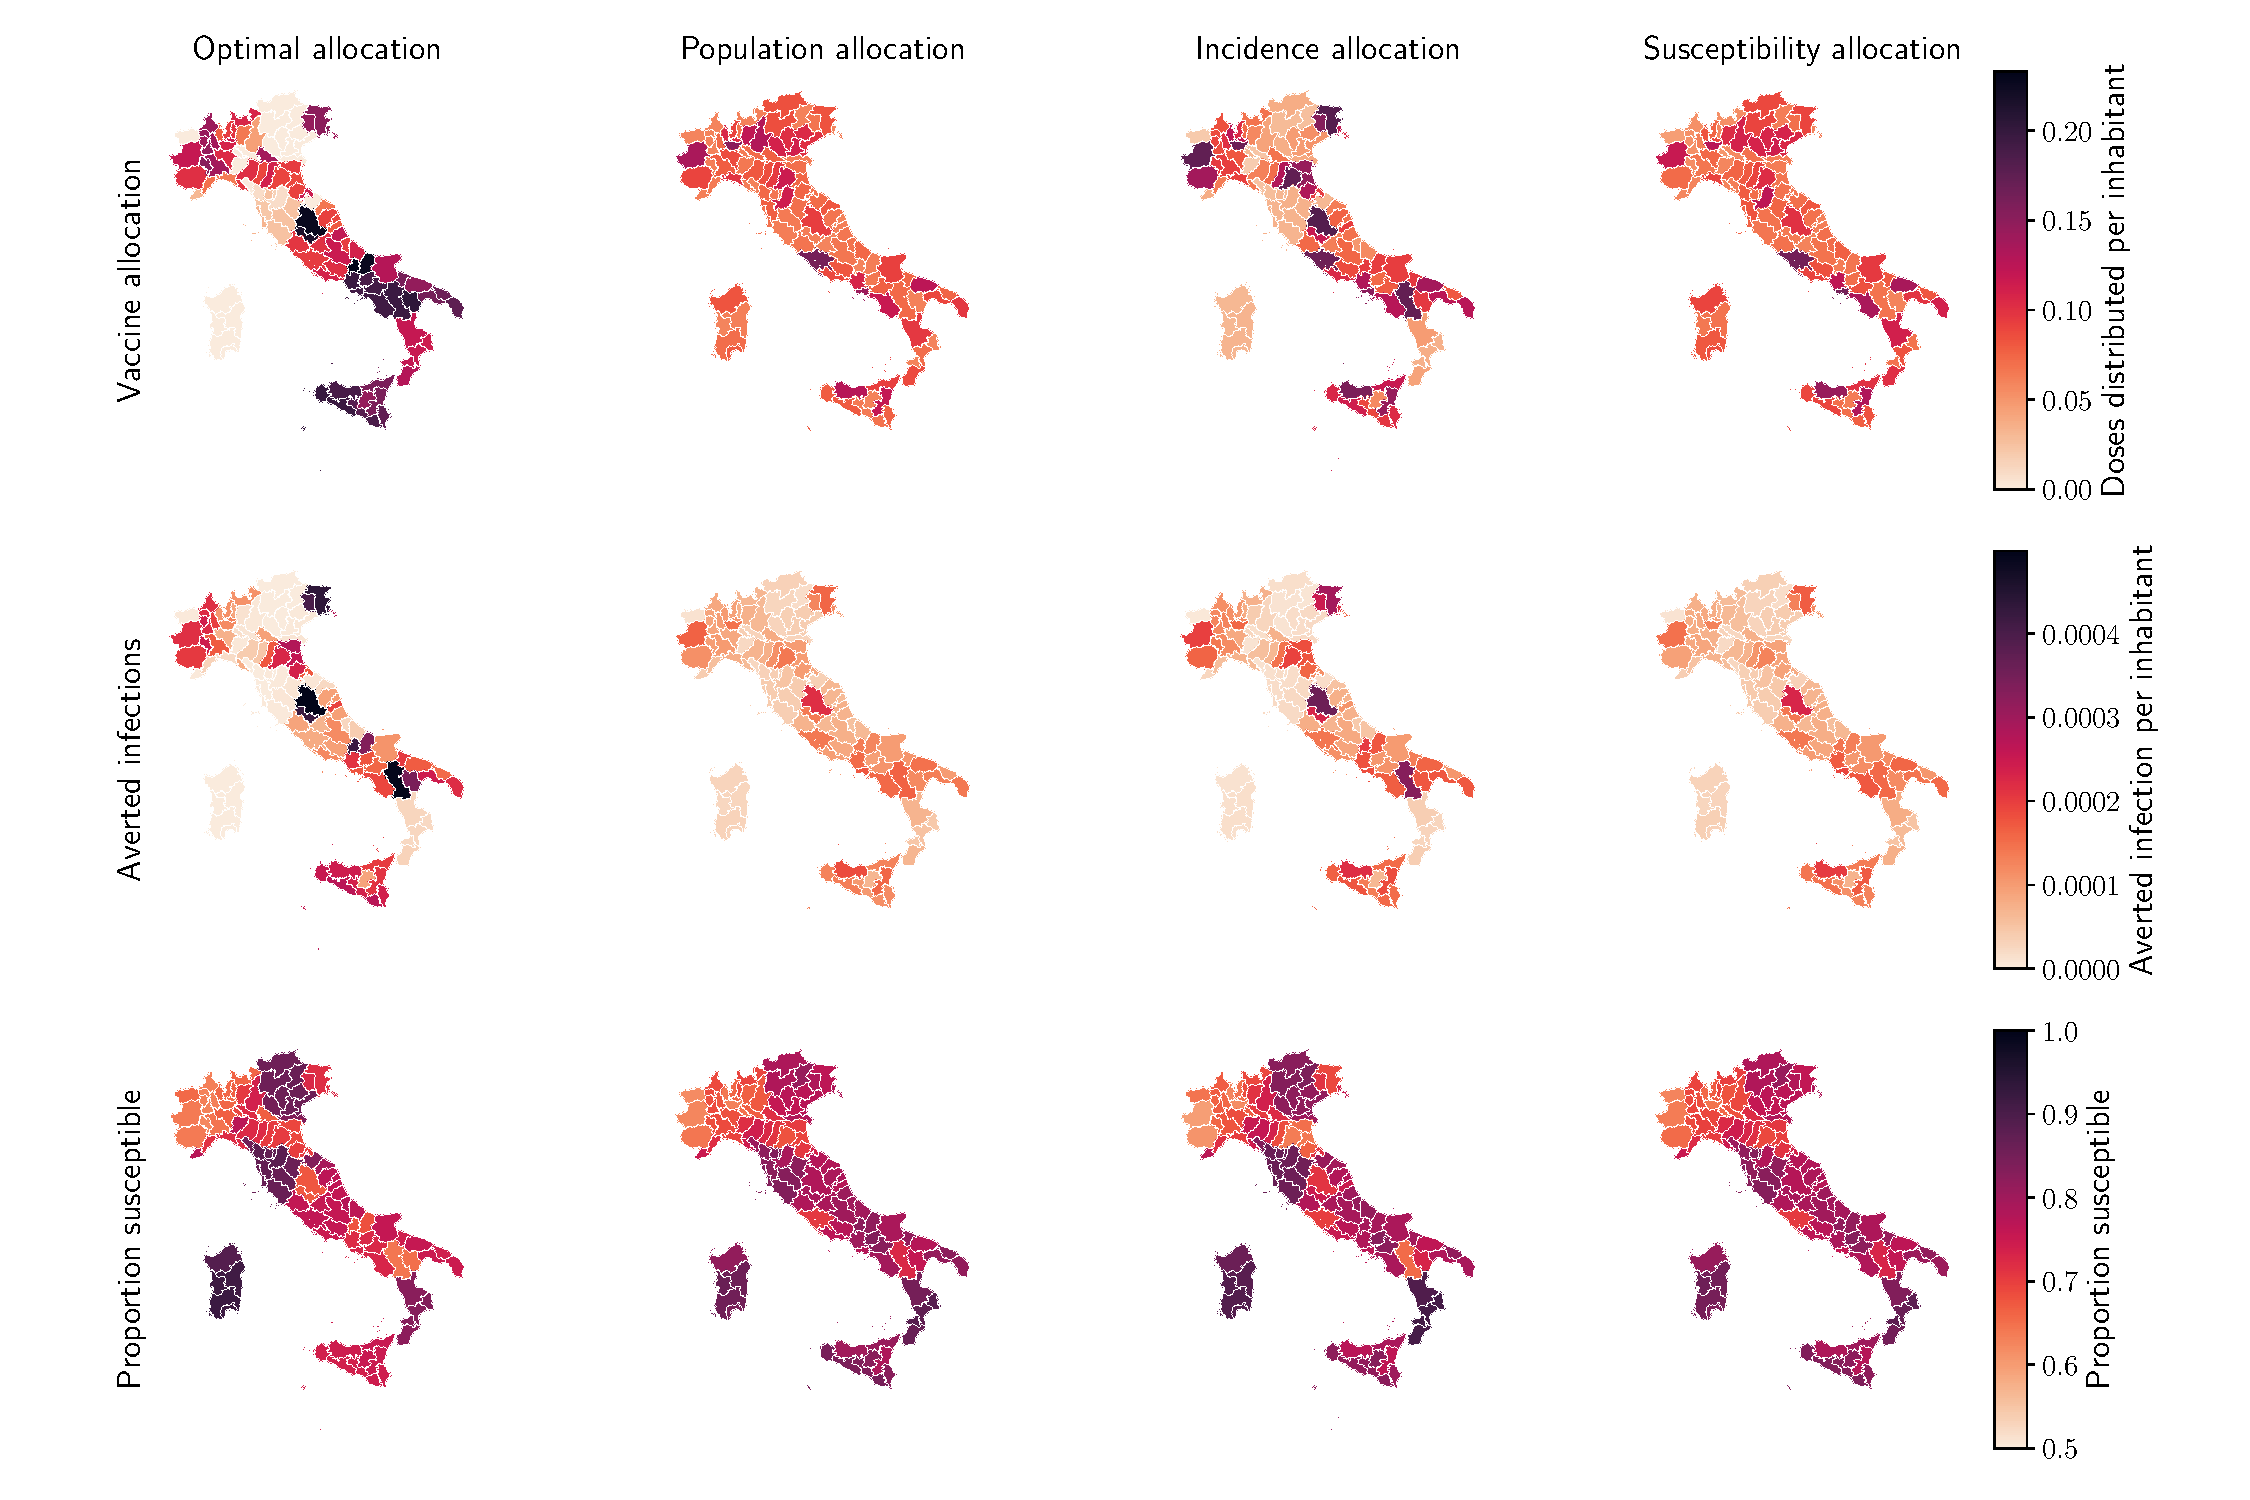
\includegraphics[width=1.1\textwidth]{fig_italy-ocp/figures/map_all.pdf}
    \caption[Spatial  vaccine distribution patterns]{\textbf{Spatial  vaccine distribution patterns} for the optimal allocation (left) and alternative strategies based on population, incidence and susceptibility (additional alternative strategies are presented in SI). We show, for each province and strategy, the proportion of vaccinated individuals (top), the number of averted infections per inhabitant with respect to a no vaccination baseline (middle), and the proportion of individuals who are still susceptible at the end of the control horizon (bottom). Visual inspection suffices to reveal that the optimal allocation strategy is more alike the incidence-based allocation, but with vaccine doses spread-out to more provinces.}
    \label{fig:OC_multimap}
\end{figure*}

Furthermore, we observe in the optimal solution that every time a province is vaccinated, the rate of vaccination is equal to the maximum rate allowed by the local logistic constraint. This property is common to the alternative vaccination strategies, hence the difference in performance is due to the spatial allocation patterns.% of the optimal strategies provide the edge over the other strategies. 
In Figure \ref{fig:OC_multimap}, one can already see by visual inspection that the optimal allocation distributes most of the available doses on a few provinces with high incidence. These provinces are neither the most connected nor the most populous in Italy. The optimal strategy makes then use of the information on the network connectivity to fine-tune the allocation, and deploys the vaccination on more provinces than the incidence-based strategy. %These little optimizations add up to the significant improvement seen above.

To further investigate these patterns, in Figure \ref{fig:OC_scatter}.A we display the number of administered doses vs the incidence projected without vaccines (the proxy variables leading to the second-best control performance), both normalized according to the resident population in each province. We observe an allocation pattern whereby provinces with a higher incidence receive more vaccines. However, the allocation is non-linear with respect to the projected incidence, suggesting that to better control the epidemic, the optimal allocation strategy takes into account other factors such as the importance of each province within the mobility network, as well as the proportion of susceptibles. When the weekly stockpile delivery is increased, as shown in Figure \ref{fig:OC_scatter}.B, this pattern shifts to the right while remaining qualitatively consistent. Hence, the optimal allocation strategy is robust with respect to the overall vaccine availability constraint, and the same nodes are prioritized. We provide scatter plots with other covariates in SI (Figures \ref{fig:OC_scatter_optimistic}--\ref{fig:OC_scatter_optimistic}). 

\begin{figure*}[!ht]
\centering
\includegraphics[width=0.8\textwidth]{fig_italy-ocp/figures/scatter_top.pdf}
\includegraphics[width=0.8\textwidth]{fig_italy-ocp/figures/scatter_scn.pdf}
\caption[Analysis of the optimal solution]{Analysis of the optimal solution. \textbf{A.} Vaccinated population according to the optimal strategy against the projected incidence without vaccination, both normalized by provincial population size and considering the scenario with a weekly stockpile delivery of 479'700 doses. \textbf{B.} Same as in A, but considering all four scenarios of weekly stockpile replenishment. Each dot represents a province, with dot size proportional to its population.}
    \label{fig:OC_scatter}
\end{figure*}

%\subsection{Equity constraints}
%We add additional constraint to the problem in order to guarantee that everyday, there is less than a two-fold difference between the most vaccinated and the less vaccinated node. The result is shown as pink dots in Figures \ref{fig:OC_comparison}. This property might be desirable for equitable access of vaccine, and the proposed framework allow to find the best possible vaccine allocation with regards to these constraints.

%% ***********************************************************************************************
\section{Discussion and Conclusion}
%% ***********************************************************************************************
Without any constraint on supply, each country would vaccinate its population as fast as possible according to the available infrastructure. However limitations in vaccine supply and rate of delivery are a reality for every country, hence the available doses should be deployed in space and time following a fair and effective strategy. 

In stockpile-limited settings, like most current vaccination campaigns worldwide, careful allocation may significantly increase the number of averted infections and deaths. The goal is to distribute the vaccines where they have the strongest beneficial impact on the dynamics of the epidemic. However, deriving an algorithm capable of computing spatially optimal allocation strategies in real, heterogeneous settings is far from trivial and our approach is, to the best of our knowledge, the first attempt in this direction. 

We developed an novel optimal control framework that delivers the best vaccination strategy under constraints on supply and logistics. This allows us to compute the allocation strategy that maximizes the number of averted infections during a projection of the COVID-19 epidemic in Italy from January 11, 2021 to April 11, 2021. Our results show that the optimal strategy has a complex structure that mainly reflects the projected incidence of each province, but also takes into account the spatial connectivity provided by the mobility network and the landscape of acquired population immunity. Although the reason why this strategy is optimal is not immediately intuitive, our simulations clearly outline its better overall performances over other, more straightforward strategies. This comparison suggests that the simplicity underlying intuitive vaccination strategies may undermine their effectiveness, and calls for complementing these simple approaches with rigorous and objective mathematical tools, like optimal control, that allow a full account of the complexity of the problem.

With the present work, we show that it is possible to solve optimal control problems for spatially explicit dynamical models of infectious diseases at a national scale, thus overcoming the computational limitations that, up to now, precluded this kind of applications. The proposed framework can account for any compartmental epidemic model, with up to hundreds of connected spatial nodes. Supply and logistic constraints can be adapted to the actual landscape of decisions faced by the stakeholders, such as no/reduced vaccine delivery on weekends, or the need for fairness in vaccine distribution, e.g. by ensuring that each region receives at least a fixed fraction of the available vaccines. This is especially important as in our optimal allocation scenarios, some provinces receive no vaccine at all. Moreover, the optimization can be carried for single-dose vaccines, as done here, or for two-dose vaccines, where one could potentially optimize the time between the first and second dose (and if a second dose should be administered at all), clearly also considering the intervals recommended by the health authorities.

% Limitations
Our method is obviously not devoid of limitations. The main one is that the optimal vaccination strategy strongly depends on the projection of the underlying epidemiological model. These projections are subject to several sources of uncertainty, especially for long term horizons, for example due to model design and calibration\cite{Cramer:EvaluationIndividualEnsemble:2021}, the generation of baseline transmission scenarios, and unforeseen events that may change the course of the epidemic (such as the importation of cases, the emergence of new virus variants, changes in disease awareness or social distancing policies). The optimal vaccination strategy is thus reliable only if the projections given by the underlying model dynamics are sufficiently accurate. A successful approach developed by the automatic control community to tackle that issue, named Model Predictive Control~\cite{Rawlings:ModelPredictiveControl:2017}, consists in compensating the performance losses expected over long horizons by constantly adapting the optimal strategy. In this context, Model Predictive Control might be implemented using the following steps: (a) at the beginning of each week, the state of the system is estimated by using newly acquired epidemiological data; (b) the optimization problem is solved over a fixed prediction horizon using the estimated state as initial condition; (c) the optimal strategy for the first week is applied and, as soon as the next weeks starts, these steps are repeated starting from (a). This method corrects the model inaccuracies by constantly resetting the initial state to the estimated one. Moreover, constraints may be updated to account for unexpected deliveries or new orders. Future work will aim at further evaluating the benefits of implementing this scheme for the design of optimal vaccination strategies.

Moreover, the epidemiological model underlying our control optimization has known validity and limitations\cite{Gatto:SpreadDynamicsCOVID19:2020, Bertuzzo:GeographyCOVID19Spread:2020}. An additional limitation of the model for the specific scopes of this work is that it does not account explicitly for risk-based classes, and thus does not account for the heterogeneities that may result from the demography of the population, as well as from the age-related transmission and clinical characteristics associated with COVID-19. While surely limiting for operational use of the tools, we note that the scope of this paper is to provide a proof-of-concept of the relevance of spatial effects, which have not been addressed so far in the literature. To that end, we are confident that our results support the relevance of the research question posed. Our framework can anyway be extended to optimize across both spatial and risk heterogeneities. 

A counter-factual assumption in this work is that we consider a one-dose vaccine with full and instantaneous efficacy against transmission. At the time of development, the details about COVID-19 vaccines were not released, and this hypothesis allowed us to demonstrate our framework in a simple setting. Our framework can be further extended to account also for the simultaneous deployment of different vaccine types, some of which may require the administration of two doses. This extension too is subject of ongoing research, in particular to extend the modeling tools described here to accommodate the peculiarities of each authorized vaccine candidate while designing effective spatiotemporal deployment strategies.

% Conclusion
In conclusion, in this work we have optimized vaccine allocation at country scale on different scenarios of epidemic transmission and vaccine availability. Using a data assimilation scheme, we updated a spatially explicit compartmental model that had already been successfully used to describe the COVID-19 pandemic in Italy. To this aim, we have discretized, transformed and simplified the model and constructed a pipeline to perform large-scale nonlinear optimization on vaccine allocation, subject to stockpile and logistic constraints. Solving this problem yielded a complex solution that outperforms other strategies by a significant margin and proves robust across posterior realizations of the underlying model. As such, beside inherent limitations, it provides a benchmark against which other, possibly simpler vaccine rollout strategies can be usefully compared.

%% ***********************************************************************************************
%% ***********************************************************************************************
%% ***********************************************************************************************
\section{Supporting information}
\renewcommand{\thefigure}{S\arabic{figure}}
\renewcommand{\theequation}{S\arabic{equation}}
\setcounter{figure}{0}
\setcounter{equation}{0}
%\SItext
%% ***********************************************************************************************
\subsection*{Optimal control problem}
%% ***********************************************************************************************
The proposed framework is constituted of two disease transmission models, one "true" model and a simplified one used for control:
\begin{itemize}
    \item The full model is a COVID-19 model, as designed in\cite{Gatto:SpreadDynamicsCOVID19:2020, Bertuzzo:GeographyCOVID19Spread:2020}. This model is ODE-based, includes full connectivity based on mobility data, and is implemented in MATLAB using the adaptive step ode45 integration scheme. Using data assimilation, we obtain the joint-posterior distribution for all parameters of this model. 
    \item The simplified model used for optimal control is an approximation of the above model, integrated using an explicit Runge-Kutta 4 method with fixed stepsize. We simplified the problem by limiting the connectivity to the largest mobility fluxes (see Figure \ref{fig:model_description} B) and optimizing only one realization of the posterior. This model is implemented in Python with the CasADi library.
\end{itemize}
This division is necessary in order to solve the optimal control problem (OCP) in a reasonable time. To adapt our framework to another model/country, one would need to update the "true" model to a suitable candidate (which could be a stochastic model, a Hidden Markov model, or any other kind) and design a tractable approximation of this new model to be solved by optimal control.

In order to evaluate the effectiveness of our approach, we first compute the optimal vaccination course that minimizes the objective based on the simplified model. Then, we assess this strategy and the alternative ones on the full model, for different posterior realisations. If the simplified model is sufficiently accurate, the performance loss is small and the proposed strategy outperforms simpler strategies, as shown in our simulation results.

It the subsections below, we first detail the full COVID-19 model, then we describe the optimal control framework and the simplifications we have introduced to bring the problem to a tractable form.

\paragraph{COVID-19 model}
%% ***********************************************************************************************
The optimal control framework may be used with any compartmental SARS-CoV-2 transmission model that can be approximated by ordinary differential equations. To demonstrate its usefulness, we use a complex model based on previous work that was aimed to describe the first wave of COVID-19 infections in Italy\cite{Gatto:SpreadDynamicsCOVID19:2020,Bertuzzo:GeographyCOVID19Spread:2020}. We consider the 107 Italian provinces and the spatial connections induced by human mobility fluxes. In each province, the human population is subdivided according to infection status into the epidemiological compartments of susceptible $S$, exposed $E$, pre-symptomatic $P$ (incubating infectious), symptomatic infectious $I$, asymptomatic infectious $A$, quarantined $Q$, hospitalized $H$, recovered $R$, dead $D$, and vaccinated $V$. The possible transitions between these compartments are shown in Figure \ref{fig:model_description}.A. Individuals in compartments $P$, $A$ and $I$ are infectious and contribute differently to the force of infection, driving susceptible $S$ into incubating individuals $E$. 

The COVID-19 transmission dynamics are described by the following set of ordinary differential equations in each node $i$: 

\begin{equation}\label{eq:sepiar}
\begin{split}
    \dot{S}_i &= - \lambda_i(t) S_i - r^v_i(t) S_i \\
    \dot{E}_i &= \lambda_i(t) S_i -  (\delta^E + r^v_i(t)) E_i \\
    \dot{P}_i &= \delta^E E_i -  (\delta^P+r^v_i(t))  P_i \\
    \dot{I}_i &= \sigma \delta^P P_i - (\gamma^I + \eta)  I_i \\
    \dot{A}_i &= (1 - \sigma) \delta^P P_i - (\gamma^A+ r^v_i(t)) A_i \\
    \dot{Q}_i &= \zeta \eta I_i - \gamma^Q Q \\
    \dot{H}_i &= (1-\zeta) \eta I_i - (\gamma^H + \alpha^H)H \\
    \dot{R}_i &= \gamma^I I_i + \gamma^A A_i + \gamma^H H_i + \gamma^Q Q_i - r^v_i(t) R_i\\
    \dot{V}_i &= r^v_i(t) \cdot (S_i + E_i + P_i + A_i + R_i).
\end{split}
\end{equation}

We define $N_i$ the population of province $i$. Susceptible individuals get exposed to the pathogen at rate~$\lambda_i(t)$, corresponding to the force of infection for community~$i$, thus becoming latently infected (but not infectious yet). Exposed individuals transition to the post-latent, infectious stage at rate~$\delta^E$. Post-latent individuals progress to the next infectious classes at rate $\delta^P$, developing an infection that can be either symptomatic---with probability~$\sigma$---or asymptomatic---with probability $1 - \sigma$. Symptomatic infectious individuals recover from infection at rate~$\gamma^I$ and may seek treatment at rate~$\eta$. Asymptomatic individuals recover at rate~$\gamma^A$.  Infected individuals who sought treatment are either hospitalized (rate $1-\zeta$) or quarantined (rate $\zeta$) at home and are considered to be effectively removed from the community, thus not contributing to disease transmission. Individuals who recover from the infection are assumed to have long-lasting immunity to reinfection at the timescale studied, but possible loss of immunity can be easily included in the model. Hospitalized individuals die at rate $\alpha_H$ and recover at rate $\gamma^H$.

Individuals in compartments $S, E, P, A, R$ might receive vaccine doses. If the chosen strategy allocates $v_{i}(t)$ doses in node $i$ at time t, the vaccination rate is

\begin{equation}
r^v_i(t) = \frac{v_{i}(t)}{S_i(t) +  E_i(t) + P_i(t) + A_i(t) + R_i(t)}
\end{equation}

Vaccinated individuals are moved at rate $r^v_i(t)$ from their original compartments to compartment $V$, where they do not contribute to the infection anymore.

The force of infection of the full model is specified as in Gatto et \textit{al.}\cite{Gatto:SpreadDynamicsCOVID19:2020}, Bertuzzo et \textit{al.}\cite{Bertuzzo:GeographyCOVID19Spread:2020}. In addition to province's local dynamics, it also considers that local susceptibles may enter in contact with infected individuals that are traveling, and oppositely, susceptible commuters may become infected through contact with local infected. The force of infection of the OCP model slightly simplified, and detailed thereafter.

We split the force of infection $\lambda_i(t)$ as the sum of the local force of infection $\lambda^L_i(t)$, from infected in node $i$ and a mobility-driven force of infection from the network $\lambda^N_i(t)$, hence $\lambda_i(t) = \lambda^L_i(t) + \lambda^M_i(t)$. We observe while running our model that $\lambda^M_i(t) \ll \lambda^L_i(t)$. Hence this artificial separation will be exploited when simplifying our model. As described below, we update $\lambda^M_i(t)$ every day whereas $\lambda^L_i(t)$ is updated at each integration step.

As for the formulations of the force of infection, we recall here the formulas designed by\cite{Gatto:SpreadDynamicsCOVID19:2020,Bertuzzo:GeographyCOVID19Spread:2020}. The local force of infection reads:
\begin{equation} 
     \lambda^L_i(t) = C_{i,i} \beta_{0}  \beta_i(t) \cdot \frac{C_{i,i}  (P_i + \epsilon_A  A_i) + \epsilon_I  I_i}{C_{i,i} \cdot (S_i + E_i + P_i + R_i + A_i + V_i) + I_i}, \label{eq:foiL}
\end{equation}
and the influence of other provinces on province $i$ is written as:
\begin{equation}
     \lambda^M_i(t) = \sum_{m, m \neq i} \left( 
     C_{i,m} \cdot 
     \frac{
     \sum_{n, n \neq m} \left[ C_{n,m} \cdot \beta_{0}  \beta_n(t)  (P_n + \epsilon_A  A_n) \right] + \epsilon_I  \beta_{0}  \beta_m(t)  I_m
     }
     {
     \sum_{l, l \neq m}  \left[C_{l, m} \cdot (S_l + E_l + P_l + R_l + A_l + V_l) \right] + I_m
     } 
     \right), \label{eq:foiM}
\end{equation}
where $\beta_{0}$ is the baseline transmission rate, while $\beta_{i}(t)$ is a spatially distributed and time-varying parameter describing site- and time-specific variations in transmissibility due to non-pharmaceutical interventions or other exogenous factors like variants. The parameters $\epsilon_A$ and $\epsilon_I$ represent the reduction of transmission respectively for asymptomatic and symptomatic individuals with respect to pre-symptomatic individual transmissions. Matrix $C$ accounts for mobility: each element $C_{i,j}$ of the matrix ($i \neq j$) represents the proportion of individuals moving from $i$ to $j$, while the diagonal elements $C_{i,i}$ are the proportions of individual who do not move in each node $i$.

The objective for our model is to minimize the total incidence of infections, i.e., $\int_{t_i}^{t_f} \sum_i \lambda_i(t) S_i$. Note that for the present model, this is equivalent to optimizing the total deaths or hospital admissions, as without risk-classes the sizes of these two compartments are proportional to each other.

%% ***********************************************************************************************
\paragraph{Optimal control}
%% ***********************************************************************************************
\begin{figure*}[!ht]
    \centering
    \includegraphics[width=1\textwidth]{fig_italy-ocp/figuresSI/SI_constraint_dist.pdf}
    \caption[Local maximum vaccination rate for each province]{Local maximum vaccination rate $v_i^\mathrm{max}$ for each province. This logistic constraint bounds the maximum number of vaccines to 0.5M of doses per day, with a local rate that is proportional to the node population. Here we show the maximum vaccination rate for each province (the constraint the solution has to comply with), in red, and the maximum rate prescribed by the optimal solution while simulating the pessimistic scenario with a stockpile delivery of 479'700 doses, in black. The optimal solution uses the maximal capacity of the logistic network, while respecting the constraint defined.}
    \label{fig:OC_logistic_constraints}
\end{figure*}

We lump the epidemiological compartments of each node $i$ in variable $x_i(t)=(S_i(t),E_i(t),P_i(t),I_i(t),A_i(t),Q_i(t),H_i(t),R_i(t),V_i(t))$ and we define $v_i(t)$ as our control variable, representing the number of vaccines administered in node $i$ at time $t$. We express the dynamics of the epidemiological model (Equation~\eqref{eq:sepiar}) as an ordinary differential equation in each province $i$:
\begin{equation}
    \label{eq:sepiar_compact}
    \dot x_i(t) = F_i(x_i(t),v_i(t), m_i(t), t),
\end{equation}
where $m_i(t)$ carries the contribution of other provinces to the force of infection of node $i$. For simplicity, we drop the time dependence in the equations below, and we define the state and control variables for the full system as

\begin{align*}
    x = (x_1,\ldots,x_n), && v = (v_1,\ldots,v_n),
\end{align*}

where $n$ is the number of spatial node considered ($n=107$). The global dynamics for all provinces are denoted:

\begin{equation*}
    F(x,v) = (F_1(x_1,v_1, m_1),\ldots,F_n(x_n,v_n, m_n)).
\end{equation*}

The coupled force of infection in node $i$ is denoted $\lambda_i$. We define the cost function as the sum of total incidence of infections (transitions $S_i\longrightarrow E_i$) for every node $i$, i.e.,

\begin{equation*}
    L(x,v) = \sum_{i=1}^n \lambda_i S_i.
\end{equation*}

For the sake of generality, we introduce the terminal cost $M$, which can be used to ensure that we leave the system in a proper state instead of optimizing for short-term gain. Since properly designing the terminal cost could require a long analysis, for simplicity we do not use it in this work, hence $M(\cdot) = 0$.

Given our dynamical system with states $x$, controls $v$, and dynamics $F$, the OCP is:

\begin{subequations}
    \label{eq:ocp}
    \begin{align}
        \min_{v(\cdot)} \ \ & \int_{0}^{T} L(x(t),v(t)) \ \mathrm{d}t + M(x(T)) \\ \label{eq:ocp_dyn1}
        \mathrm{s.t.} \ \ & x(0) = \hat x_0, \\ \label{eq:ocp_dyn2}
        &\dot x(t) = F(x(t),v(t)), && \forall \, t\in[0,T], \\ 
        &H(x(t),v(t)) \leq 0, && \forall \, t\in[0,T],
    \end{align}
\end{subequations}

where we aim at minimizing the cost function over the prediction horizon $T$, while enforcing the modeled SARS-CoV-2 transmission dynamics (Equations \eqref{eq:ocp_dyn1} and \eqref{eq:ocp_dyn2}). Moreover, constraints on vaccine availability and maximum vaccination rate are lumped in function $H$, which reads:

\begin{subequations}
    \begin{align}
        v_i(t) &\geq 0, && i\in\mathbb{I}_1^n, \label{eq:constr_vacc} \\
        \int_{t_\mathrm{d}}^{t_\mathrm{d}+1} v_i(t) \ \mathrm{d}t &\leq v_i^\mathrm{max} \propto N_i, && i\in\mathbb{I}_1^n,\ t_\mathrm{d} \in \mathbb{I}_0^T,  \label{eq:constr_day} \\
        %\int_{0}^{7t_\mathrm{w}} \sum_{i=0}^n v_i(t) \ \mathrm{d}t &\leq D_{t_\mathrm{w}}, && t_\mathrm{w} \in \mathbb{I}_1^{T/7+1}, \label{eq:constr_week}
        \int_{0}^{t} \sum_{i=1}^n v_i(t) \ \mathrm{d}t &\leq D(t), && \forall \, t\in[0,T], \label{eq:constr_week}
    \end{align}
\end{subequations}

where time is measured in days, and $\mathbb{I}_a^b$ is the set of all integers $a\leq k\leq b$. Equation \eqref{eq:constr_vacc} enforces that one can only distribute a non-negative amount of vaccine doses. Equation \eqref{eq:constr_day} states the logistic constraints, which limit the amount of individuals that can be vaccinated each day in each node to $v_i^\mathrm{max}$; here $t_\mathrm{d}$ is the time at which each day starts. We assume that the daily capacity of each province is proportional to the population size of each node $N_i$, because we assume a fair distribution of the sanitary infrastructure among provinces with regard to population, as shown in SI Figure \ref{fig:OC_logistic_constraints}. The stockpile is materialized by Equation
\eqref{eq:constr_week}, which ensures that the total vaccine allocation across every node does not exceed the total availability $D(t)$. The stockpile is replenished every Monday by the delivery of new vaccines, hence $D(t)$ is a staircase function.

%Taking from where we stopped in Materials and Methods, 
We convert our problem formulation \eqref{eq:ocp} to a nonlinear programming problem using direct multiple shooting. Standard multiple shooting splits the time horizon $[0,T]$ using a time grid $t_0,\ldots,t_N$, with $N+1$ points and $t_0=0$, $t_N=T$. 
The control function is parameterized using basis functions with local support. Common choices are a uniform time grid, i.e., $t_{k+1}=t_k+\delta_t$ and a piecewise constant control function, i.e., $v(t)=v_k$, $t\in [t_k,t_{k+1}]$. The system dynamics are then discretized to obtain a discrete-time system

\begin{align*}
    x_{k+1} = f(x_k,v_k),
\end{align*}

satisfying $x_k=x(t_k)$ for all $k=0,\ldots,N$. Moreover, the cost function is also discretized, to obtain

\begin{align*}
    l(x_k,v_k)=\int_{t_k}^{t_k+1} L(x(t),v(t)).
\end{align*}

We perform the discretization using numerical integration techniques (such as a fourth-order Runge-Kutta scheme, with 50 steps per days) to obtain a good approximation of the true trajectory and cost. Finally, the path constraints $H$ are relaxed and imposed at a finite amount of time instants, here coinciding with the time grid $t_0,\ldots,t_N$. We ought to observe that, since in our case the constraints only involve the controls, we are not introducing any approximation by enforcing these constraints only on this uniform grid. The OCP~\eqref{eq:ocp} is then approximated by the nonlinear programming problem

\begin{subequations}
    \begin{align}
        \min_{x,v} \ \ & M(x_N)+\sum_{k=0}^{N-1} l(x_k,v_k)  \\ 
        \mathrm{s.t.} \ \ & x_0 = \hat x_0 \\
        & x_{k+1} = f(x_k,v_k), && k\in \mathbb{I}_0^{N-1}, \\
        &H(x_k,v_k), && k\in \mathbb{I}_0^{N-1}.
    \end{align}
        \label{eq:ocp_nlp}
\end{subequations}

In~\eqref{eq:ocp_nlp}, both the states $x=(x_0,\ldots,x_N)$ and the controls $v=(v_0,\ldots,v_{N-1})$ are defined as optimization variables, which is a distinguishing trait of multiple shooting as opposed to single shooting. 

The main difficulty in solving~\eqref{eq:ocp_nlp} in the context of this paper is the large dimension of the system and the nonlinearity of the model, which can pose severe issues to the numerical solvers. In the following, we will thus introduce a few simplifications, and we will verify through numerical simulations that these simplifications do not imply large errors in the solution of the OCP. 

We discretize the OCP using a uniform grid with sampling time $\delta t=1\ \mathrm{day}$. We assume that (a) vaccinations are administered instantaneously at the beginning of each day, rather than with a constant rate over the whole day; (b) the force of infection associated with mobility is constant over each day; and (c) the weakest mobility links can be pruned. Thus, each node dynamics can be made independent of the other nodes dynamics by introducing an auxiliary control variable $z$ that is constrained to match the force of infection due to the other nodes at the beginning of each time interval. Then, the dynamics of the decoupled system in each node can be written as:

\begin{align*}
    \dot x_i(t) &= F_i(x_i(t),z_{i,k}), && t\in[t_k,t_{k+1}] \\
    x_i(t_k) &= x_{i,k} + g_i(v_{i,k}), && z_{i,k} = e_i(x).
\end{align*}


\paragraph{Discussion on Simplification (a).}
We ought to remark that, realistically, vaccinations will occur at least eight hours per day. Our assumption, while justified as a computationally convenient approximation of reality, is not a priori worse than assuming that vaccine administration takes place over the whole day. More refined approximations, while in principle possible, pose severe issues because of the nature of the system dynamics. While for most initial values the system dynamics can be easily simulated with time-continuous vaccinations, the system becomes stiff by construction once almost the entire population has been vaccinated. In this case, numerical integration errors can drive the size of some compartments to be negative, which violates the model assumptions and makes the result of the numerical integration meaningless. The main issue in this case is that the optimizer will exploit these inaccuracies in order to reduce the cost. Therefore, this issue is much more evident when solving optimal control problems than when simply simulating the system dynamics. We have investigated some simple approaches to tackle this issue, but no technique yielded satisfactory performances. It is our impression that ad-hoc integration strategies will be required in order to reliably simulate and optimize dynamics with continuous vaccination rates. While this will be the subject of future research, the results obtained with the current approximation have yielded sufficient accuracy.

\paragraph{Discussion on Simplification (b).}
This simplification has been proposed in~\cite{Savorgnan:MultipleShootingDistributed:2011} as an approach to solve distributed optimal control problems by means of multiple shooting. In the original version, the coupling variable $z$ is not necessarily piecewise constant, but rather piecewise polynomial. We have observed in simulations that, for this problem, the piecewise constant parametrization yielded sufficient accuracy.

We discretize the dynamics of each node using an explicit Runge-Kutta integrator of order four, with $50$ integration steps per day. Alternative integrators such as explicit Euler, or implicit Runge-Kutta integrators, yielded similar results. Furthermore, in order to verify the accuracy of the integrator and the impact of the introduced simplifications on the solution accuracy, we simulated the system in open-loop, i.e. we applied the optimal control trajectory to the full model starting from the initial condition provided by the data assimilation scheme.

\paragraph{Discussion on Simplification (c).} We sparsify the mobility matrix by pruning element below a threshold (see Figure \ref{figSI:mobility_simplification}). This operation reduces the number of connection between nodes. Also in this case, we verified through numerical simulations that the introduced simplification had a small impact on the prediction and control accuracy.

\begin{figure*}
\centering
\includegraphics[width=\textwidth]{fig_italy-ocp/figuresSI/mobsimplification.png}
\caption[Simplification of the mobility matrix to obtain a sparse and tractable problem]{Simplification of the mobility matrix to obtain a sparse and tractable problem. After the optimization, we assess the effectiveness of the optimal control strategy on the full model.} \label{figSI:mobility_simplification}
\end{figure*}

\paragraph{Possible further improvements} Applying optimal control in open loop, i.e., solving the optimization problem once and applying the control input over the whole time interval, may lead to poor performance due to model inaccuracy and external perturbations. A common remedy consists in closing the loop by repeatedly solving the OCP by using the most updated information on the initial states. This is the principle behind Model Predictive Control (MPC)~\cite{Rawlings:ModelPredictiveControl:2017}. In this context, the state would be estimated on a daily, weekly, or monthly basis so as to solve again the OCP and correct the optimal strategy.

\paragraph{Implementation of the OCP}
We implement the optimal control framework using the automatic differentiation framework CasADi\cite{Andersson:CasADiSymbolicPackage:2012}, the interior-point solver ipopt\cite{Wachter:ImplementationInteriorpointFilter:2006}, and the HSL ma86 large sparse symmetric indefinite solver\cite{HSLCollectionFortran}. The full framework and analysis code is available here: \url{https://github.com/jcblemai/COVID-19_italy-vaccination-oc} (a zenodo DOI will be added after reviews). 

Solving the OCP is both CPU and RAM intensive. For numerical computations, we used the Helvetios cluster the EPFL HPC facility (one problem per computing node, each equipped with 36 2.3 GHz cores and 192 GB RAM). On this cluster, it takes approximately four days to solve the large-scale OCP just presented. It should be possible to solve even larger problems with more RAM available. 

%% ***********************************************************************************************
\subsection*{Data assimilation and model parameters}
%% ***********************************************************************************************
\begin{figure*}
    \centering
    \includegraphics[width=1\textwidth]{fig_italy-ocp/figuresSI/DA_all_sim/hosp.pdf}
    \caption[Modeled daily hospitalizations the against hospitalization data]{Modeled daily hospitalizations (blue) versus hospitalization data (red dots), regional detail of Figure 2.A in the main text. The optimistic and pessimistic transmission scenarios are represented in green and yellow, respectively.}
    \label{fig:SI_DA1}
\end{figure*}
\begin{figure*}
    \centering
    \includegraphics[width=1\textwidth]{fig_italy-ocp/figuresSI/DA_all_sim/incidence.pdf}
    \caption[Modeled daily incidence against the daily reported cases]{Modeled daily incidence (blue) versus the daily reported cases (red dots), regional detail of Figure 2.B in the main text. The optimistic and pessimistic transmission scenarios are represented in green and yellow, respectively.}
    \label{fig:SI_DA2}
\end{figure*}

The regional transmission rates are the main parameters governing the force of infection of the model and, thus, the daily exposed individuals. To better track possible changes in the transmission rates, we adopt a data assimilation strategy based on an iterative particle filter\cite{Manoli:IterativeParticleFilter:2015} used on a moving window of 14 days. The filter starts considering $N_r=1000$ model realizations at time $t_0$ (February 21st, 2020), whose state variables are $x_0^{(j)}, j=1,\dots, N_r$, where the superscript $(j)$ is the realization index and the subscript is the temporal index. Each realization is associated with a parameter combination that is randomly sampled from the posterior distribution evaluated in\cite{Bertuzzo:GeographyCOVID19Spread:2020}, indicated with $\theta^{(j)}$. Possible spatial heterogeneities in regional transmission on a given day $t_k$ are obtained multiplying the transmission parameter by a coefficient $\phi_{k,i}^{(j)}$, where $i$ is the region's index. At time $t_0$, the coefficients $\phi_{0,i}^{(j)}$ are sampled from a truncated normal distribution (mean $\mu_0=1$, standard deviation 0.4, bounds $0.8\mu$-$1.2\mu_0$).
At time $t_k$, we assume to know the state variables $x_k^{(j)}$ and coefficients $\phi_{k,i}^{(j)}$, the latter having ensemble mean $\mu_{k,i}$. To update state variables and coefficients at time $t_{k+1}$, we consider the observations (daily hospitalizations) collected in a temporal window of $\tau=14$ days, $(t_k,t_{k}+\tau$. New coefficients from the truncated normal distribution (mean $\mu_k=1$, standard deviation 0.4, bounds $0.8\mu_k$-$1.2\mu_k$) are sampled at time $\tau=t_0+14$ days.  For each realization, we run the model during the window of 14 days, assuming that the coefficients change linearly for a week, from  $\phi_{0,i}^{(j)}$ to $\tilde{\phi}_{0,i}^{(j)}$, and remain constant afterwards.
The regional likelihood of each realization is then evaluated during these two weeks considering that the daily hospitalizations follow a gamma distribution (as in\cite{Bertuzzo:GeographyCOVID19Spread:2020}). 
A resampling step (systematic resampling , see, e.g.\cite{Douc:ComparisonResamplingSchemes:2005}) selects and duplicates the coefficients $\tilde{\phi}_{0,i}^{(j)}$ associated with the largest likelihood values. These coefficients are then used to update the mean value $\mu_k$. Finally, the simulation is repeated on the same temporal window by sampling new coefficients $\tilde{\phi}_{0,i}^{(j)}$ from the truncated normal distribution with the updated mean $\mu_k$. This set of coefficients is used to compute state variables and parameters at time $t_k$, and then as starting condition to produce the projections used in the main text.

Model parameters (in the absence of vaccination) are taken from a paper\cite{Bertuzzo:GeographyCOVID19Spread:2020} where they were inferred in a Bayesian framework for the period February~24th -- May~1st, 2020, on the basis of the official epidemiological bulletins released daily by Dipartimento della Protezione Civile\cite{DipartimentodellaProtezioneCivile:EmergenzaCoronavirusRisposta} (data available online at {\url{https://github.com/pcm-dpc/COVID-19}}) and the bulletins of Epicentro, at Istituto Superiore di Sanit{à}\cite{IstitutoSuperiorediSanita:CoronavirusUltimiAggiornamenti:2020,Palmieri:CharacteristicsCOVID19Patients:2020}. All the parameters estimated for the initial phase of the Italian COVID-19 epidemic, including the transmission rates, are spatially homogeneous\cite{Bertuzzo:GeographyCOVID19Spread:2020}. This parameterization has been used to produce all the results presented in the main text.


%% ***********************************************************************************************
\paragraph{Spatial set-up} 
%% ***********************************************************************************************
The modeling tools described in the following sections are applied to the Italian COVID-19 epidemic at the scale of second-level administrative divisions, i.e. provinces and metropolitan cities (currently, as of 2021, $107$ spatial units). Official data about resident population at the provincial level is produced yearly by the Italian National Institute of Statistics (Istituto Nazionale di Statistica, ISTAT; data available at\\ \url{http://dati.istat.it/Index.aspx?QueryId=18460}). The latest update (January 1, 2019) has been used to inform the spatial distribution of the population. %For the age-stratified model the data also comes from ISTAT, in the 2018 census: \url{http://demo.istat.it/popres/index.php?anno=2018&lingua=eng}.

The data to quantify nation-wide human mobility come from ISTAT (specifically, from the 2011 national census; data available online at \url{https://www.istat.it/it/archivio/139381}). Mobility fluxes, mostly reflecting commuting patterns related to work and study purposes, are provided at the scale of third-level administrative units (municipalities)\cite{Pepe:COVID19OutbreakResponse:2020,Vollmer:Report20Using:2020}. These fluxes were upscaled to the provincial level following the administrative divisions of 2019, and used to evaluate the fraction $p_i$ of mobile people in each node~$i$, as well as the fraction $q_{ij}$ of mobile people who move between~$i$ and all other administrative units~$j$ (see Supplementary Material in\cite{Gatto:SpreadDynamicsCOVID19:2020}).

%% ***********************************************************************************************
\subsection*{Alternative strategies}
%% ***********************************************************************************************
We designed alternative strategies to compare the optimal solutions. Each strategy uses a decision variable, $\mathcal{V}_i$, as a basis for the allocation of vaccines among provinces. The decision variable is one of:
\begin{itemize}
    \item \textbf{modelled future incidence, absolute}: the modelled total future incidence in a no-vaccination scenario. This is equivalent to the objective of the optimal control problem with no control;
    \item \textbf{modelled future incidence, per population}: as above, but normalized by the resident population in each node;
    \item \textbf{modelled initial susceptibility, absolute}: the modelled number of susceptibles in each province at the start of the vaccination campaign;
    \item \textbf{modelled initial susceptibility, per population}: as above, but normalized by the resident population in each node;
    \item \textbf{province's population}.
\end{itemize}

We define two strategies to distribute the doses:
\begin{itemize}
\item \textbf{Focused} Where every province is sorted (higher on top) according to its decision variable $\mathcal{V}_i$. We then allocate the maximum local rate $v_i^{max}$ to every province going down through the list, until the stockpile is empty. In other words, assuming we have an amount $K$ of vaccines in the stockpile, we find the province index $i$ that satisfy $\max_i \mathcal{V}_i$, and we assign to province $i$ $M_i = \min(v_i^{max}, K)$ vaccines. Then, we find the province $j$ that satisfy $\max_{j,j\neq i} \mathcal{V}_j$ and we assign it $M_j = \min(v_j^{max}, K-M_i)$. And so on, until no vaccine remains in the stockpile. This strategy will concentrate the allocation on nodes with the highest values of the considered decision variable.
\item \textbf{Proportional} In this case, assuming that on a given day there is a quantity of vaccine $K$ in the stockpile, we assign to each province $i$ an amount $M_i = \min(v_i^{max}, K \cdot \frac{\mathcal{V}_i}{\sum_j \mathcal{V}_j})$. This approach vaccinate each node proportionally to the value of its decision variable $\mathcal{V}_i$.
\end{itemize}
In the main text, we show the results for three alternative strategies, namely \textit{proportional absolute incidence}, \textit{proportional population}, and \textit{proportional susceptibility}---named respectively Incidence, Population, and Susceptibility. These strategy are good performers across scenarios, and show how different choices for the decision variables may affect the outcomes of the OCP. In the next sections, we will show the results for all these alternative strategies.

%% ***********************************************************************************************
\subsection*{Additional results for the spatial model}
%% ***********************************************************************************************
We present the results for all these strategies in Table \ref{table:all_strat}, and we show them side-by-side in Figure \ref{fig:OC_comparison_all}. The optimal solutions outperforms all the others solution. In fact, for every given posterior realisation, the optimal control solution always outperforms all other allocation strategies. Even if we observe some scatter when sampling the posterior, the performances of optimal strategies are clearly separated from the rest of the alternatives.

To further investigate the features of the optimal solution, we present a linear scatter plot of the optimal proportion of vaccinated individuals per province (sorting variable) side by side with the province population, the projected incidence without vaccination, and the proportion of susceptible individuals at the start of the simulation. We present these results for the optimistic scenario in Figure \ref{fig:OC_scatter_optimistic} and for the pessimistic scenario in Figure \ref{fig:OC_scatter_pessimistic}. We find no clear visual pattern associating these covariates to the optimal proportion vaccinated, highlighting again that the optimal allocation uses the epidemiological variable in a non-straightforward way, different from every simple strategy we could come up with.

Finally, to highlight the temporal dimension of the prioritization strategy for the deployment of vaccine doses, we present an example of epidemiological dynamics in every compartment of the model for an optimal scenario (Figure \ref{fig:OC_ts_all}), and a stackplot of the proportion of vaccine dose allocated in each province according to the optimal solution (Figure \ref{fig:OC_temporal_alloaction}).

\begin{table*}[h!]
\centering
\tiny
\begin{tabular}{llrrrr}
\toprule
& {} & \multicolumn{2}{c}{Averted Infections} & \multicolumn{2}{c}{Averted Infections} \\
&    &  & & \multicolumn{2}{c}{per dose} \\
Scenario & Method &  Optimistic & Pessimistic &     Optimistic & Pessimistic          \\
\midrule
2M & Optimal &   6.98M &    30.6M &          0.268 &        1.18 \\
        & Incidence &   6.32M &    28.1M &          0.243 &        1.08 \\
        & Proportional Incidence &   6.23M &    27.5M &          0.239 &        1.06 \\
        & Focused Susceptibility &   6.03M &    26.9M &          0.232 &        1.03 \\
        & Focused Proportional Susceptibility &   6.03M &    26.9M &          0.232 &        1.03 \\
        & Focused Proportional Incidence &   6.03M &    26.9M &          0.232 &        1.03 \\
        & Focused Population &   6.03M &    26.9M &          0.232 &        1.03 \\
        & Focused Incidence &   6.03M &    26.9M &          0.232 &        1.03 \\
        & Population &   6.02M &    26.8M &          0.231 &        1.03 \\
        & Susceptibility &   5.97M &    26.7M &          0.229 &        1.02 \\
        & Proportional Susceptibility &    5.6M &    25.3M &          0.215 &       0.971 \\
1.5M & Optimal &   5.52M &    24.1M &          0.283 &        1.24 \\
        & Incidence &   4.89M &    21.7M &           0.25 &        1.11 \\
        & Proportional Incidence &   4.82M &    21.3M &          0.246 &        1.09 \\
        & Focused Population &   4.58M &    20.5M &          0.235 &        1.05 \\
        & Focused Incidence &   4.58M &    20.5M &          0.235 &        1.05 \\
        & Focused Proportional Incidence &   4.58M &    20.5M &          0.235 &        1.05 \\
        & Focused Proportional Susceptibility &   4.58M &    20.5M &          0.235 &        1.05 \\
        & Focused Susceptibility &   4.58M &    20.5M &          0.235 &        1.05 \\
        & Population &   4.57M &    20.4M &          0.234 &        1.05 \\
        & Susceptibility &   4.51M &    20.3M &          0.231 &        1.04 \\
        & Proportional Susceptibility &   4.18M &     19.0M &          0.214 &       0.975 \\
1M & Optimal &    3.9M &    16.9M &            0.3 &         1.3 \\
        & Incidence &   3.41M &    15.1M &          0.262 &        1.16 \\
        & Proportional Incidence &   3.34M &    14.7M &          0.257 &        1.13 \\
        & Focused Population &   3.09M &    13.9M &          0.238 &        1.07 \\
        & Focused Susceptibility &   3.09M &    13.9M &          0.238 &        1.07 \\
        & Focused Proportional Susceptibility &   3.09M &    13.9M &          0.238 &        1.07 \\
        & Focused Incidence &   3.09M &    13.9M &          0.238 &        1.07 \\
        & Focused Proportional Incidence &   3.09M &    13.9M &          0.238 &        1.07 \\
        & Population &   3.08M &    13.8M &          0.237 &        1.06 \\
        & Susceptibility &   3.02M &    13.7M &          0.232 &        1.05 \\
        & Proportional Susceptibility &   2.75M &    12.6M &          0.211 &       0.972 \\
479'700 & Optimal &   1.96M &    8.39M &          0.314 &        1.34 \\
        & Focused Proportional Incidence &   1.95M &    7.74M &          0.312 &        1.24 \\
        & Proportional Incidence &   1.69M &    7.32M &          0.271 &        1.17 \\
        & Incidence &   1.63M &    7.21M &          0.262 &        1.15 \\
        & Focused Incidence &   1.59M &    6.64M &          0.254 &        1.06 \\
        & Focused Population &   1.57M &    6.85M &          0.251 &        1.09 \\
        & Population &   1.45M &    6.57M &          0.233 &        1.05 \\
        & Focused Susceptibility &   1.45M &    6.53M &          0.232 &        1.04 \\
        & Susceptibility &   1.41M &    6.43M &          0.225 &        1.03 \\
        & Focused Proportional Susceptibility &   1.28M &    6.09M &          0.204 &       0.973 \\
        & Proportional Susceptibility &   1.26M &    5.89M &          0.202 &       0.944 \\
\bottomrule
\end{tabular}
\caption{Absolute number of averted infections for each scenario}
\label{table:all_strat}
\end{table*}

\begin{figure*}[!ht]
    \centering
    \includegraphics[width=0.9\textwidth]{fig_italy-ocp/figuresSI/scenarios_perturb_all_SI.pdf}
    \caption[Comparison of different allocation strategies]{Comparison of different allocation strategies. Percentages of averted infections per vaccine dose from January 11, 2021 to April 11, 2021 using different vaccine distribution strategies for the pessimistic (panel A) and the optimistic (panel B) scenario based on: the optimal solution, the spatial distribution of the population, the amount of susceptible individuals at the beginning of the vaccination campaign, and the projected disease incidence in the absence of control. We optimize a median realization of the modeled posterior (diamonds), and assess the performance on the whole posterior (box plots). The results are normalized by the number of averted infections in the optimized solution (see Table \ref{table:all_strat} for absolute values).}
    \label{fig:OC_comparison_all}
\end{figure*}


\begin{figure}[!ht]
    \centering
    \includegraphics[width=\textwidth]{fig_italy-ocp/figuresSI/SI_scatter_Optimistic.pdf}
    \caption[Control and co-variates for the optimistic scenario]{\textbf{Control and co-variates for the optimistic scenario with a stockpile delivery of 479'700 vaccine doses.}}
    \label{fig:OC_scatter_optimistic}
\end{figure}

\begin{figure}[!ht]
    \centering
    \includegraphics[width=\textwidth]{fig_italy-ocp/figuresSI/SI_scatter_Pessimistic.pdf}
    \caption[Control and co-variates for the pessimistic scenario]{\textbf{Control and co-variates for the pessimistic scenario with a stockpile delivery of 479'700 vaccine doses.}}
    \label{fig:OC_scatter_pessimistic}
\end{figure}

\begin{figure}[!ht]
    \centering
    \includegraphics[width=\textwidth]{fig_italy-ocp/figuresSI/SI_all_states.pdf}
    \caption[Example of the dynamics in all compartments]{\textbf{Example of the dynamics in all compartments} for every node in the pessimistic scenario with a stockpile delivery of 479'700 doses. The lower right plot shows the control variable, the number of doses per day in each province.}
    \label{fig:OC_ts_all}
\end{figure}

\begin{figure}[!ht]
    \centering
    \includegraphics[width=\textwidth]{fig_italy-ocp/figuresSI/SI_ts_optimal_stackplot_proportional.pdf}
    \caption[Time allocation for the pessimistic scenario]{\textbf{Time allocation} for the pessimistic scenario with a stockpile delivery of 479'700. We see for each week, how the 479'700 doses are spread accross the provinces, as percent. This view unravel the temporal pattern in the allocation.}
    \label{fig:OC_temporal_alloaction}
\end{figure}



\chapter*{Conclusion and Perspectives}
\addcontentsline{toc}{chapter}{Conclusion and Perspectives}
\markboth{Conclusion and Perspectives}{}
Each of the five chapters of this thesis present an infectious disease model tailored to tackle a public-health policy related question, whether related to infectious disease transmission pathways or to the effects of control policies. Within the four stage framework defined in the \textsc{Introduction} (fig. \ref{fig:modeling}), different facets of infectious disease modeling are exploited to approach the complex phenomenas that are cholera and \textsc{covid}-19 epidemics. Let's go through this conversation of models one more time.

First, as in classical hypothesis testing, a model might be considered as a simplified representation of reality. Among different hypothesis, the aim is to find the ``true'' model underlying the observed dynamics. This perspective is taken in \textsc{Chapter 2}, where the explanatory power of different pathways for rainfall-mediated cholera transmission are compared. Results stress the importance of rainfall as a covariate for cholera transmission while highlighting the complexity of the mechanistic pathways considered. While context-dependent, it is nevertheless interesting to observe how different transmission routes proposed in the litterature fare on intra-seasonal rainfall events in Juba, South Sudan.

In \textsc{Chapters 3} and 4, it is seeked predictive accurary with respect to interventions and transmission of interest; models that most adequately reproduce an unknown, highly complex reality in order to perform experiments are designed\footnote{Indeed, accurate mechanistic modeling is still required for the processes of interest and these two perspectives are more related than opposed}. As a part of multi-modeling study, a spatial stochastic model of cholera transmission in Haiti is proposed in \textsc{Chapter~3}. Building on ECHO's experience on cholera modeling, it is used to assess the probability of cholera elimination from Haiti under different scenarios of mass vaccination campaigns. A restrospective analysis reveals that while the proposed model fits past dynamics, it under-estimates the probability of elimination of cholera in Haiti. This result recalls that modeling is not a silver bullet and stresses the importance of careful model design and that projections uncertainties communication includes modeling assumptions in addition to modeled uncertainty.

Nonwithstanding the \textsc{covid}-19 pandemic, cholera would have been the sole focus of the present thesis. This interuption leave rhe next question unanswered  that derives from these results. There are no confirmed cholera cases since early 2019 in Haiti, which is surprising with regard to the presented modeling work. What is the cause of the extinction of cholera from Haiti ? To what extent did climate, herd immunity and the WaSH interventions carried out in the past year played a role ? Hopefuly the answer will provide additional insights on the path towards elimination of the cholera by 2030, as sought after by WHO and GTFCC. Another open-problem is an open allocation of the cholera vaccine stockpile where demand by countries, and at risk population, vastly exceed supply and production\cite{Pezzoli:GlobalOralCholera:2019}. 

Most of the work undertaken for the response to \textsc{covid}-19 pandemic took place within or around the COVID Scenario Pipeline, a configurable framework to projects epidemic trajectories and healthcare impacts under different suites of interventions. The pipeline is used to support several partners including the state of California and the national US response with report to inform and guide decisions. It is still being actively developed to address the ever-changing need of decision-makers. Since the description given in \textsc{Chapter~4}, a year of historical data brought the need for high-dimensional inference algorithms, and the challenges posed by SARS-CoV-2 have brough it the need for flexible disease transmission and health outcome modeling to capture the dynamics cause by competing strains, immune escape and the different vaccination campaigns. The pipeline is an operational forecasting platform, a goal of the initial research plan, providing a unified framework to project and forecast dynamics from disease emergence to endemicity\footnote{Updated outputs of the pipeline are visible on the \textsc{covid}-19 Scenario Modeling Hub and the \textsc{covid}-19 Forecast Hub (\url{covid19scenariomodelinghub.org} and \url{covid19forecasthub.org}).}.

The assessement of past policies effectiveness is important to project dynamics and to inform decisions. In Switzerland, the pipeline has been used to inform CHUV, Canton de Vaud main hospital. The dialogue with policy makers trigered the exchange of a dataset of lenght of stays in hospital to improve scenario planning report accuracy. In turn, this data has enabled a research study on the estimation of SARS-CoV-2 reproduction number, $R_0$, in Switzerland. Using stochastic models and iterated filtering, a procedure different from most other $R_0$ estimation methods, it uncovers the effectiveness of the non-pharmaceutical interventions in different cantons. Among the numerous takeways from this early \textsc{covid}-19 work presented in \textsc{Chapter 5}, the timing of the decrease in transmission preceeding NPIs implementation is especially interesting. The feedback loop was closed as these estimates were used as assumptions in subsequent modeling reports for Canton de Vaud.


Finally, provided an accurate model of transmission dynamics and interventions effectiveness, an objective and descriptions of operational constraints, optimal control is the ultimate stage of infectious disease modeling towards informed decisions: policies that minimize the burden of a disease are programatically designed. To date both the demanding prerequistes and the difficulty of controling epidemiological models at scales that are useful were hindered the progress on this topic. The optimal control framework is presented in \textsc{Chapter 6} is  Using automatic differenciation and non-linear programing, the proposed solver design the most effective vaccination strategy for a given objective, under operational constraint. A proof of concept is done on vaccination against \textsc{covid}-19 in Italy. While limitations in the model, such as the abscence of age-stratification, limit the scope of the presented results, it is as the first country scale optimization of a comparmental model  a signicant contribution towards making these novel algorithms a tool agaisnt infections disease.

% These models were developed along the same cycle: model \textit{design}$\rightarrow$ model \textit{fit}$\rightarrow$model \textit{adaptation}$\rightarrow$model \textit{insight} to answer scientific and public-health questions. Computer-age statistical inference at the service of infectious disease modeling help to reason about the complex dynamics of epidemics. 


Overall, this thesis is a testament of the relevance of compartmental models as a tools to inform public health decisions, and to reason about infectious disease transmission, providing scientific insights on the underlying processes and the effectiveness of past and future public-health policies. % computer-age

  These two chapters were interesting as after careful model design, results are surprising. More often than not due to an error in the model specification, in this case the investigation enable the discovery of important processes. The studied system is complex and its many interactions and models are an invitation to explore in-depth our belief and assumptions. But sometime model are surprising due to reality being supprising. Or depressing such as the first \textsc{covid}-19 transmission models. 
   In this case careful communication and. Models presented in this thesis have either guided directly decision makers



Yet, the presented research works prove that there is no one-size-fit-all approach to infectious disease modeling, and each research question and transmissions settings requires numerous adjustment to capture and project the dynamics of interests. An unified framework is not possible, and the diversity in approaches is important to tackle.  And even on the same The diversity of sensibilities and background in practitioners bring complementary viewpoint.
  This takeaway might seems discouraging if it is not highlighted that it is not necessary to start from scratch: each model builds on the previous works borrowing conceptuals breakthrough which after some work become tools (taken here in a broad sense encompassing conceptual approaches to software package), developed spefically to be re-used accross settings.
  
%The importance of  These compartmental models share the same backbone and many characteristics, but different features of disease transmission are emphasized to tailor these approach to the research question at stake. 

  Often outbreaks and pandemics have sparked advances on different aspects of infectious disease modeling. The research and public-health communities design new methods and tools leap forward. These advances remains available for endemic diseases and futur pandemic. It improves the preparedness against the emergence of new pathogens, and the response to the \textsc{covid}-19 pandemic has benefitted extensively from conceptual and concrete tools developed from past pandemcis.\footnote{The $R_0$ package and thouroughly used for the \textsc{covid}-19 pandemics was developed after the H1N1 pandemics\fullcite{Obadia:R0PackageToolbox:2012}, comes to mind. Among other topics there are \eg real-time modelisation for Ebola 2014--2015, one-health approach for cholera, multi-modeling studies for influenza, and Zika.}. 
  \marginnote{Apart from \textsc{Chapter 2}, code and data to reproduce these projects are available. However, quality documentation and instructruction are lacking.}
  In addition to the research studies results and conclusions by themselves, it is possible to envision as tools three chapters of the thesis. Arguably, the COVID ScenarioPipeline is already one: it has been used across different settings by different entities. It has proven robust, and recent developement improved its flexibility to allow for other diseases to be modeled. Then in The method to estimate $R_0$, while not novel, is different from most of the current method based either on deconvolutions (backward-forward viewpoint) or parametrized model. While it is involved and necessiate good data and representative assumptions, it works well and provide an alternative look on transmission.
Finally, the optimal control framework allows to explore a model and a disease, from another angle. It is interesting, and slightly dangerous to let the the computer handle the choices to control a complex high-dimenssional  phenomena, just giving it an objective and some constraints. The obtained solution make use of every feature of the model, and one must be careful on the interpretability, these algorithm allow for the design of effective interventions and the best allocation of control ressources. 

As infectious diseases pose a constant threat on children and adults accross the globe, tools and prepardenss to constrction effective interventions are needed. Towards this, improvement in the scientific understandfing of diseases transmissiion, but also the exploration of the facets of the complex system tthat link environement, individuals and societies. While modeling may mislead or render overconfident even in good hands, parcimony and careful inspection makes modeling a key instrument to fight diseases. A point that has been evident during the covid-19 pandemic. In fact, aside from scienfic curiosity lies the neccessity to control infectious disease. Despite tremondous advances, the data about infectious diseases will stay noisy, missing and biased in the foreseable futur. More so because oubreaks thrive where conflicts, natural disaster and instability lies. Mathematical and computational tools to reason about diseases, to infer unknown quantities are a keystone in the path towards elimination, which calls for improvements in every facet of disease control. Tools developed as part of theis thes to better arm in the fight agaisnt futur and exisiting disease. The \textsc{covid}-19 pandemic has exposed what is possible in term of mobilisation and collaboration from partners around the world. The sudden availablity of mobility datasets, something long desired for cholera, is an example of the paradigm shift brought by a pandemic that affected every country in the world. Hopefully, it will set a precedent to involve more partners on great collaborations to tackles other diseases that remains unfair to children and adults worldwide, such as cholera.
And despite limited efficacy, oral cholera vaccines remain a powerful tools, promising in many countries with endemic cholera. 
The course of this thesis has brough reports to decision makers and influenced decisions, and developed tools are a contribution the the arsenal of methods to do se. Towards the elimination of cholera.



\backmatter
%\begin{appendices}\renewcommand{\thefigure}{\textsc{a}\arabic{figure}}
\renewcommand{\theequation}{\textsc{a}\arabic{equation}}
\renewcommand{\thetable}{\textsc{a}\arabic{table}}
\setcounter{figure}{0}
\setcounter{equation}{0}

%\chapter{Appendix to chapter 3}

%\chapter{Appendix to chapter 6}

\chapter{Appendix to chapter 7}

\section{Comment on the simplifications}
\paragraph{Discussion on Simplification (a).}
We ought to remark that, realistically, vaccinations will occur at least eight hours per day. Our assumption, while justified as a computationally convenient approximation of reality, is not a priori worse than assuming that vaccine administration takes place over the whole day. More refined approximations, while in principle possible, pose severe issues because of the nature of the system dynamics. While for most initial values the system dynamics can be easily simulated with time-continuous vaccinations, the system becomes stiff by construction once almost the entire population has been vaccinated. In this case, numerical integration errors can drive the size of some compartments to be negative, which violates the model assumptions and makes the result of the numerical integration meaningless. The main issue in this case is that the optimizer will exploit these inaccuracies in order to reduce the cost. Therefore, this issue is much more evident when solving optimal control problems than when simply simulating the system dynamics. We have investigated some simple approaches to tackle this issue, but no technique yielded satisfactory performances. It is our impression that ad-hoc integration strategies will be required in order to reliably simulate and optimize dynamics with continuous vaccination rates. While this will be the subject of future research, the results obtained with the current approximation have yielded sufficient accuracy.

\paragraph{Discussion on Simplification (b).}
This simplification has been proposed in~\cite{Savorgnan:MultipleShootingDistributed:2011} as an approach to solve distributed optimal control problems by means of multiple shooting. In the original version, the coupling variable $z$ is not necessarily piecewise constant, but rather piecewise polynomial. We have observed in simulations that, for this problem, the piecewise constant parametrization yielded sufficient accuracy.

We discretize the dynamics of each node using an explicit Runge-Kutta integrator of order four, with $50$ integration steps per day. Alternative integrators such as explicit Euler, or implicit Runge-Kutta integrators, yielded similar results. Furthermore, in order to verify the accuracy of the integrator and the impact of the introduced simplifications on the solution accuracy, we simulated the system in open-loop, i.e. we applied the optimal control trajectory to the full model starting from the initial condition provided by the data assimilation scheme.

\paragraph{Discussion on Simplification (c).} We sparsify the mobility matrix by pruning element below a threshold (see Figure \ref{figSI:mobility_simplification}). This operation reduces the number of connection between nodes. Also in this case, we verified through numerical simulations that the introduced simplification had a small impact on the prediction and control accuracy.

\begin{figure*}
\centering
\includegraphics[width=\textwidth]{fig_italy-ocp/figuresSI/mobsimplification.png}
\caption[Simplification of the mobility matrix to obtain a sparse and tractable problem]{Simplification of the mobility matrix to obtain a sparse and tractable problem. After the optimization, we assess the effectiveness of the optimal control strategy on the full model.} \label{figSI:mobility_simplification}
\end{figure*}

\paragraph{Possible further improvements} Applying optimal control in open loop, i.e., solving the optimization problem once and applying the control input over the whole time interval, may lead to poor performance due to model inaccuracy and external perturbations. A common remedy consists in closing the loop by repeatedly solving the OCP by using the most updated information on the initial states. This is the principle behind Model Predictive Control (MPC)~\cite{Rawlings:ModelPredictiveControl:2017}. In this context, the state would be estimated on a daily, weekly, or monthly basis so as to solve again the OCP and correct the optimal strategy.


%% ***********************************************************************************************
%\section{Data assimilation and model parameters}
%% ***********************************************************************************************
%\begin{figure*}
%    \centering
 %   \includegraphics[width=1\textwidth]{fig_italy-ocp/figuresSI/DA_all_sim/hosp.pdf}
  %  \caption[Modeled daily hospitalizations the against hospitalization data]{Modeled daily hospitalizations (blue) versus hospitalization data (red dots), regional detail of Figure 2.A in the main text. The optimistic and pessimistic transmission scenarios are represented in green and yellow, respectively.}
%    \label{fig:SI_DA1}
%\end{figure*}
%\begin{figure*}
%    \centering
%    \includegraphics[width=1\textwidth]{fig_italy-ocp/figuresSI/DA_all_sim/incidence.pdf}
%    \caption[Modeled daily incidence against the daily reported cases]{Modeled daily incidence (blue) versus the daily reported cases (red dots), regional detail of Figure 2.B in the main text. The optimistic and pessimistic transmission scenarios are represented in green and yellow, respectively.}
%    \label{fig:SI_DA2}
%\end{figure*}

%The regional transmission rates are the main parameters governing the force of infection of the model and, thus, the daily exposed individuals. To better track possible changes in the transmission rates, we adopt a data assimilation strategy based on an iterative particle filter\cite{Manoli:IterativeParticleFilter:2015} used on a moving window of 14 days. The filter starts considering $N_r=1000$ model realizations at time $t_0$ (February 21st, 2020), whose state variables are $x_0^{(j)}, j=1,\dots, N_r$, where the superscript $(j)$ is the realization index and the subscript is the temporal index. Each realization is associated with a parameter combination that is randomly sampled from the posterior distribution evaluated in\cite{Bertuzzo:GeographyCOVID19Spread:2020}, indicated with $\theta^{(j)}$. Possible spatial heterogeneities in regional transmission on a given day $t_k$ are obtained multiplying the transmission parameter by a coefficient $\phi_{k,i}^{(j)}$, where $i$ is the region's index. At time $t_0$, the coefficients $\phi_{0,i}^{(j)}$ are sampled from a truncated normal distribution (mean $\mu_0=1$, standard deviation 0.4, bounds $0.8\mu$-$1.2\mu_0$).
%At time $t_k$, we assume to know the state variables $x_k^{(j)}$ and coefficients $\phi_{k,i}^{(j)}$, the latter having ensemble mean $\mu_{k,i}$. To update state variables and coefficients at time $t_{k+1}$, we consider the observations (daily hospitalizations) collected in a temporal window of $\tau=14$ days, $(t_k,t_{k}+\tau$. New coefficients from the truncated normal distribution (mean $\mu_k=1$, standard deviation 0.4, bounds $0.8\mu_k$-$1.2\mu_k$) are sampled at time $\tau=t_0+14$ days.  For each realization, we run the model during the window of 14 days, assuming that the coefficients change linearly for a week, from  $\phi_{0,i}^{(j)}$ to $\tilde{\phi}_{0,i}^{(j)}$, and remain constant afterwards.
%The regional likelihood of each realization is then evaluated during these two weeks considering that the daily hospitalizations follow a gamma distribution (as in\cite{Bertuzzo:GeographyCOVID19Spread:2020}). 
%A resampling step (systematic resampling , see, e.g.\cite{Douc:ComparisonResamplingSchemes:2005}) selects and duplicates the coefficients $\tilde{\phi}_{0,i}^{(j)}$ associated with the largest likelihood values. These coefficients are then used to update the mean value $\mu_k$. Finally, the simulation is repeated on the same temporal window by sampling new coefficients $\tilde{\phi}_{0,i}^{(j)}$ from the truncated normal distribution with the updated mean $\mu_k$. This set of coefficients is used to compute state variables and parameters at time $t_k$, and then as starting condition to produce the projections used in the main text.

%Model parameters (in the absence of vaccination) are taken from a paper\cite{Bertuzzo:GeographyCOVID19Spread:2020} where they were inferred in a Bayesian framework for the period February~24th -- May~1st, 2020, on the basis of the official epidemiological bulletins released daily by Dipartimento della Protezione Civile\cite{DipartimentodellaProtezioneCivile:EmergenzaCoronavirusRisposta} (data available online at {\url{https://github.com/pcm-dpc/COVID-19}}) and the bulletins of Epicentro, at Istituto Superiore di Sanit{à}\cite{IstitutoSuperiorediSanita:CoronavirusUltimiAggiornamenti:2020,Palmieri:CharacteristicsCOVID19Patients:2020}. All the parameters estimated for the initial phase of the Italian COVID-19 epidemic, including the transmission rates, are spatially homogeneous\cite{Bertuzzo:GeographyCOVID19Spread:2020}. This parameterization has been used to produce all the results presented in the main text.


%% ***********************************************************************************************
\paragraph{Spatial set-up} 
%% ***********************************************************************************************
The modeling tools described in the following sections are applied to the Italian COVID-19 epidemic at the scale of second-level administrative divisions, i.e. provinces and metropolitan cities (currently, as of 2021, $107$ spatial units). Official data about resident population at the provincial level is produced yearly by the Italian National Institute of Statistics (Istituto Nazionale di Statistica, ISTAT; data available at\\ \url{http://dati.istat.it/Index.aspx?QueryId=18460}). The latest update (January 1, 2019) has been used to inform the spatial distribution of the population. %For the age-stratified model the data also comes from ISTAT, in the 2018 census: \url{http://demo.istat.it/popres/index.php?anno=2018&lingua=eng}.
The data to quantify nation-wide human mobility come from ISTAT (specifically, from the 2011 national census; data available online at \url{https://www.istat.it/it/archivio/139381}). Mobility fluxes, mostly reflecting commuting patterns related to work and study purposes, are provided at the scale of third-level administrative units (municipalities)\cite{Pepe:COVID19OutbreakResponse:2020,Vollmer:Report20Using:2020}. These fluxes were upscaled to the provincial level following the administrative divisions of 2019, and used to evaluate the fraction $p_i$ of mobile people in each node~$i$, as well as the fraction $q_{ij}$ of mobile people who move between~$i$ and all other administrative units~$j$ (see Supplementary Material in\cite{Gatto:SpreadDynamicsCOVID19:2020}).
The epidemiological data is obtained from the bulletins of the Dipartimento della Protezione Civile, \url{https://github.com/pcm-dpc/COVID-19}).

%% ***********************************************************************************************
\section{Details of the alternative strategies}
%% ***********************************************************************************************
We designed alternative strategies to compare the optimal solutions. Each strategy uses a decision variable, $\mathcal{V}_i$, as a basis for the allocation of vaccines among provinces. The decision variable is one of:
\begin{itemize}
    \item \textsc{modelled future incidence, absolute}: the modelled total future incidence in a no-vaccination scenario. This is equivalent to the objective of the optimal control problem with no control;
    \item \textsc{modelled future incidence, per population}: as above, but normalized by the resident population in each node;
    \item \textsc{modelled initial susceptibility, absolute}: the modelled number of susceptibles in each province at the start of the vaccination campaign;
    \item \textsc{modelled initial susceptibility, per population}: as above, but normalized by the resident population in each node;
    \item \textsc{province's population}.
\end{itemize}

We define two strategies to distribute the doses:
\begin{itemize}
\item \textsc{Focused} Where every province is sorted (higher on top) according to its decision variable $\mathcal{V}_i$. We then allocate the maximum local rate $v_i^{max}$ to every province going down through the list, until the stockpile is empty. In other words, assuming we have an amount $K$ of vaccines in the stockpile, we find the province index $i$ that satisfy $\max_i \mathcal{V}_i$, and we assign to province $i$ $M_i = \min(v_i^{max}, K)$ vaccines. Then, we find the province $j$ that satisfy $\max_{j,j\neq i} \mathcal{V}_j$ and we assign it $M_j = \min(v_j^{max}, K-M_i)$. And so on, until no vaccine remains in the stockpile. This strategy will concentrate the allocation on nodes with the highest values of the considered decision variable.
\item \textsc{Proportional} In this case, assuming that on a given day there is a quantity of vaccine $K$ in the stockpile, we assign to each province $i$ an amount $M_i = \min(v_i^{max}, K \cdot \frac{\mathcal{V}_i}{\sum_j \mathcal{V}_j})$. This approach vaccinate each node proportionally to the value of its decision variable $\mathcal{V}_i$.
\end{itemize}
In the main text, we show the results for three alternative strategies, namely \textit{proportional absolute incidence}, \textit{proportional population}, and \textit{proportional susceptibility}---named respectively Incidence, Population, and Susceptibility. These strategy are good performers across scenarios, and show how different choices for the decision variables may affect the outcomes of the OCP. In the next sections, we will show the results for all these alternative strategies.

%% ***********************************************************************************************
\section{Additional results}
%% ***********************************************************************************************
We present the results for all these strategies in Table \ref{table:all_strat}, and we show them side-by-side in Figure \ref{fig:OC_comparison_all}. The optimal solutions outperforms all the others solution. In fact, for every given posterior realisation, the optimal control solution always outperforms all other allocation strategies. Even if we observe some scatter when sampling the posterior, the performances of optimal strategies are clearly separated from the rest of the alternatives.

To further investigate the features of the optimal solution, we present a linear scatter plot of the optimal proportion of vaccinated individuals per province (sorting variable) side by side with the province population, the projected incidence without vaccination, and the proportion of susceptible individuals at the start of the simulation. We present these results for the optimistic scenario in Figure \ref{fig:OC_scatter_optimistic} and for the pessimistic scenario in Figure \ref{fig:OC_scatter_pessimistic}. We find no clear visual pattern associating these covariates to the optimal proportion vaccinated, highlighting again that the optimal allocation uses the epidemiological variable in a non-straightforward way, different from every simple strategy we could come up with.

\begin{fwtable}
\centering
\small
\begin{tabular}{llrrrr}
\toprule
& {} & \multicolumn{2}{c}{Averted Infections} & \multicolumn{2}{c}{Averted Infections} \\
&    &  & & \multicolumn{2}{c}{per dose} \\
Scenario & Method &  Optimistic & Pessimistic &     Optimistic & Pessimistic          \\
\midrule
2M & Optimal &   6.98M &    30.6M &          0.268 &        1.18 \\
        & Incidence &   6.32M &    28.1M &          0.243 &        1.08 \\
        & Proportional Incidence &   6.23M &    27.5M &          0.239 &        1.06 \\
        & Focused Susceptibility &   6.03M &    26.9M &          0.232 &        1.03 \\
        & Focused Proportional Susceptibility &   6.03M &    26.9M &          0.232 &        1.03 \\
        & Focused Proportional Incidence &   6.03M &    26.9M &          0.232 &        1.03 \\
        & Focused Population &   6.03M &    26.9M &          0.232 &        1.03 \\
        & Focused Incidence &   6.03M &    26.9M &          0.232 &        1.03 \\
        & Population &   6.02M &    26.8M &          0.231 &        1.03 \\
        & Susceptibility &   5.97M &    26.7M &          0.229 &        1.02 \\
        & Proportional Susceptibility &    5.6M &    25.3M &          0.215 &       0.971 \\
1.5M & Optimal &   5.52M &    24.1M &          0.283 &        1.24 \\
        & Incidence &   4.89M &    21.7M &           0.25 &        1.11 \\
        & Proportional Incidence &   4.82M &    21.3M &          0.246 &        1.09 \\
        & Focused Population &   4.58M &    20.5M &          0.235 &        1.05 \\
        & Focused Incidence &   4.58M &    20.5M &          0.235 &        1.05 \\
        & Focused Proportional Incidence &   4.58M &    20.5M &          0.235 &        1.05 \\
        & Focused Proportional Susceptibility &   4.58M &    20.5M &          0.235 &        1.05 \\
        & Focused Susceptibility &   4.58M &    20.5M &          0.235 &        1.05 \\
        & Population &   4.57M &    20.4M &          0.234 &        1.05 \\
        & Susceptibility &   4.51M &    20.3M &          0.231 &        1.04 \\
        & Proportional Susceptibility &   4.18M &     19.0M &          0.214 &       0.975 \\
1M & Optimal &    3.9M &    16.9M &            0.3 &         1.3 \\
        & Incidence &   3.41M &    15.1M &          0.262 &        1.16 \\
        & Proportional Incidence &   3.34M &    14.7M &          0.257 &        1.13 \\
        & Focused Population &   3.09M &    13.9M &          0.238 &        1.07 \\
        & Focused Susceptibility &   3.09M &    13.9M &          0.238 &        1.07 \\
        & Focused Proportional Susceptibility &   3.09M &    13.9M &          0.238 &        1.07 \\
        & Focused Incidence &   3.09M &    13.9M &          0.238 &        1.07 \\
        & Focused Proportional Incidence &   3.09M &    13.9M &          0.238 &        1.07 \\
        & Population &   3.08M &    13.8M &          0.237 &        1.06 \\
        & Susceptibility &   3.02M &    13.7M &          0.232 &        1.05 \\
        & Proportional Susceptibility &   2.75M &    12.6M &          0.211 &       0.972 \\
479'700 & Optimal &   1.96M &    8.39M &          0.314 &        1.34 \\
        & Focused Proportional Incidence &   1.95M &    7.74M &          0.312 &        1.24 \\
        & Proportional Incidence &   1.69M &    7.32M &          0.271 &        1.17 \\
        & Incidence &   1.63M &    7.21M &          0.262 &        1.15 \\
        & Focused Incidence &   1.59M &    6.64M &          0.254 &        1.06 \\
        & Focused Population &   1.57M &    6.85M &          0.251 &        1.09 \\
        & Population &   1.45M &    6.57M &          0.233 &        1.05 \\
        & Focused Susceptibility &   1.45M &    6.53M &          0.232 &        1.04 \\
        & Susceptibility &   1.41M &    6.43M &          0.225 &        1.03 \\
        & Focused Proportional Susceptibility &   1.28M &    6.09M &          0.204 &       0.973 \\
        & Proportional Susceptibility &   1.26M &    5.89M &          0.202 &       0.944 \\
\bottomrule
\end{tabular}
\caption{Absolute number of averted infections for each scenario}
\label{table:all_strat}
\end{fwtable}

\begin{fwfigure}
    \centering
    \includegraphics[width=0.9\textwidth]{fig_italy-ocp/figuresSI/scenarios_perturb_all_SI.pdf}
    \caption[Comparison of different allocation strategies]{Comparison of different allocation strategies. Percentages of averted infections per vaccine dose from January 11, 2021 to April 11, 2021 using different vaccine distribution strategies for the pessimistic (panel A) and the optimistic (panel B) scenario based on: the optimal solution, the spatial distribution of the population, the amount of susceptible individuals at the beginning of the vaccination campaign, and the projected disease incidence in the absence of control. We optimize a median realization of the modeled posterior (diamonds), and assess the performance on the whole posterior (box plots). The results are normalized by the number of averted infections in the optimized solution (see Table \ref{table:all_strat} for absolute values).}
    \label{fig:OC_comparison_all}
\end{fwfigure}


\begin{figure}[!ht]
    \centering
    \includegraphics[width=\textwidth]{fig_italy-ocp/figuresSI/SI_scatter_Optimistic.pdf}
    \caption[Control and co-variates for the optimistic scenario]{Control and co-variates for the optimistic scenario with a stockpile delivery of 479'700 vaccine doses.}
    \label{fig:OC_scatter_optimistic}
\end{figure}

\begin{figure}[!ht]
    \centering
    \includegraphics[width=\textwidth]{fig_italy-ocp/figuresSI/SI_scatter_Pessimistic.pdf}
    \caption[Control and co-variates for the pessimistic scenario]{Control and co-variates for the pessimistic scenario with a stockpile delivery of 479'700 vaccine doses.}
    \label{fig:OC_scatter_pessimistic}
\end{figure}

%\begin{figure}[!ht]
%    \centering
 %   \includegraphics[width=\textwidth]{fig_italy-ocp/figuresSI/SI_all_states.pdf}
  %  \caption[Example of the dynamics in all compartments]{Example of the dynamics in all compartments for every node in the pessimistic scenario with a stockpile delivery of 479'700 doses. The lower right plot shows the control variable, the number of doses per day in each province.}
%    \label{fig:OC_ts_all}
%\end{figure}




\end{appendices}
\begin{fullwidth}\printbibliography\end{fullwidth}

\end{document}